\pdfoutput=1
\documentclass[a4paper,10pt]{amsart}
\title{Cominuscule subvarieties of flag varieties}


\makeatletter
\DeclareRobustCommand{\scotsMc}{\scotsMcx{c}}
\DeclareRobustCommand{\scotsMC}{\scotsMcx{\textsc{c}}}
\DeclareRobustCommand{\scotsMcx}[1]{%
  M%
  \raisebox{\dimexpr\fontcharht\font`M-\height}{%
    \check@mathfonts\fontsize{\sf@size}{0}\selectfont
    \kern.3ex\underline{\kern-.3ex #1\kern-.3ex}\kern.3ex
  }%
}
\expandafter\def\expandafter\@uclclist\expandafter{%
  \@uclclist\scotsMc\scotsMC
}
\makeatother



\author{\texorpdfstring{Benjamin \scotsMc{}Kay}{Benjamin McKay}}

\address{School of Mathematical Sciences,  University College Cork, Cork, Ireland}
\email{b.mckay@ucc.ie}

\thanks{This research was supported in part by the International Centre for Theoretical Sciences (ICTS) during a visit for participating in the program - Analytic and Algebraic Geometry (Code: ICTS/aag2018/03).
This research was largely written at the University of Catania, thanks to the hospitality of the university and of Francesco Russo.
Thanks to Indranil Biswas, Anca \texorpdfstring{Musta\c{t}\u{a}}{Mustata} and Andrei \texorpdfstring{Musta\c{t}\u{a}}{Mustata} for help with algebraic geometry.
This article/publication is based upon work from COST Action CaLISTA, CA21109, supported by COST (European Cooperation in Science and Technology) \url{www.cost.eu}.}
\keywords{flag variety, Hermitian symmetric space}
%\subjclass[2000]{Primary 53B21; Secondary 53C56, 53A55}
\date{\today}

\usepackage{lmodern}
\usepackage{cfr-lm}
\usepackage[T2A,T1]{fontenc}
\usepackage[utf8]{inputenx}
%\usepackage{lineno}
%\linenumbers
\usepackage{siunitx}
\usepackage{xparse}
\usepackage{standalone}
\usepackage{mathtext}
\usepackage[english]{babel}
\usepackage{hyperref}%
\hypersetup{
  colorlinks   = true,  %Colours links instead of ugly boxes
  urlcolor     = black, %Colour for external hyperlinks
  linkcolor    = black, %Colour of internal links
  citecolor    = black  %Colour of citations
}
\usepackage[kerning=true,tracking=true]{microtype}
\usepackage{xspace}
\usepackage{amsfonts}
\usepackage{verbatim}
\usepackage{amssymb}
\usepackage{mathtools}
\usepackage{mathabx}
\usepackage{braket}
\usepackage{cool}
\usepackage{varioref}
\usepackage{xstring}
\usepackage{array}
\usepackage{ragged2e}
\usepackage{longtable}
\usepackage[longtable]{multirow}
\usepackage{booktabs}
\usepackage{enumitem}
\usepackage{varwidth}
\usepackage{tensor}
\usepackage{scalerel}
\usepackage{lie-hasse}
\tikzset{
	background rectangle/.style={
		shade,
		top color=olive!20,
		bottom color=white,
		draw=olive!15,
		very thick,
		rounded corners}}
\usepackage{rank-2-roots}
\usepackage{tikz-cd}
\usepackage{colortbl}
\newtheorem{theorem}{Theorem}
\newtheorem{corollary}{Corollary}
\newtheorem{lemma}{Lemma}
\newtheorem{proposition}{Proposition}
\theoremstyle{remark}
\newtheorem{conjecture}{Conjecture}
\newtheorem{definition}{Definition}
\newtheorem{example}{Example}
\newtheorem{remark}{Remark}
\newtheorem{Comment}{Comment}
\newcounter{remarkCounter}
\setcounter{remarkCounter}{1}
\NewDocumentCommand\todo{m}
{%
    \par\noindent{\textcolor{blue}{\textbf{Comment \#\arabic{remarkCounter}. } #1}}
    \par
    \stepcounter{remarkCounter}
}%
\NewDocumentCommand\finish{}{\todo{Finish this.}}

%% Commands
\NewDocumentCommand\pr{m}{\ensuremath{\left(#1\right)}}
\NewDocumentCommand\curly{m}{\ensuremath{\left\{#1\right\}}}
\NewDocumentCommand\of{m}{\ensuremath{\!\pr{#1}}}
\RenewDocumentCommand\C{o}%
{%
	\ensuremath%
	{%
		\IfValueTF{#1}%
		{%
			\mathbb{C}^{#1}%
		}%
		{%
			\mathbb{C}%
		}%
	}%
}%
\NewDocumentCommand\R{o}%
{%
	\ensuremath%
	{%
		\IfValueTF{#1}%
		{%
			\mathbb{R}^{#1}%
		}%
		{%
			\mathbb{R}%
		}%
	}%
}%
\NewDocumentCommand\Z{o}%
{%
	\ensuremath%
	{%
		\IfValueTF{#1}%
		{%
			\mathbb{Z}^{#1}%
		}%
		{%
			\mathbb{Z}%
		}%
	}%
}%
\NewDocumentCommand\Q{m}%
{%
	\ensuremath%
	{%
		\IfValueTF{#1}%
		{%
			\mathbb{Q}^{#1}%
		}%
		{%
			\mathbb{Q}%
		}%
	}%
}%
\NewDocumentCommand\OPtwo{}{\ensuremath{\mathbb{OP}^2_{\mathbb{C}}}}
\NewDocumentCommand\Proj{m}{\ensuremath{\mathbb{P}^{#1}}}
\NewDocumentCommand\Sym{mm}{\ensuremath{\operatorname{Sym}^{#1}\of{#2}}}
\NewDocumentCommand\GL{m}{\ensuremath{\operatorname{GL}_{#1}}}
\NewDocumentCommand\Lie{mo}{\ensuremath{\mathfrak{\MakeLowercase{#1}}\IfValueT{#2}{_{#2}}}}
\NewDocumentCommand\LieGL{m}{\Lie{GL}[#1]}
\NewDocumentCommand\SL{m}{\ensuremath{\operatorname{SL}_{#1}}}
\NewDocumentCommand\PSL{m}{\ensuremath{\mathbb{P}\!\operatorname{SL}_{#1}}}
\NewDocumentCommand\PSO{m}{\ensuremath{\mathbb{P}\!\operatorname{SO}_{#1}}}
\NewDocumentCommand\PSp{m}{\ensuremath{\mathbb{P}\!\operatorname{Sp}_{#1}}}
\NewDocumentCommand\Gr{smm}%
{%
\ensuremath{\operatorname{Gr}_{#2}\IfBooleanTF{#1}{\of{#3}}{#3}}%
}%
\NewDocumentCommand\SO{m}{\ensuremath{\operatorname{SO}_{#1}}}
\NewDocumentCommand\Symp{m}{\ensuremath{\operatorname{Sp}_{#1}}}
\NewDocumentCommand\normalizer{mm}{\ensuremath{N_{#2}#1}}
\NewDocumentCommand\normalizerAlgebra{mm}{\ensuremath{N_{#2} #1}}
\NewDocumentCommand\centralizer{mm}{\ensuremath{Z_{#2}#1}}
\NewDocumentCommand\centralizerAlgebra{mm}{\ensuremath{Z_{#2} #1}}
\mathtoolsset{centercolon}
\NewDocumentCommand\defeq{}{\coloneqq}
% Define Lie algebra commands \LieX to write out \mathfrak{x}, for X among:
\NewDocumentCommand\MakeLie{m}%
{%
	\expandafter\def\csname Lie#1\endcsname{\Lie{#1}}%
}%
\def\lst{B,G,H,K,L,P,Q,S,Z}
\makeatletter
\@for\i:=\lst\do{\expandafter\MakeLie \i}
\makeatother
\NewDocumentCommand\GN{}{G_+}
\NewDocumentCommand\GZ{}{G_0}
\NewDocumentCommand\breveGZ{}{\breve{G}_0}
\NewDocumentCommand\LieGZ{}{\LieG_0}
\NewDocumentCommand\breveLieGZ{}{\breve{\LieG}_0}
\newcommand*{\Roots}{\Delta}
\newcommand*{\cptRts}{\Delta_0}
\renewcommand*{\aa}{\alpha}
\newcommand*{\bb}{\beta}
\newcommand*{\cc}{\gamma}
\newcommand*{\dd}{\varepsilon}
\newcommand*{\ee}{\sigma}
\newcommand*{\ff}{\tau}

\newcommand*{\XX}[1]{\ensuremath{e_{#1}}}
\NewDocumentCommand\lb{smm}%
{%
\ensuremath{\left[{#2}\IfValueT{#1}{,}{#3}\right]}%
}%
\NewDocumentCommand\free{m}{{#1}^{\textnormal{free}}}

\newcommand{\rtsp}[2]{\ensuremath{{#1}_{#2}}}
\NewDocumentCommand\Pheight{m}{\ensuremath{#1 \cdot e}}
\newcommand*{\ParaRts}{\Delta_{\ge 0}}
\newcommand*{\HH}[1]{\ensuremath{\check #1}}
\newcommand*{\ncptPosRts}{\Delta_+}
\NewDocumentCommand\LieDer{}{\ensuremath{\mathcal L}}


\NewDocumentCommand\drawroots{mm}%
{%
\begin{tikzpicture}[baseline=-.5]
\begin{rootSystem}{#1}
\roots
\parabolic{#2}
\parabolicgrading
\simpleroots
\end{rootSystem}
\end{tikzpicture}
}%
\NewDocumentCommand\mx{m}{{#1}^+}
\NewDocumentCommand\mn{m}{{#1}^-}
\NewDocumentCommand\cp{m}{{#1}^{\degree}}
\makeatletter
\newcommand*{\KillingForm}[2]%
{%%
\ensuremath{%%%
%#1\ifnum\pdf@strcmp{#1}{#2}=\z@ ^2\else\cdot#2\fi
#1\cdot#2
}%%%
}%%
\makeatother
\NewDocumentCommand\KillingSquare{m}%
{%
\ensuremath{#1^2}%
}%
\NewDocumentCommand\om{m}{\omega^{#1}}
\NewDocumentCommand\fl{om}{#2^{\IfValueTF{#1}{#1}{\scriptscriptstyle{\bullet}}}}
\NewDocumentCommand\gr{om}{#2_{\IfValueTF{#1}{#1}{\scriptscriptstyle{\bullet}}}}
% filtered vector space, Lie algebra, module, but remembering only the underlying integer grading.
\NewDocumentCommand\uZ{m}{{}^{\scriptscriptstyle\#}{#1}}
\NewDocumentCommand\odeg{m}{{#1}^{\scriptscriptstyle\#}}
\NewDocumentCommand\agr{som}%
{%
\operatorname{gr}_{\IfValueTF{#2}{#2}{\scriptscriptstyle{\bullet}}}\IfBooleanTF{#1}{(#3)}{\!#3}%
}%


\newcolumntype{C}{>{\columncolor[gray]{.9}}>{$}c<{$}}
\newcolumntype{L}{>{\columncolor[gray]{.9}}>{$}l<{$}}
\newcolumntype{R}{>{\columncolor[gray]{.9}}>{$}r<{$}}
\DeclareMathOperator{\Ad}{Ad}
\DeclareMathOperator{\ad}{ad}

% opposite parabolic subgroup, subalgebra
\NewDocumentCommand\op{m}{#1^{\text{op}}}



\makeatletter
\def\@tocline#1#2#3#4#5#6#7{\relax
  \ifnum #1>\c@tocdepth % then omit
  \else
    \par \addpenalty\@secpenalty\addvspace{#2}%
    \begingroup \hyphenpenalty\@M
    \@ifempty{#4}{%
      \@tempdima\csname r@tocindent\number#1\endcsname\relax
    }{%
      \@tempdima#4\relax
    }%
    \parindent\z@ \leftskip#3\relax \advance\leftskip\@tempdima\relax
    #5\leavevmode\hskip-\@tempdima #6\nobreak\relax
    ,~#7\par
    \endgroup
  \fi}
\makeatother
\arrayrulecolor{white}
\setlength{\arrayrulewidth}{.12em}

\NewDocumentEnvironment{longtabl}{m}%
{%
\renewcommand{\arraystretch}{2}%
\begin{longtable}{#1}%
}%
{%
\end{longtable}%
\renewcommand{\arraystretch}{1}%
}%
\tikzset{
  snake left/.style={
    rounded corners,
    to path={
      let \p1 = (\tikztostart.east),
          \p2 = (\tikztotarget.west),
          \p3 = ($(\p1)!0.5!(\p2)$),
          \n1 = {8pt} 
      in
      (\p1)
      -- (\x1 + \n1, \y1)
      -- (\x1 + \n1, \y3)
      -- (\x2 - \n1, \y3) \tikztonodes
      -- (\x2 - \n1, \y2)
      -- (\p2)
    }
  }
}

\begin{document}
\begin{abstract}
We show that every flag variety contains a natural choice of homogeneous cominuscule subvariety.
From the Dynkin diagram of the flag variety, we compute the Dynkin diagram of that subvariety.
We study the tangent bundles of flag varieties.
\end{abstract}
\maketitle
\begin{center}
\tiny
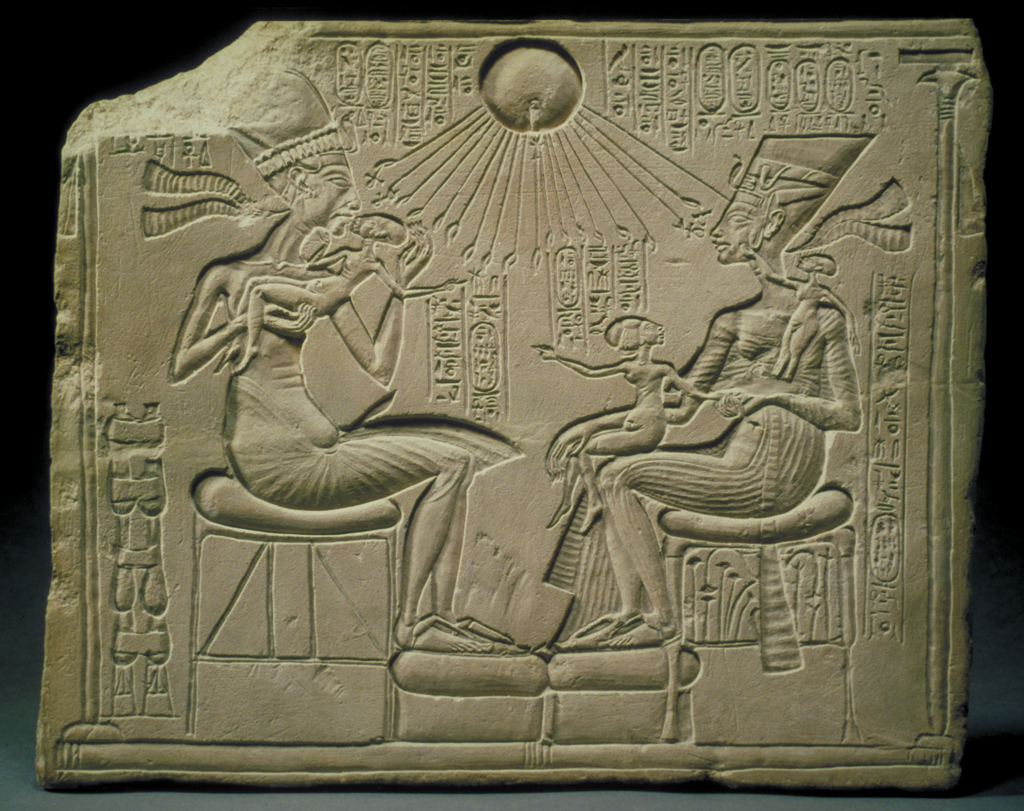
\includegraphics[width=\textwidth]{aten}
Creative Commons Licence, Minneapolis College of Art and Design \\
Attribution 2.0 Generic (CC BY 2.0)
\end{center}
\newpage
\begin{center}
\tableofcontents
\end{center}
\section{Introduction}
We cannot draw a flag variety, or even its associated root system (except in low dimensions), but we can always draw its Hasse diagram.
The Hasse diagrams as drawn by Claus Ringel \cite{Ringel2013} are very clear, so we will follow his conventions.
Our eyes immediately spot in that Hasse diagram its uppermost component, which is always the Hasse diagram of a unique cominuscule variety.
We then predict (correctly, as we will see) that each flag variety contains an associated homogeneous cominuscule subvariety, whose root system is a subsystem of the root system of the flag variety.
Flag varieties have few regular maps between them \cite{bakshi2023morphisms,kumar2023nonexistence,naldi2022morphisms,occhetta2023morphisms,Sierra:2021,Tango:1974,Tango:1976}, hence few flag subvarieties, so these subvarieties are surprising.
Cominuscule varieties are simpler than other flag varieties in many ways; we hope that these cominuscule varieties will shine light on their ambient flag varieties.
We give some evidence for their significance by demonstrating that the associated cominuscule subvariety of any irreducible flag variety is the unique submanifold of maximal symmetry group among all submanifolds satisfying a certain open condition on derivatives.
\begin{example}
As in the image of Aten's rays, pick a point \(p_0\) and a line \(\ell_0\) in the projective plane \(\Proj{2}\), with \(p_0\) not lying on \(\ell_0\).
\[
\begin{tikzpicture}
\clip[rounded corners=10pt] (0,0) -- (4,0) -- (4,2.45) -- (0,2.45) -- cycle;
\node[anchor=south west,inner sep=0] at (0,0) {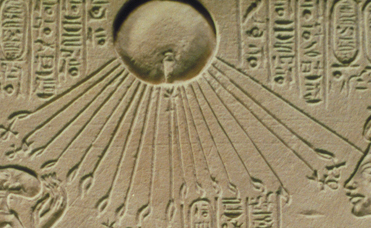
\includegraphics[width=4cm]{aten-crop.jpg}};
\def\x{1.8}
\def\y{2.225}
    \coordinate (sun) at (\x,\y) {};
    \fill[black] (sun) circle (2pt);
%\def\r{.15}
%\def\R{4}
%\begin{scope}
%\clip (0,.75) rectangle (4,2.5);
%   \foreach \i in {7,...,29}
%{
%\draw[rounded corners,white] ({\x+\r*cos(180+5*\i)},{\y+\r*sin(180+5*\i)}) -- ++({\R*cos(180+5*\i)},{\R*sin(180+5*\i)});
%}
%\end{scope}
    \draw[black,ultra thick,rounded corners] (0,.75) -- (4,.75);
\end{tikzpicture}
\]
Each point \(p\) of \(\ell_0\) has an associated pointed line: the pair \((p,pp_0)\).
\[
\begin{tikzpicture}
\clip[rounded corners=10pt] (0,0) -- (4,0) -- (4,2.45) -- (0,2.45) -- cycle;
\node[anchor=south west,inner sep=0] at (0,0) {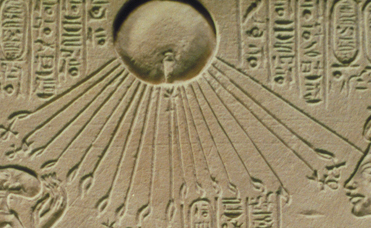
\includegraphics[width=4cm]{aten-crop.jpg}};
\def\x{1.8}
\def\y{2.225}
    \coordinate (sun) at (\x,\y) {};
\def\r{.15}
\def\R{4}
\begin{scope}
\clip (0,.75) rectangle (4,2.5);
\draw[white,thick] (1,.75) -- (\x,\y);
\fill (1,.75) circle (2pt);
%   \foreach \i in {7,...,29}
%{
%\draw[white,opacity=.5,thick] ({\x+\r*cos(180+5*\i)},{\y+\r*sin(180+5*\i)}) -- ++({\R*cos(180+5*\i)},{\R*sin(180+5*\i)});
%}
\end{scope}
    \fill[black] (sun) circle (2pt);
    \draw[black,ultra thick,rounded corners] (0,.75) -- (4,.75);
\end{tikzpicture}
\]
These pointed lines form a rational curve in the variety of pointed lines (\emph{not} in \(\Proj{2}\)). 
\[
\begin{tikzpicture}
\clip[rounded corners=10pt] (0,0) -- (4,0) -- (4,2.45) -- (0,2.45) -- cycle;
\node[anchor=south west,inner sep=0] at (0,0) {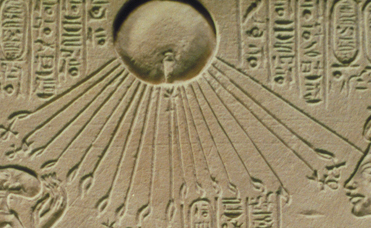
\includegraphics[width=4cm]{aten-crop.jpg}};
\def\x{1.8}
\def\y{2.225}
    \coordinate (sun) at (\x,\y) {};
    \fill[black] (sun) circle (2pt);
\def\r{.15}
\def\R{4}
\begin{scope}
\clip (0,.75) rectangle (4,2.5);
   \foreach \i in {7,...,29}
{
\draw[white,opacity=.5,thick] ({\x+\r*cos(180+5*\i)},{\y+\r*sin(180+5*\i)}) -- ++({\R*cos(180+5*\i)},{\R*sin(180+5*\i)});
}
\end{scope}
    \draw[black,ultra thick,rounded corners] (0,.75) -- (4,.75);
\end{tikzpicture}
\]
This rational curve is homogeneous under the projective transformations fixing \(p_0\) and \(\ell_0\); it is the associated cominuscule variety to the variety of pointed lines.
Each Cartan subgroup of the projective transformations of the plane consists of those projective transformations which preserve three points in general position:
\[
\begin{tikzpicture}
\clip[rounded corners=10pt] (0,0) -- (4,0) -- (4,2.45) -- (0,2.45) -- cycle;
\node[anchor=south west,inner sep=0] at (0,0) {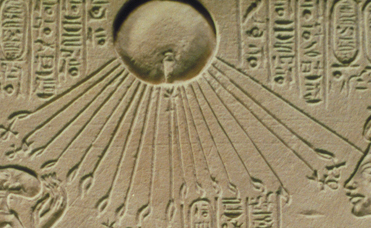
\includegraphics[width=4cm]{aten-crop.jpg}};
\def\x{1.8}
\def\y{2.225}
    \coordinate (sun) at (\x,\y) {};
    \fill[thick,black,draw=white] (sun) circle (2pt);
\def\r{.15}
\def\R{4}
%\begin{scope}
%\clip (0,.75) rectangle (4,2.5);
%   \foreach \i in {7,...,29}
%{
%\draw[rounded corners,white] ({\x+\r*cos(180+5*\i)},{\y+\r*sin(180+5*\i)}) -- ++({\R*cos(180+5*\i)},{\R*sin(180+5*\i)});
%}
%\end{scope}
    \draw[black,ultra thick,rounded corners] (0,.75) -- (4,.75);
    \fill[thick,black,draw=white] (.35,.75) circle (2pt);
    \fill[thick,black,draw=white] (3.5,.75) circle (2pt);
\end{tikzpicture}
\]
Hence the associated cominuscule is invariant under a Cartan subgroup, and conversely there are three associated cominuscules invariant under any given Cartan subgroup.
The projective transformations preserving the point \(p_0\) and line \(\ell_0\) act transitively on the associated cominuscule, moving the points \(p\) of the line \(\ell_0\).
\end{example}
\begin{example}\label{example:flag}
Take a vector space \(V\) and write it as the direct sum of linear subspaces \(V_i\subseteq V\), say of dimension \(n_i\), \(i=1,2,\dots,k\).
Let \(G\defeq\SL{V}\).
Let \(P\subset G\) be the subgroup of linear transformations preserving the successive sums 
\[
V_1,V_1\oplus V_2,\dots,V_1\oplus\dots\oplus V_k=V.
\]
So \(X:=G/P\) is the set of partial flags of dimensions 
\[
0,n_1,n_1+n_2,\dots,n_1+\dots+n_k=n.
\]
Let \(\breve{G}\subset G\) be the subgroup preserving \(V_1\oplus V_k\) and acting as the identity on every \(V_i\), \(i=2,\dots,k-1\).
Let \(\breve{P}\subseteq\breve{G}\) be the subgroup preserving \(V_1\).
Then every element of \(\breve{P}\) preserves \(V_1,V_1\oplus V_2,\dots\), hence \(\breve{P}\subseteq P\).
So \(\breve{X}=\breve{G}/\breve{P}\subseteq X=G/P\) is the Grassmannian inside the partial flag variety \(X\).
The points of \(\breve{X}\) are precisely the partial flags
\[
0=W_0\subset W_1\subset \dots \subset W_k=V
\]
obtained by taking any linear subspace \(W_1\subseteq V_1\oplus V_k\) of the same dimension as \(V_1\), and then taking
\[
W_2:=W_1\oplus V_2, W_3:=W_1\oplus V_2\oplus V_3,\dots,
W_k:=W_1\oplus V_2\oplus\dots\oplus V_k.
\]
In other words,
\[
(V_1\oplus V_k)\cap W_1=W_1, V_2\cap W_1=0,V_3\cap W_1=0,\dots,V_{k-1}\cap W_1=0,
\]
and
\[
V_2\subseteq W_2, V_2\oplus V_3\subseteq W_3, \dots, V_2\oplus\dots\oplus V_{k-1}\subseteq W_{k-1},
\]
i.e.
\[
\dim W_1=\dim((V_1\oplus V_k)\cap W_1),
0=\dim (V_2\cap W_1)=\dots=\dim (V_{k-1}\cap W_1),
\] 
and
\[
\dim (V_2\cap W_2)\ge n_2,\dots,
\dim ((V_2\oplus\dots\oplus V_{k-1})\cap W_{k-1})\ge n_1+\dots+n_{k-1},
\]
so \(\breve{X}\subseteq X\) is an obvious intersection of Schubert cells.
\end{example}
\subsection{Flag varieties}
A \emph{flag variety} \((X,G)\), also called a \emph{generalized flag variety} or a \emph{rational homogeneous variety}, is a complex projective variety \(X\) acted on transitively and holomorphically by a connected complex semisimple Lie group \(G\) \cite{Humphreys:1975} pp.~134--135.
We will need to make use of ineffective flag varieties, i.e. \(G\) might not act faithfully on \(X\).
It is traditional to denote the stabilizer \(G^{x_0}\) of a point \(x_0 \in X\) as \(P\); the subgroup \(P\subseteq G\) is a connected complex linear algebraic subgroup.
A subgroup of \(G\) is \emph{parabolic} if it is the stabilizer of a point of a flag variety \((X,G)\) of \(G\), hence the use of the letter \(P\).

Denote the Lie algebras of \(P\subseteq G\) by \(\LieP\subseteq\LieG\). 
One can select a Cartan subgroup of \(G\) lying inside \(P\), whose positive root spaces all lie in \(\LieP\).
A simple root \(\aa\) is \(P\)-\emph{compact} (\emph{compact} if \(P\) is understood) if the root space of \(-\aa\) belongs to the Lie algebra of \(P\).
Each flag variety is determined uniquely, up to finite central extension of \(G\) and up to isomorphism, by the Dynkin diagram of \(G\) decorated with \(\dynkin{A}{*}\) on each compact simple root and \(\dynkin{A}{x}\) on each noncompact simple root \cite{Borel:1991} p.~197 Proposition 14.18, \cite{Humphreys:1975} p.~197 Theorem${}'$.
\subsection{Reducible flag varieties}\label{subsec:reducible}
The center of any complex semisimple Lie group \(G\) lies in every maximal torus, so in every Cartan subgroup \cite{Borel:1991} p.~220, so in every parabolic subgroup, so acts trivially on every flag variety.
An \emph{irreducible} flag variety is a flag variety \((X,G)\) with \(G\) a simple Lie group, and with only the center of \(G\) acting trivially.
Every flag variety \((X,G)\), up to finite central extension of \(G\), admits a factorization 
\begin{align*}
X&=X_0 \times X_1 \times X_2 \times \dots \times X_s, \\
G&=G_0 \times G_1 \times G_2 \times \dots \times G_s, 
\end{align*}
into irreducible flag varieties \(\pr{X_i, G_i}\), \(i>0\), and a point \(X_0=\set{x_0}\), unique up to permutation of the \((X_i,G_i)\) for \(i>0\) and isomorphism.
The flag variety \((X,G)\) is effective if and only if all \((X_i,G_i)\) are effective, i.e. if and only if \(G_0=\set{1}\) is trivial and \(G_1,\dots,G_s\) are in adjoint form, and then \((X,G)\) is precisely (not just up to finite central extension) \cite{Akhiezer:1995} p.~74 the product 
\begin{align*}
X&=X_1 \times X_2 \times \dots \times X_s, \\
G&=G_1 \times G_2 \times \dots \times G_s.
\end{align*}
\subsection{Cominuscule varieties}
A flag variety is \emph{cominuscule} if \(\LieG/\LieP=T_{x_0} X\) is a sum of irreducible complex algebraic \(P\)-modules.
This occurs just when there is a compact subgroup \(K\subseteq G\) so that \(\pr{X,K}\) is a compact Hermitian symmetric space \cite{Kostant:1961} p.~379 Proposition 8.2, \cite{Baston/Eastwood:1989} p.~26.
Some authors prefer the term \emph{compact Hermitian symmetric space}, \emph{cominuscule Grassmannian}, or \emph{generalized Grassmannian} to \emph{cominuscule variety}.
Every effective cominuscule variety is a product of the following irreducible effective cominuscule varieties \cite{Baston/Eastwood:1989} p.~26, Example~3.1.10, \cite{Kobayashi/Nagano:1964} theorem~1 p.~401:
\newpage
%\par\noindent{}%
%%%\documentclass{amsart}
%\pdfoutput=1
%\usepackage{array}
%\usepackage{longtable}
%\usepackage{xparse}
%\usepackage{colortbl}
%\usepackage{booktabs}
%\usepackage{dynkin-diagrams}
%\NewDocumentCommand\pr{m}{\ensuremath{\left(#1\right)}}
%\NewDocumentCommand\curly{m}{\ensuremath{\left\{#1\right\}}}
%\NewDocumentCommand\of{m}{\ensuremath{\!\pr{#1}}}
%\newcolumntype{C}{>{\columncolor[gray]{.9}}>{$}c<{$}}
%\newcolumntype{L}{>{\columncolor[gray]{.9}}>{$}l<{$}}
%\newcolumntype{R}{>{\columncolor[gray]{.9}}>{$}r<{$}}
%\arrayrulecolor{white}
%\setlength{\arrayrulewidth}{.12em}
%\NewDocumentEnvironment{longtabl}{m}%
%{%
%\renewcommand{\arraystretch}{2}%
%\begin{longtable}{#1}%
%}%
%{%
%\end{longtable}%
%\renewcommand{\arraystretch}{1}%
%}%
%\NewDocumentCommand\C{o}%
%{%
%\IfValueTF{#1}%
%{%
%	\ensuremath{\mathbb{C}^{#1}}%
%}%
%{%
%	\ensuremath{\mathbb{C}}%
%}%
%}%
%\NewDocumentCommand\Proj{m}{\ensuremath{\mathbb{P}^{#1}}}
%\begin{document}
\begingroup
\small
\begin{longtabl}{@{}%
>{\columncolor[gray]{.9}$}r<{$}%
>{\columncolor[gray]{.93}}p{2.6cm}%
>{\columncolor[gray]{.9}$}r<{$}%
>{\columncolor[gray]{.93}}l@{}}
\toprule
G&\(G/P\)&\operatorname{dim}&\text{description}\\
\midrule
\endfirsthead
\toprule
G&\(G/P\)&\operatorname{dim}&\text{description}\\
\midrule
\endhead
\bottomrule
\endfoot
\bottomrule
\endlastfoot
A_r&\dynkin{A}{**.*x*.**}&k(r+1-k)&Grassmannian of $k$-planes in $\C[r+1]$
\\
B_r&\dynkin[parabolic=1]{B}{}&2r-1&quadric hypersurface in $\Proj{2r}$\\
C_r&\dynkin[parabolic=16]{C}{}&\frac{r(r+1)}{2}&space of Lagrangian $r$-planes in $\C[2r]$\\
D_r&\dynkin[parabolic=1]{D}{}&2r-2&quadric hypersurface in $\Proj{2r-1}$\\
D_r&\dynkin[parabolic=32]{D}{}&\frac{r(r-1)}{2}& %one component of the variety of 
space of null $r$-planes in $\C[2r]$ \\
E_6&\dynkin[parabolic=1]{E}{6}&16&complexified octave projective plane\\
E_7 &\dynkin[parabolic=64]{E}{7}&27&space of null octave \(3\)-planes in octave \(6\)-space
\end{longtabl}
\endgroup
%\end{document}
\begingroup
\small
\begin{longtabl}{@{}%
>{\columncolor[gray]{.9}$}r<{$}%
>{\columncolor[gray]{.93}}p{2.6cm}%
>{\columncolor[gray]{.9}$}r<{$}%
>{\columncolor[gray]{.93}}l@{}}
\toprule
G&\(G/P\)&\operatorname{dim}&\text{description}\\
\midrule
\endfirsthead
\toprule
G&\(G/P\)&\operatorname{dim}&\text{description}\\
\midrule
\endhead
\bottomrule
\endfoot
\bottomrule
\endlastfoot
A_r&\dynkin[labels={,,,k,,,}]{A}{**.*x*.**}&k(r+1-k)&Grassmannian of $k$-planes in $\C[r+1]$
\\
B_r&\dynkin[parabolic=1]{B}{}&2r-1&quadric hypersurface in $\Proj{2r}$\\
C_r&\dynkin[parabolic=16]{C}{}&\frac{r(r+1)}{2}&space of Lagrangian $r$-planes in $\C[2r]$\\
D_r&\dynkin[parabolic=1]{D}{}&2r-2&quadric hypersurface in $\Proj{2r-1}$\\
D_r&\dynkin[parabolic=16]{D}{}&\frac{r(r-1)}{2}& %one component of the variety of 
component of space of null $r$-planes in $\C[2r]$ \\
D_r&\dynkin[parabolic=32]{D}{}&\frac{r(r-1)}{2}& %one component of the variety of 
component of space of null $r$-planes in $\C[2r]$ \\
E_6&\dynkin[parabolic=1]{E}{6}&16&complexified octave projective plane\\
E_7 &\dynkin[parabolic=64]{E}{7}&27&space of null octave \(3\)-planes in octave \(6\)-space
\end{longtabl}
\endgroup
%% end input
\subsection{Structure of linear algebraic groups}
A complex linear map is \emph{unipotent} if its only eigenvalue is \(1\).
A subgroup of a linear algebraic group is \emph{unipotent} if it consists of unipotent linear maps.
Every complex linear algebraic group \(G\) has a \emph{unipotent radical}, the unique maximal unipotent normal subgroup, which is a closed complex linear algebraic subgroup \cite{Borel:1991} p.~85 Theorem~4.5, p.~86 Theorem~4.7, p.~157 11.21.

A complex linear algebraic group is \emph{reductive} if it contains a Zariski dense compact subgroup \cite{Vinberg:1994} p.~142 Theorem~2.7, Theorem~2.8.
Every complex linear algebraic group \(G\) has a \emph{reductive Levi factor}, i.e. a maximally reductive complex linear algebraic subgroup,  unique up to conjugacy, so that \(G\) is a semidirect product of its reductive Levi factor and its unipotent radical \cite{Borel:1991} p.~158 11.22.
Any Cartan subgroup is therefore a subgroup of the reductive Levi factor, after perhaps a conjugacy.
Every compact subgroup lies in a maximal compact subgroup, which is unique up to conjugacy, so lies in the reductive Levi factor up to conjugacy \cite{Hilgert.Neeb:2012} p.~531 Theorem~14.1.3.
After perhaps extending by some finite group of order a power of \(2\), the Weyl group embeds in \(G\) as a finite subgroup \cite{Tits:1966}, hence compact, so this group lies in the reductive Levi factor up to conjugacy.

\subsection{Parabolic subgroups}
A Zariski closed subgroup \(P\subseteq G\) of a connected linear algebraic group \(G\) is \emph{parabolic} if \(X:=G/P\) is a projective variety, and this occurs just when \((X,L)\) is a flag variety for a semisimple Levi factor \(L\subseteq G\), and this occurs just when \(P\) contains a Borel subgroup (i.e. a maximal connected solvable subgroup) \cite{Borel:1991} p.~148.
Every parabolic subgroup is connected \cite{Borel:1991} p.~197 Proposition 14.18.
The unipotent radical of \(P\) is denoted \(\GN\subseteq P\), and a reductive Levi factor is denoted \(\GZ\subseteq P\), so \(P=\GZ\ltimes\GN\).
(This is potentially confusing; the reader might expect to write these as \(P_+\) and \(P_0\) since they lie in \(P\), but this notation is standard \cite{Cap/Slovak:2009} p.~293 theorem 3.2.1, and due to the presence of the grading of the Lie algebra of \(G\) which we will define.)
A flag variety is cominuscule just when \(\GN\) is abelian \cite{Cap/Slovak:2009} p.~296 \S{}3.2.3.
Denote the center of the unipotent radical by \(Z\defeq Z_{\GN}\).
\subsection{Opposite parabolic subgroups}\label{subsec:opposite.parabolic}
Two parabolic subgroups \(P,\op{P}\subseteq G\) of a complex semisimple Lie group are \emph{opposite} if \(P\cap\op{P}\) is a reductive Levi factor of both \(P\) and \(\op{P}\).
All Borel subgroups of \(G\) are conjugate \cite{Borel:1991} p.~147 chapter IV 11.1, each containing a Cartan subgroup, hence the Lie algebra of \(P\) is the sum of (1) the Cartan subalgebra with (2) various root spaces.
Every automorphism of a root system arises from an automorphism of the associated semisimple Lie group \cite{Fulton/Harris:1991} p.~498 Proposition D.40, \cite{Humphreys:1978}, p.~87, \S16.5.
Hence there is an automorphism \(G\xrightarrow{a}G\) of \(G\) which yields \(\alpha\mapsto-\alpha\) in the root system.
(We can define such an automorphism explicitly as \(e_{\alpha}\mapsto -e_{-\alpha}\) on root vectors in a Chevalley basis; see \S\vref{subsubsection:ChevalleyBases}.)
Our automorphism sends \(P\) to an opposite parabolic subgroup \(\op{P}:=aP\) with \(P\cap \op{P}=\GZ\).
Letting \(G_-:=aG_+\), \(G_+\cap G_-=\set{1}\).
An open subset of \(G\) consists of elements uniquely expressed as a product \(p,q\in P\times G_-\mapsto pq\in G\) \cite{Cap/Slovak:2009} p.~294, \cite{Borel:1991} p.~198 Proposition 14.21.
Every root system also has an automorphism, traditionally called \(w_0\), which belongs to the Weyl group and which interchanges the positive and negative roots of a root system \cite{Cap/Slovak:2009} pp.~323-324; it is the unique element of the Weyl group of maximum length.
Note that \(w_0\) might not reverse the signs of simple roots \cite{Cap/Slovak:2009} p.~324.
The Weyl group lifts to a group of automorphisms of the Lie group \(G\), after perhaps extension by some finite group of order a power of \(2\).
We can use such an extension of \(w_0\) in place of \(a\) throughout this paper, as we will only need that \(a\) is an automorphism of a given root system which extends to an automorphism of \(G\) taking a given parabolic subgroup to an opposite.
\subsection{Definition of the associated cominuscule}
Take a flag variety \((X,G)\) and opposite parabolic subgroups \(P,\op{P}\subseteq G\), so that \(P\) is the stabilizer of \(x_0\in X\).
As above, take their unipotent radicals \(G_+,\op{G_+}\) and the centers \(Z,\op{Z}\) of these.
Let \(\breve{G}\defeq\left<Z,\op{Z}\right>\subseteq G\) be the subgroup generated by \(Z\cup\op{Z}\), \(\breve{P}\defeq\breve{G}\cap P\), \(\breve{X} \defeq \breve{G}/\breve{P}\).
Then \((\breve{X},\breve{G})\) is the \emph{associated cominuscule subvariety} through the point \(x_0\in X\).
\subsection{Example: the general linear flag variety}
We return to the study of the flag varieties of \(A_{n-1}=\PSL{n}\); see example~\vref{example:flag}.
We took a vector space \(V\) of dimension \(n\).
We let \(G\defeq\PSL{V}\) and \(X\) the set of partial flags of dimensions 
\[
0,n_1,n_1+n_2,\dots,n_1+\dots+n_k=n.
\]
We wrote \(V\) as the direct sum of linear subspaces \(V_i\subseteq V\), say of dimension \(n_i\), \(i=1,2,\dots,k\).
Supposing that \(V=\C[n]\), our automorphism becomes transpose inverse.
To be explicit, for simplicity we suppose \(k=4\).
Let \(G'\subseteq G\) be the subgroup leaving \(\breve{X}\subseteq X\) invariant, and \(P':=G'\cap P\).
In our table, each line is a pair \(\Gamma \ M\), 
of a group \(\Gamma\) and a matrix \(M\) with some unspecified entries, to mean that \(\Gamma\) is the group of unimodular matrices of the given form \(M\), modulo rescaling by the matrices \(\lambda I\) of that form where \(\lambda\) is an \(n^{\textnormal{th}}\) root of unity.
\begin{longtable}{@{}>{$\mathrlap}c<{$}>{$}c<{$}@{}}
G&\begin{pmatrix}
*&*&*&*\\
*&*&*&*\\
*&*&*&*\\
*&*&*&*
\end{pmatrix}\\[3em]
P&\begin{pmatrix}
*&*&*&*\\
0&*&*&*\\
0&0&*&*\\
0&0&0&*
\end{pmatrix}\\[3em]
G_+&
\begin{pmatrix}
I&*&*&*\\
0&I&*&*\\
0&0&I&*\\
0&0&0&I
\end{pmatrix}\\[3em]
Z&\begin{pmatrix}
I&0&0&*\\
0&I&0&0\\
0&0&I&0\\
0&0&0&I
\end{pmatrix}\\[3em]
G_0&\begin{pmatrix}
*&0&0&0\\
0&*&0&0\\
0&0&*&0\\
0&0&0&*
\end{pmatrix}\\[3em]
\breve{G}&
\begin{pmatrix}
*&0&0&*\\
0&I&0&0\\
0&0&I&0\\
*&0&0&*
\end{pmatrix}\\[3em]
\breve{P}&
\begin{pmatrix}
*&0&0&*\\
0&I&0&0\\
0&0&I&0\\
0&0&0&*
\end{pmatrix}\\[3em]
G'&\begin{pmatrix}
*&0&0&*\\
0&*&0&0\\
0&0&*&0\\
*&0&0&*
\end{pmatrix}\\[3em]
P'&
\begin{pmatrix}
*&0&0&*\\
0&*&0&0\\
0&0&*&0\\
0&0&0&*
\end{pmatrix}
\end{longtable}
To be more precise, \(G_+\) consists of the matrices 
\[
\begin{pmatrix}
\lambda I&*&*&*\\
0&\lambda I&*&*\\
0&0&\lambda I&*\\
0&0&0&\lambda I
\end{pmatrix}
\]
with determinant \(1\), up to rescaling by \(n^{\text{th}}\) roots of unity.
But for each such matrix equivalence class, pick any representative and we can pick that root of unity uniquely to write it as an actual matrix with \(\lambda=1\), and similarly for \(Z\).
Clearly \(\breve{G}\) has Lie algebra containing all root vectors of all \(P\)-maximal and \(P\)-minimal roots, and is generated by the \(1\)-parameter subgroups of those root vectors.
So it contains the root vectors of the root system generated by these, and the Cartan subgroup of that root system, hence a semisimple group.
Note that \(P'\) preserves \(V_1\), \(V_2\), \(V_3\), and \(V_1\oplus V_4\), while
\(G'\) preserves \(V_2\), \(V_3\) and \(V_1\oplus V_4\).
So \(\breve{X}=\breve{G}/\breve{P}=G'/P'\) is the Grassmannian of linear subspaces of dimension \(n_1\) inside \(V_1\oplus V_4\).

\subsection{Finding the associated cominuscule subvariety}
A Lie group \(G\) acts \emph{almost effectively} on a manifold \(X\) if the elements of \(G\) fixing every point of \(X\) form a finite subgroup.
We will prove~\vpageref{page:associated.cominuscule}:
\begin{lemma}\label{lemma:associated.cominuscule}
The complex homogeneous space \((\breve{X},\breve{G})\) is a positive dimensional homogeneously embedded cominuscule subvariety of \((X,G)\).
If \((X,G)\) is almost effective then so is \((\breve{X},\breve{G})\).
The Dynkin diagram of \((\breve{X},\breve{G})\) has one connected component for each connected component of the Dynkin diagram of \((X,G)\).
\end{lemma}
\subsection{Why the associated cominuscule subvariety matters}
We will see \vpageref{subsection:Freedom} that the associated cominuscule subvariety of an irreducible flag variety \((X,G)\) satisfies an open condition on its tangent spaces, which we call \emph{freedom}.
We will see that the symmetry group of the associated cominuscule subvariety has strictly maximal dimension among symmetry groups of subvarieties of \(X\) with free smooth locus.
We will see that all free smooth subvarieties are homogeneous, evidence for the conjecture that the associated cominuscule subvariety is the unique free smooth subvariety.
\newpage
\section{Statement of the main theorem}
\begin{theorem}
With \(\dynkin{A}{o}\) denoting a node which could be either a \(\dynkin{A}{x}\) or \(\dynkin{A}{*}\), each irreducible flag variety has associated cominuscule subvariety (allowing some redundacy where it might clarify):
\end{theorem}
%%%\documentclass{amsart}
%\pdfoutput=1
%\usepackage{lmodern}
%\usepackage{cfr-lm}
%\usepackage[T2A,T1]{fontenc}
%\usepackage[utf8]{inputenx}
%\usepackage{etex}
%\usepackage{mathtext}
%\ifdefined\hypersetup%
%\else%
%\usepackage[pdftex,pagebackref]{hyperref}%
%\fi%
%\hypersetup{
%  colorlinks   = true,  %Colours links instead of ugly boxes
%  urlcolor     = black, %Colour for external hyperlinks
%  linkcolor    = black, %Colour of internal links
%  citecolor    = black  %Colour of citations
%}
%\usepackage[kerning=true,tracking=true]{microtype}
%\usepackage{amsfonts}
%\usepackage{amssymb}
%\usepackage{mathtools}
%\usepackage{mathabx}
%\usepackage{braket}
%\usepackage{cool}
%\usepackage[draft]{varioref}
%\usepackage{array}
%\usepackage{ragged2e}
%\usepackage{longtable}
%\usepackage[longtable]{multirow}
%\usepackage{booktabs}
%\usepackage{enumitem}
%\usepackage{dynkin-diagrams}
%\usepackage{colortbl}
%%% Commands
%\NewDocumentCommand\pr{m}{\ensuremath{\left(#1\right)}}
%\NewDocumentCommand\curly{m}{\ensuremath{\left\{#1\right\}}}
%\NewDocumentCommand\of{m}{\ensuremath{\!\pr{#1}}}
%\RenewDocumentCommand\C{o}%
%{%
%	\ensuremath%
%	{%
%		\IfValueTF{#1}%
%		{%
%			\mathbb{C}^{#1}%
%		}%
%		{%
%			\mathbb{C}%
%		}%
%	}%
%}%
%
%\newcolumntype{C}{>{\columncolor[gray]{.9}}>{$}c<{$}}
%\newcolumntype{L}{>{\columncolor[gray]{.9}}>{$}l<{$}}
%\newcolumntype{R}{>{\columncolor[gray]{.9}}>{$}r<{$}}
%
%\makeatother
%\arrayrulecolor{white}
%\setlength{\arrayrulewidth}{.12em}
%
%\NewDocumentEnvironment{longtabl}{m}%
%{%
%\renewcommand{\arraystretch}{2}%
%\begin{longtable}{#1}%
%}%
%{%
%\end{longtable}%
%\renewcommand{\arraystretch}{1}%
%}%
%\begin{document}
\begingroup
% \LastFlag in each group has to indicate the number of flag varieties in the series, and the name of the series. It is starred if it is the last flag variety in the table.
\NewDocumentCommand\LastFlag{smmmm}%
{%%
	\multirow{-#2}{*}%
		{%
			\(#3\)%
		}%
		\Flag{#4}{#5}%
		\IfBooleanF{#1}{\hline}%
}%%
\NewDocumentCommand\Flag{mm}{&#1&#2\\*}
\begin{longtabl}{@{}R>{\columncolor[gray]{.93}}>{$}r<{$}L@{}}
\toprule
&G/P&\breve{G}/\breve{P}\\
\midrule
\endfirsthead
\multicolumn{3}{c}{\dots continued}\\
\toprule
&G/P&\breve{G}/\breve{P}\\
\midrule
\endhead
\midrule
\multicolumn{2}{c}{continued \dots}\\
\endfoot
\bottomrule
\endlastfoot
\LastFlag{1}{A_r}{%
\begin{dynkinDiagram}{A}{*.*xo.ox*.*} 
\dynkinBrace[p]{1}{2}
\dynkinBrace[q]{7}{8}
\end{dynkinDiagram}%
}{%
\begin{dynkinDiagram}{A}{*.*x*.*} 
\dynkinBrace[p]{1}{2}
\dynkinBrace[q]{4}{5}
\end{dynkinDiagram}%
}%
\Flag{\dynkin[parabolic=1]{B}{}}{\dynkin[parabolic=1]{B}{}}
\Flag{\dynkin{B}{oxo.ooo}}{\dynkin{A}{x}}
\Flag{%
\begin{dynkinDiagram}{B}{x*.*xo.ooo}
\dynkinBrace[\ell\ge 2]{1}{4}
\end{dynkinDiagram}%
}{%
\begin{dynkinDiagram}{A}{x*.*}
\dynkinBrace[\ell]{1}{3}
\end{dynkinDiagram}%
}%
\LastFlag{4}{B_r}{%
\begin{dynkinDiagram}{B}{**.*xo.ooo}
\dynkinBrace[\ell\ge 3]{1}{4}
\end{dynkinDiagram}%
}{%
\begin{dynkinDiagram}{D}{*.**.x}
\dynkinLabelRoot{4}{\ell}
\end{dynkinDiagram}%
}
\Flag{\dynkin[parabolic=16]{C}{}}{\dynkin[parabolic=16]{C}{}}%
\Flag{\dynkin{C}{xo.ooo}}{\dynkin{A}{x}}%
\LastFlag{3}{C_r}{%
\begin{dynkinDiagram}{C}{*.*xo.ooo}
\dynkinBrace[\ell\ge 2]{1}{3}
\end{dynkinDiagram}%
}{%
\begin{dynkinDiagram}[parabolic=16]{C}{}
\dynkinBrace[\ell]{1}{5}
\end{dynkinDiagram}%
}%
\Flag{\dynkin[parabolic=1]{D}{}}{\dynkin[parabolic=1]{D}{}}%
\Flag{\dynkin[parabolic=32]{D}{}}{\dynkin[parabolic=32]{D}{}}%
\Flag{\dynkin[parabolic=16]{D}{}}{\dynkin[parabolic=16]{D}{}}%
\LastFlag{4}{D_r}{%
\begin{dynkinDiagram}{D}{o*.*xo.ooo}
\dynkinBrace[\ell\ge 2]{1}{4}
\end{dynkinDiagram}%
}{%
\begin{dynkinDiagram}[parabolic=1]{A}{}
\dynkinBrace[\ell-1]{1}{4}
\end{dynkinDiagram}%
}%
\Flag{\dynkin[ordering=Carter]E{oooxoo}}{\dynkin A{x}}
\Flag{\dynkin[ordering=Carter]E{oox*oo}}{\dynkin A{x*}}
\Flag{\dynkin[ordering=Carter]E{ox**xo}}{\dynkin A{x**}}
\Flag{\dynkin[ordering=Carter]E{x***xo}}{\dynkin A{x***}}
\Flag{\dynkin[ordering=Carter]E{****xo}}{\dynkin A{x****}}
\Flag{\dynkin[ordering=Carter]E{x****x}}{\dynkin[ordering=Carter]D{x****}}
\LastFlag{7}{E_6}{\dynkin[ordering=Carter]E{x*****}}{\dynkin[ordering=Carter]E{x*****}}
\Flag{\dynkin[ordering=Carter]E{oooooox}}{\dynkin A{x}}
\Flag{\dynkin[ordering=Carter]E{ooooox*}}{\dynkin A{x*}}
\Flag{\dynkin[ordering=Carter]E{oooxo**}}{\dynkin A{x**}}
\Flag{\dynkin[ordering=Carter]E{oox*x**}}{\dynkin A{x***}}
\Flag{\dynkin[ordering=Carter]E{oox****}}{\dynkin A{x****}}
\Flag{\dynkin[ordering=Carter]E{ox**x**}}{\dynkin A{x****}}
\Flag{\dynkin[ordering=Carter]E{x***x**}}{\dynkin A{x*****}}
\Flag{\dynkin[ordering=Carter]E{****x**}}{\dynkin A{x******}}
\Flag{\dynkin[ordering=Carter]E{ox*****}}{\dynkin D{x*****}}
\LastFlag{10}{E_7}{\dynkin[ordering=Carter]E{x******}}{\dynkin[ordering=Carter]E{x******}}
\Flag{\dynkin[ordering=Carter]{E}{xooooooo}}{\dynkin{A}{x}}
\Flag{\dynkin[ordering=Carter]{E}{*xoooooo}}{\dynkin{A}{x*}}
\Flag{\dynkin[ordering=Carter]{E}{**xooooo}}{\dynkin{A}{x**}}
\Flag{\dynkin[ordering=Carter]{E}{***xoooo}}{\dynkin{A}{X***}}
\Flag{\dynkin[ordering=Carter]{E}{****xooo}}{\dynkin{A}{x****}}
\Flag{\dynkin[ordering=Carter]{E}{*****xoo}}{\dynkin{A}{x*****}}
\Flag{\dynkin[ordering=Carter]{E}{******xo}}{\dynkin{A}{x******}}
\LastFlag{8}{E_8}{\dynkin[ordering=Carter]{E}{*******x}}{\dynkin[parabolic=1]{D}{8}}
\Flag{\dynkin[ordering=Carter]F{xooo}}{\dynkin A{x}}
\Flag{\dynkin[ordering=Carter]F{*xoo}}{\dynkin A{x*}}
\Flag{\dynkin[ordering=Carter]F{**xo}}{\dynkin A{x**}}
\LastFlag{4}{F_4}{\dynkin[ordering=Carter]F{***x}}{\dynkin B{x***}}
\Flag{\dynkin[parabolic=1]{G}{2}}{\dynkin[parabolic=1]{A}{1}}%
\Flag{\dynkin[parabolic=2]{G}{2}}{\dynkin[parabolic=2]{A}{2}}%
\LastFlag*{3}{G_2}{\dynkin[parabolic=3]{G}{2}}{\dynkin[parabolic=1]{A}{1}}%
\end{longtabl}
\endgroup
%\end{document}
\begingroup
% \LastFlag in each group has to indicate the number of flag varieties in the series, and the name of the series. It is starred if it is the last flag variety in the table.
\NewDocumentCommand\LastFlag{smmmm}%
{%%
	\multirow{-#2}{*}%
		{%
			\(#3\)%
		}%
		\Flag{#4}{#5}%
		\IfBooleanF{#1}{\hline}%
}%%
\NewDocumentCommand\Flag{mm}{&#1&#2\\*}
\begin{longtabl}{@{}R>{\columncolor[gray]{.93}}>{$}r<{$}L@{}}
\toprule
&G/P&\breve{G}/\breve{P}\\
\midrule
\endfirsthead
\multicolumn{3}{c}{\dots continued}\\
\toprule
&G/P&\breve{G}/\breve{P}\\
\midrule
\endhead
\midrule
\multicolumn{2}{c}{continued \dots}\\
\endfoot
\bottomrule
\endlastfoot
%% A's
\LastFlag{1}{A_r}{%
\begin{dynkinDiagram}{A}{*.*xo.ox*.*} 
\dynkinBrace[p\ge 0]{1}{2}
\dynkinBrace[q\ge 0]{7}{8}
\end{dynkinDiagram}%
}{%
\begin{dynkinDiagram}{A}{*.*x*.*} 
\dynkinBrace[p]{1}{2}
\dynkinBrace[q]{4}{5}
\end{dynkinDiagram}%
}%
%% B's
\Flag{\dynkin B{x*}}{\dynkin B{x*}}
\Flag{\dynkin B{x**}}{\dynkin B{x**}}
\Flag{\dynkin[parabolic=1]{B}{}}{\dynkin[parabolic=1]{B}{}}
\Flag{\dynkin{B}{ox}}{\dynkin{A}{x}}
\Flag{\dynkin{B}{oxo}}{\dynkin{A}{x}}
\Flag{\dynkin{B}{oxo.ooo}}{\dynkin{A}{x}}
\Flag{\dynkin{B}{x*x}}{\dynkin{A}{x*}}
\Flag{\dynkin{B}{x**x}}{\dynkin{A}{x**}}
\Flag{%
\begin{dynkinDiagram}{B}{x*.**x}
\end{dynkinDiagram}%
}{%
\begin{dynkinDiagram}{A}{x*.*}
\dynkinBrace[r-1]{1}{3}
\end{dynkinDiagram}%
}%
\Flag{%
\begin{dynkinDiagram}{B}{x*.**x*}
\end{dynkinDiagram}%
}{%
\begin{dynkinDiagram}{A}{x*.*}
\dynkinBrace[r-2]{1}{3}
\end{dynkinDiagram}%
}%
\Flag{%
\begin{dynkinDiagram}{B}{x*.*xo.ooo}
\dynkinBrace[1\le\ell\le r-1]{1}{3}
\end{dynkinDiagram}%
}{%
\begin{dynkinDiagram}{A}{x*.*}
\dynkinBrace[\ell]{1}{3}
\end{dynkinDiagram}%
}%
\Flag{\dynkin{B}{**x}}{\dynkin{A}{**x}}
\Flag{\dynkin{B}{**xo}}{\dynkin{A}{**x}}
\Flag{\dynkin{B}{**xo.oo}}{\dynkin{A}{**x}}
\Flag{\dynkin{B}{***x}}{\dynkin{D}{***x}}
\Flag{\dynkin{B}{***xo}}{\dynkin{D}{***x}}
\LastFlag{12}{B_r}{%
\begin{dynkinDiagram}{B}{**.*xo.ooo}
\dynkinBrace[\ell\ge 4]{1}{4}
\end{dynkinDiagram}%
}{%
\begin{dynkinDiagram}{D}{*.**.x}
\dynkinLabelRoot{4}{\ell}
\end{dynkinDiagram}%
}
%\Flag{\dynkin C{*x}}{\dynkin C{*x}}
%\Flag{\dynkin C{**x}}{\dynkin C{**x}}
%\Flag{\dynkin[parabolic=16]{C}{}}{\dynkin[parabolic=16]{C}{}}%
%\Flag{\dynkin C{xo}}{\dynkin A{x}}
%\Flag{\dynkin C{xoo}}{\dynkin A{x}}
%\Flag{\dynkin C{xo.ooo}}{\dynkin{A}{x}}%
%\Flag{\dynkin C{*xo}}{\dynkin C{*x}}
%\Flag{\dynkin C{**xo}}{\dynkin C{**x}}
%\Flag{\dynkin C{*.*xo}}{\begin{dynkinDiagram}{C}{**.*x}\dynkinBrace[r-1]{1}{4}\end{dynkinDiagram}}
\LastFlag{1}{C_r}{%
\begin{dynkinDiagram}{C}{*.*xo.ooo}
\dynkinBrace[\ell]{1}{3}
\end{dynkinDiagram}%
}{%
\begin{dynkinDiagram}[parabolic=16]{C}{}
\dynkinBrace[\ell]{1}{5}
\end{dynkinDiagram}%
}%
% D's
\Flag{\dynkin[parabolic=1]{D}{}}{\dynkin[parabolic=1]{D}{}}
\Flag{\dynkin[parabolic=32]{D}{}}{\dynkin[parabolic=32]{D}{}}
\Flag{\dynkin[parabolic=16]{D}{}}{\dynkin[parabolic=16]{D}{}}
\Flag{\dynkin{D}{oxo.oooo}}{\dynkin{A}{x}}
\Flag%
{%
\begin{dynkinDiagram}{D}{**.*xo.ooo}
\dynkinBrace[3\le\ell\le r-2]{1}{4}
\end{dynkinDiagram}%
}{%
\begin{dynkinDiagram}[parabolic=32]{D}{}
\dynkinLabelRoot{6}{\ell}
\end{dynkinDiagram}}%
\Flag{%
\begin{dynkinDiagram}{D}{x*.*xo.ooo}
\dynkinBrace[\ell]{1}{3}
\end{dynkinDiagram}%
}{%
\begin{dynkinDiagram}[parabolic=1]{A}{}
\dynkinBrace[\ell]{1}{4}
\end{dynkinDiagram}%
}%
\Flag{\dynkin D{x*.*xx}}{%
\begin{dynkinDiagram}{A}{x*.*}
\dynkinBrace[r-2]{1}{3}
\end{dynkinDiagram}%
}%
\Flag%
{%
\begin{dynkinDiagram}{D}{**.*xx}
\end{dynkinDiagram}%
}%
{%
\begin{dynkinDiagram}{D}{**.**x}
\dynkinLabelRoot{5}{r-1}
\end{dynkinDiagram}%
}%
\Flag{%
\begin{dynkinDiagram}{D}{x*.*x*}
\end{dynkinDiagram}%
}{%
\begin{dynkinDiagram}[parabolic=1]{A}{}
\dynkinBrace[r-1]{1}{4}
\end{dynkinDiagram}%
}%
\LastFlag{9}{D_r}{%
\begin{dynkinDiagram}{D}{x*.**x}
\end{dynkinDiagram}%
}{%
\begin{dynkinDiagram}[parabolic=1]{A}{}
\dynkinBrace[r-1]{1}{4}
\end{dynkinDiagram}%
}%
%% E6
\Flag{\dynkin[ordering=Carter]E{oooxoo}}{\dynkin A{x}}
\Flag{\dynkin[ordering=Carter]E{oox*oo}}{\dynkin A{x*}}
\Flag{\dynkin[ordering=Carter]E{ox**xo}}{\dynkin A{x**}}
\Flag{\dynkin[ordering=Carter]E{x***xo}}{\dynkin A{x***}}
\Flag{\dynkin[ordering=Carter]E{****xo}}{\dynkin A{x****}}
\Flag{\dynkin[ordering=Carter]E{x****x}}{\dynkin[ordering=Carter]D{x****}}
\LastFlag{7}{E_6}{\dynkin[ordering=Carter]E{x*****}}{\dynkin[ordering=Carter]E{x*****}}
%% E7
\Flag{\dynkin[ordering=Carter]E{oooooox}}{\dynkin A{x}}
\Flag{\dynkin[ordering=Carter]E{ooooox*}}{\dynkin A{x*}}
\Flag{\dynkin[ordering=Carter]E{oooxo**}}{\dynkin A{x**}}
\Flag{\dynkin[ordering=Carter]E{oox*x**}}{\dynkin A{x***}}
\Flag{\dynkin[ordering=Carter]E{oox****}}{\dynkin A{x****}}
\Flag{\dynkin[ordering=Carter]E{ox**x**}}{\dynkin A{x****}}
\Flag{\dynkin[ordering=Carter]E{x***x**}}{\dynkin A{x*****}}
\Flag{\dynkin[ordering=Carter]E{****x**}}{\dynkin A{x******}}
\Flag{\dynkin[ordering=Carter]E{ox*****}}{\dynkin D{x*****}}
\LastFlag{10}{E_7}{\dynkin[ordering=Carter]E{x******}}{\dynkin[ordering=Carter]E{x******}}
%% E8
\Flag{\dynkin[ordering=Carter]{E}{xooooooo}}{\dynkin{A}{x}}
\Flag{\dynkin[ordering=Carter]{E}{*xoooooo}}{\dynkin{A}{x*}}
\Flag{\dynkin[ordering=Carter]{E}{**xooooo}}{\dynkin{A}{x**}}
\Flag{\dynkin[ordering=Carter]{E}{***xoooo}}{\dynkin{A}{X***}}
\Flag{\dynkin[ordering=Carter]{E}{****xooo}}{\dynkin{A}{x****}}
\Flag{\dynkin[ordering=Carter]{E}{*****xxo}}{\dynkin{A}{x*****}}
\Flag{\dynkin[ordering=Carter]{E}{*****x*x}}{\dynkin{A}{x******}}
\Flag{\dynkin[ordering=Carter]{E}{******xo}}{\dynkin{A}{x******}}
\Flag{\dynkin[ordering=Carter]{E}{*****x**}}{\dynkin{A}{x*******}}
\LastFlag{10}{E_8}{\dynkin[ordering=Carter]{E}{*******x}}{\dynkin[parabolic=1]{D}{8}}
%% F4
\Flag{\dynkin[ordering=Carter]F{xooo}}{\dynkin A{x}}
\Flag{\dynkin[ordering=Carter]F{*xoo}}{\dynkin A{x*}}
\Flag{\dynkin[ordering=Carter]F{**xo}}{\dynkin A{x**}}
\LastFlag{4}{F_4}{\dynkin[ordering=Carter]F{***x}}{\dynkin B{x***}}
%% G2
\Flag{\dynkin[parabolic=1]{G}{2}}{\dynkin[parabolic=1]{A}{1}}%
\Flag{\dynkin[parabolic=2]{G}{2}}{\dynkin[parabolic=2]{A}{2}}%
\LastFlag*{3}{G_2}{\dynkin[parabolic=3]{G}{2}}{\dynkin[parabolic=1]{A}{1}}%
\end{longtabl}
\endgroup
%% end input
\section{Reducing to root systems}
\subsection{Gradings}
A root system with a basis of simple roots \(\alpha_1,\dots,\alpha_r\) is graded: each root \(\sum n_i \alpha_i\) has grade \(\sum_i n_i\).
For a flag variety \(X=G/P\), the root system is also \emph{\(P\)-graded} by \(\sum n_i\), but summing only over the noncompact (crossed) simple roots \cite{Cap/Slovak:2009} p.~292.
The \(P\)-grade is also called the \emph{\(P\)-height} \cite{Cap/Slovak:2009} p.~292.
A root is \emph{\(P\)-maximal}, also called a \emph{box root}, if it has maximal \(P\)-grade in its irreducible factor.
The \emph{box} is the set of box roots, terminology which roughly follows what \cite{Buch.Chaput.Mihalcea.Perrin:2018}, \cite{Lam.Williams:2008} p.~57 might perhaps call the \emph{maximal box}, by analogy with Young tableaux.
We will see in lemma~\vref{lemma:box.roots} that the box generates the root system of \(\breve{G}\).
\subsection{The box and the Lie algebra}
The unipotent radical \(G_+\subseteq P\) has Lie algebra \(\LieG_+\subseteq\LieP\) the sum of the root vectors of the positively graded roots \cite{Borel:1991} p.~197 Proposition~14.18, \cite{Knapp:2002} p.~482.
The zero graded roots are invariant under reflection in one another.
The sum of the Cartan subalgebra with the sum of the root spaces of the zero graded roots is the semisimple factor of the reductive Levi factor \(\LieGZ\) of \(\LieP\) \cite{Borel:1991} p.~197 Proposition~14.18.
Denote by \(\LieZ\) the Lie algebra of \(Z\).
For any root \(\aa\), denote by \(\gr[\aa]\LieG\) the \(\aa\)-root space of \(\LieG\).
We will prove:
\begin{lemma}\label{lemma:Z.box}
The abelian Lie algebra \(\LieZ\) is the span of the root vectors of the roots of the box:
\[
\LieZ=\bigoplus_{\aa\in\textrm{\textup{box}}}\gr[\aa]\LieG.
\]
Take the box roots (i.e. roots of the box) as vertices of a graph.
If the difference \(\aa-\bb\) of two box roots is a \(P\)-compact simple root,  corresponding to node \(\ell\) of the Dynkin diagram of \((X,G)\), draw an edge from \(\bb\) to \(\aa\) labelled \(\ell\).
Thus the box becomes a graph.
As a graph, the connected components of the box are precisely the boxes of the irreducible factors of the flag variety.
Each component contains the highest root of the factor.
In particular, the box of an irreducible flag variety is connected and contains the highest root.
\end{lemma}
\subsection{\texorpdfstring{Associated cominuscules in rank \(2\)}{Associated cominuscules in rank 2}}%
\label{subsection:rank.2}
\begin{example}\label{example:rank.2}
Here we will explain how to read our drawings.
We pick a basis of simple roots in each root system, drawing the simple roots as empty circles:
\[
\begin{tikzpicture}[baseline=-.5]
\begin{rootSystem}{A}
\roots
\simpleroots
\end{rootSystem}
\end{tikzpicture} \quad
\begin{tikzpicture}[baseline=-.5]
\begin{rootSystem}{B}
\roots
\simpleroots
\end{rootSystem}
\end{tikzpicture} \quad
\begin{tikzpicture}[baseline=-.5]
\begin{rootSystem}{C}
\roots
\simpleroots
\end{rootSystem}
\end{tikzpicture} \quad
\begin{tikzpicture}[baseline=-.5]
\begin{rootSystem}{G}
\roots
\simpleroots
\end{rootSystem}
\end{tikzpicture}
\]
Start with the roots of \(G_2\):
\[
\begin{tikzpicture}[baseline=-.5]
\begin{rootSystem}{G}
\roots
\end{rootSystem}
\end{tikzpicture}
\]
Each parabolic subgroup has Lie algebra consisting of the sum of the Cartan subalgebra and the root spaces of those roots which lie on or on one side of a hyperplane, so that the compact roots are those on the hyperplane.
Conversely, draw any hyperplane and it produces a parabolic subgroup.
For example, here is the hyperplane of some parabolic subgroup.
\[
\begin{tikzpicture}[baseline=-.5]
\begin{rootSystem}{G}
\parabolic{2}
\end{rootSystem}
\end{tikzpicture}
\]
Drawing both the hyperplane and roots together:
\[
\begin{tikzpicture}[baseline=-.5]
\begin{rootSystem}{G}
\roots
\parabolic{2}
\end{rootSystem}
\end{tikzpicture}
\]
We can always pick a basis of simple roots so that every simple root lies on the hyperplane (hence a compact [i.e. uncrossed] simple root) or lies on the chosen side of the hyperplane (a noncompact [i.e. crossed] root):
\[
\begin{tikzpicture}[baseline=-.5]
\begin{rootSystem}{G}
\roots
\parabolic{2}
\simpleroots
\end{rootSystem}
\end{tikzpicture}
\]
(We will always pick our hyperplane, for \(G_2\), to allow for the chosen bases of simple roots shown above.)
We can and will pick the hyperplane to be the zero locus of a real linear function taking on value zero on uncrossed simple roots and one on crossed simple roots \cite{Cap/Slovak:2009} p.~239 Proposition~3.1.2.
Grade the roots by \(P\)-height, i.e. by sum of coefficients of crossed simple roots.
Our hyperplane is thus always chosen so that we can see the heights, i.e. roots of a given height lie on a parallel hyperplane:
\[
\begin{tikzpicture}[baseline=-.5]
\begin{rootSystem}{G}
\roots
\parabolic{2}
\parabolicgrading
\end{rootSystem}
\end{tikzpicture}
\]
By definition of \(\breve{G}\), its root system is the root system generated by the box, i.e. by the maximal graded roots:
\[
\begin{tikzpicture}[baseline=-.5]
\begin{rootSystem}{G}
\roots
\parabolic{2}
\draw[/root system/grading] (hex cs:x=1,y=1) -- (hex cs:x=2,y=-1);
\end{rootSystem}
\end{tikzpicture}
\]
So the \(\breve{G}\)-roots form the smallest root subsystem containing these.
Finally, draw dark lines through the \(\breve{G}\)-roots:
\[
\begin{tikzpicture}[baseline=-.5]
\begin{rootSystem}{G}
\roots
\parabolic{2}
\draw[/root system/grading] (hex cs:x=-1,y=2) -- (hex cs:x=1,y=1) -- (hex cs:x=2,y=-1) -- (hex cs:x=1,y=-2) -- (hex cs:x=-1,y=-1) -- (hex cs:x=-2,y=1) -- cycle;
\end{rootSystem}
\end{tikzpicture}
\]
The roots of \(\breve{P}=P\cap\breve{G}\) are the roots of \(\breve{G}\) lying on or to the indicated side of the hyperplane: \(4\) of them in our picture:
\[
\begin{tikzpicture}[baseline=-.5]
\begin{rootSystem}{G}
\roots
\parabolic{2}
\draw[/root system/grading] (hex cs:x=-1,y=2) -- (hex cs:x=1,y=1) -- (hex cs:x=2,y=-1) -- (hex cs:x=1,y=-2);
\end{rootSystem}
\end{tikzpicture}
\]
Hence \(\breve{X}=\breve{G}/\breve{P}\) has dimension equal to the number of \(\breve{G}\)-roots not lying in \(\breve{P}\), i.e. the dimension of \(\breve{X}\) is the number of roots in the box.
We can see in the picture that the root system of \(\breve{G}\) in this example is that of \(A_2=\PSL{3}\), and that \(\breve{X}\) has dimension \(2\), so must be \((\breve{X},\breve{G})=(\Proj{2},A_2)\).
The elements of \(G\) preserving \(\breve{X}\) form a subgroup of \(G\) which maps to \(\breve{G}\), which we call the \emph{automorphism group}.
We will see that the automorphism group is generated by the flow through \(1\in G\) of various root vectors of \(G\), associated to various roots in the root system of \(G\).
Among these roots are the roots of \(\breve{G}\).
Below we will colour these in; for our example, the roots of the automorphism group are precisely those of \(\breve{G}\).
\end{example}
\begin{example}
We draw the gradings of the positive roots of the parabolic subgroups of the rank \(2\) simple groups.
Under the heading  \(\breve\LieG\), we draw the roots of the symmetry Lie algebra of the associated cominuscule, and under the heading \(\LieG'\) the roots of the automorphism Lie algebra.
\begin{longtabl}{@{}>{$\mathrlap}c<{$}>{$}c<{$}ccc@{}}
\toprule
& 
&
\text{Grading} & 
$\breve\LieG$ & 
$\LieG'$\\ 
\midrule
\endfirsthead
\multicolumn{3}{c}{continued \dots}\\
\toprule
& 
&
\text{Grading} & 
$\breve\LieG$ & 
$\LieG'$\\ 
\midrule
\endhead
\multicolumn{3}{c}{continued \dots}\\
\endfoot
\bottomrule
\endlastfoot
A_2 & 
\dynkin A{*x} &
\drawroots{A}{1} 
& 
\begin{tikzpicture}[baseline=-.5]
\begin{rootSystem}{A}
\roots
\parabolic{1}
\draw[/root system/grading] (hex cs:x=-1,y=2) -- (hex cs:x=1,y=1) -- (hex cs:x=2,y=-1) -- (hex cs:x=1,y=-2) -- (hex cs:x=-1,y=-1) -- (hex cs:x=-2,y=1) -- cycle;
\simpleroots
\end{rootSystem}
\end{tikzpicture}
& 
\begin{tikzpicture}[baseline=-.5]
\begin{rootSystem}{A}
\roots
\parabolic{1}
\draw[/root system/grading] (hex cs:x=-1,y=2) -- (hex cs:x=1,y=1) -- (hex cs:x=2,y=-1) -- (hex cs:x=1,y=-2) -- (hex cs:x=-1,y=-1) -- (hex cs:x=-2,y=1) -- cycle;
\simpleroots
\end{rootSystem}
\end{tikzpicture}
 \\ \midrule
A_2 & 
\dynkin A{xx} &
\drawroots{A}{3} 
& 
\begin{tikzpicture}[baseline=-.5]
\begin{rootSystem}{A}
\roots
\parabolic{3}
\draw[/root system/grading,line width=.3cm] (hex cs:x=1,y=1) -- (hex cs:x=-1,y=-1);
\simpleroots
\end{rootSystem}
\end{tikzpicture}
& 
\begin{tikzpicture}[baseline=-.5]
\begin{rootSystem}{A}
\roots
\parabolic{3}
\draw[/root system/grading,line width=.3cm] (hex cs:x=1,y=1) -- (hex cs:x=-1,y=-1);
\simpleroots
\end{rootSystem}
\end{tikzpicture}
 \\ \midrule
B_2 & 
\dynkin B{x*} &
\drawroots{B}{1} 
& 
\begin{tikzpicture}[baseline=-.5]
\begin{rootSystem}{B}
\roots
\parabolic{1}
\draw[/root system/grading] (square cs:x=1,y=1) -- (square cs:x=-1,y=1)-- (square cs:x=-1,y=-1)-- (square cs:x=1,y=-1)--cycle;
\simpleroots
\end{rootSystem}
\end{tikzpicture}
& 
\begin{tikzpicture}[baseline=-.5]
\begin{rootSystem}{B}
\roots
\parabolic{1}
\draw[/root system/grading] (square cs:x=1,y=1) -- (square cs:x=-1,y=1)-- (square cs:x=-1,y=-1)-- (square cs:x=1,y=-1)--cycle;
\simpleroots
\end{rootSystem}
\end{tikzpicture}
 \\ \midrule
B_2 & 
\dynkin B{*x} &
\drawroots{B}{2} 
& 
\begin{tikzpicture}[baseline=-.5]
\begin{rootSystem}{B}
\roots
\parabolic{2}
\draw[/root system/grading,line width=.3cm] (square cs:x=1,y=1) -- (square cs:x=-1,y=-1);
\simpleroots
\end{rootSystem}
\end{tikzpicture}
& 
\begin{tikzpicture}[baseline=-.5]
\begin{rootSystem}{B}
\roots
\parabolic{3}
\draw[/root system/grading,line width=.3cm] (square cs:x=1,y=1) -- (square cs:x=-1,y=-1);
\draw[/root system/grading,line width=.3cm] (square cs:x=-1,y=1) -- (square cs:x=1,y=-1);
\simpleroots
\end{rootSystem}
\end{tikzpicture}
 \\ \midrule
B_2 & 
\dynkin B{xx} &
\drawroots{B}{3} 
& 
\begin{tikzpicture}[baseline=-.5]
\begin{rootSystem}{B}
\roots
\parabolic{3}
\draw[/root system/grading,line width=.3cm] (square cs:x=1,y=1) -- (square cs:x=-1,y=-1);
\simpleroots
\end{rootSystem}
\end{tikzpicture}
& 
\begin{tikzpicture}[baseline=-.5]
\begin{rootSystem}{B}
\roots
\parabolic{3}
\draw[/root system/grading,line width=.3cm] (square cs:x=1,y=1) -- (square cs:x=-1,y=-1);
\draw[/root system/grading,line width=.3cm] (square cs:x=1,y=-1) -- (square cs:x=0,y=0);
\simpleroots
\end{rootSystem}
\end{tikzpicture}
 \\ \midrule
G_2 & 
\dynkin G{x*} &
\drawroots{G}{1} 
& 
\begin{tikzpicture}[baseline=-.5]
\begin{rootSystem}{G}
\roots
\parabolic{1}
\draw[/root system/grading,line width=.3cm] (hex cs:x=1,y=1) -- (hex cs:x=-1,y=-1);
\simpleroots
\end{rootSystem}
\end{tikzpicture}
& 
\begin{tikzpicture}[baseline=-.5]
\begin{rootSystem}{G}
\roots
\parabolic{1}
\draw[/root system/grading,line width=.3cm] (hex cs:x=1,y=1) -- (hex cs:x=-1,y=-1);
\draw[/root system/grading,line width=.3cm] (hex cs:x=-1,y=1) -- (hex cs:x=1,y=-1);
\simpleroots
\end{rootSystem}
\end{tikzpicture}
 \\ \midrule
G_2 & 
\dynkin G{*x} &
\drawroots{G}{2} 
& 
\begin{tikzpicture}[baseline=-.5]
\begin{rootSystem}{G}
\roots
\parabolic{2}
\draw[/root system/grading] (hex cs:x=-1,y=2) -- (hex cs:x=1,y=1) -- (hex cs:x=2,y=-1) -- (hex cs:x=1,y=-2) -- (hex cs:x=-1,y=-1) -- (hex cs:x=-2,y=1) -- cycle;
\simpleroots
\end{rootSystem}
\end{tikzpicture}
& 
\begin{tikzpicture}[baseline=-.5]
\begin{rootSystem}{G}
\roots
\parabolic{2}
\draw[/root system/grading] (hex cs:x=-1,y=2) -- (hex cs:x=1,y=1) -- (hex cs:x=2,y=-1) -- (hex cs:x=1,y=-2) -- (hex cs:x=-1,y=-1) -- (hex cs:x=-2,y=1) -- cycle;
\simpleroots
\end{rootSystem}
\end{tikzpicture}
 \\ \midrule
G_2 & 
\dynkin G{xx} &
\drawroots{G}{3} 
& 
\begin{tikzpicture}[baseline=-.5]
\begin{rootSystem}{G}
\roots
\parabolic{3}
\draw[/root system/grading,line width=.3cm] (hex cs:x=1,y=1) -- (hex cs:x=-1,y=-1);
\simpleroots
\end{rootSystem}
\end{tikzpicture}
& 
\begin{tikzpicture}[baseline=-.5]
\begin{rootSystem}{G}
\roots
\parabolic{3}
\draw[/root system/grading,line width=.3cm] (hex cs:x=1,y=1) -- (hex cs:x=-1,y=-1);
\draw[/root system/grading,line width=.3cm] (hex cs:x=0,y=0) -- (hex cs:x=1,y=-1);
\simpleroots
\end{rootSystem}
\end{tikzpicture}
\end{longtabl}
\end{example}
\begin{example}
Any maximal irreducible flag variety \(X=G/B\) has associated cominuscule subvariety \(\dynkin[parabolic=1]{A}{1}=(\Proj{1},\PSL{2})\), reducing maximally.
This occurs because \(G\) has a unique highest root, whose root space generates \(Z\).
\end{example}
\begin{example}
Similarly, the associated cominuscule of any adjoint variety is \(\dynkin[parabolic=1]{A}{1}=(\Proj{1},\PSL{2})\), since the adjoint varieties are precisely those with invariant contact structures, which arise from a hyperplane in each tangent space, invariant under the parabolic, hence a sum of root spaces, so a single root, negative for the parabolic, doesn't have its root vector in this hyperplane, i.e. a single root is at higher weight.
So the associated cominuscule is complementary to the hyperplane, one dimensional, hence a projective line.
\end{example}
\section{The associated cominuscule is cominuscule}\label{subsection:associated.cominuscule}
Henceforth suppose that \(G\) is a connected complex semisimple Lie group.
Take a factorization 
\begin{align*}
X&=X_0\times X_1\times X_2\times\dots\times X_s, \\
G&=G_0\times G_1\times G_2\times\dots\times G_s, 
\end{align*}
into irreducible flag varieties \(\pr{X_i, G_i}\), \(i>0\), and a point \(X_0=\set{x_0}\).
Then clearly
\[
P=G_0\times P_1\times P_2\times\dots\times P_s,
\]
with \(P_i:=P\cap G_i\).
The unipotent radical of \(P\) is obviously the product of the unipotent radicals of the \(P_i\):
\[
G_+=\set{1}\times G_{1+}\times\dots\times G_{s+},
\]
where \(G_{i+}\) is the unipotent radical of \(P_i\).
Therefore
\[
Z=\set{1}\times Z_1\times\dots\times Z_s
\]
where \(Z_i\) is the center of \(G_{i+}\).
We prove lemma~\vref{lemma:Z.box}.
\begin{proof}
Let \(\LieZ'\) be the direct sum of the root spaces of the box roots, i.e. the \(P\)-maximal roots.
Recall that \(\LieZ\) is the center of the nilpotent radical \(\LieG_+\) of \(\LieP\).
We have to prove that \(\LieZ'=\LieZ\).
Note that in our decomposition above, 
\[
\LieZ'=\set{0}\oplus\LieZ_1'\oplus\dots\oplus\LieZ_s'.
\]
So it suffices to prove the result for an irreducible flag variety \((X,G)\).
By invariance under the Cartan subalgebra, \(\LieZ\) is a sum of root spaces.
So we let \(B'\) be the box and \(B\) the set of roots whose roots spaces belong to \(\LieZ\).
To prove \(\LieZ=\LieZ'\) is precisely to prove that \(B=B'\).

Recall that the bracket of root vectors of roots \(\aa,\bb\) is either zero or is a root vector of the root \(\aa+\bb\).
If \(\aa\in B'\), i.e. \(\aa\) is \(P\)-maximal, its associated root vector brackets to zero with the root vector of any root \(\bb\) of positive \(P\)-grade.
Hence the root vector lies inside \(\LieZ\), i.e. \(\LieZ'\subseteq\LieZ\), i.e. \(B'\subseteq B\).

Recall that every root system has a unique highest root, highest in the sense of the positive roots, i.e. the highest weight of the adjoint representation \cite{Serre:2001} p.~61 Theorem~3.
Every root can be brought to the highest root by successively adding simple roots, passing through a sequence of roots \cite{Fulton/Harris:1991} pp.~330--331 \S{21.3}, \cite{Humphreys:1978} p.~56, \cite{Knutson:2022}, \cite{Serre:2001} p.~46 2.12, \cite{Serre:2001} p.~58 Theorem~3.
As this process can only raise the \(P\)-height, the highest root is \(P\)-maximal.
Every \(P\)-maximal root can thus be brought to the highest root by adding only \(P\)-compact simple roots.
So the box becomes a connected graph, with the highest root as one vertex.
The vector space \(\LieZ'\) is therefore an irreducible \(\GZ\)-module \cite{Knapp:2002} p.~332 proposition~5.105.

Pick a root vector \(e_{\aa}\in\LieZ\) for a root \(\aa\in B\).
We need to prove that \(\aa\in B'\) i.e. \(\aa\) is a box root, i.e. \(P\)-maximal.
Suppose that \(\aa+\bb\) is a root, for some root \(\bb\) of positive \(P\)-height.
So then \(0\ne\lb{e_{\aa}}{e_{\bb}}\in\gr[\aa+\bb]\LieG\) for some root vector \(e_{\bb}\) of \(\bb\) \cite{Serre:2001} p.~46 2.12.
But then \(e_{\aa}\) is not in \(\LieZ\), i.e. does not centralize \(\LieG_+\).
But the highest root is \(\aa\) or is of the form \(\aa+\bb\) for some positive root \(\bb\).
Hence \(\bb\) is \(P\)-compact, i.e. \(\aa\) is \(P\)-maximal.
So \(\aa\) is a box root: \(\aa\in B'\).

Similarly, if \(\aa+\bb\) is a root, for some root \(\bb\) of zero \(P\)-height, i.e. a compact root, then \(0\ne\lb{e_{\aa}}{e_{\bb}}\in\gr[\aa+\bb]\LieG\), so \(\aa+\bb\) also belongs to the box, and its root space \(\gr[\aa+\bb]\LieG\) also belongs to \(\LieZ\).
So \(B\) is invariant under stepping through roots by compact roots.
So \(B=B'\) and \(\LieZ=\LieZ'\).
\end{proof}
\begin{lemma}\label{lemma:breve.G.connected}
The group \(\breve{G}\) is connected.
\end{lemma}
\begin{proof}
Every parabolic subgroup of a connected reductive Lie group is connected, so \(G\) and \(P\) are connected \cite{Borel:1991} p.~154 theorm 11.16. 
By Langlands decomposition \cite{Knapp:2002} p.~482,  \(G,P,X,G_+,G_0\) are connected.
The subgroup \(Z=Z_{G_+}\) is a Zariski closed subgroup of a unipotent linear algebraic group, so connected and isomorphic as an affine variety to complex Euclidean space \cite{Conrad:2017} p.~36 corollary 15.1.11, \cite{Demazure/Gabriel:1970} p.~499, Corollaire 4.
The exponential map on the Lie algebra of a unipotent linear algebra group is a biholomorphism mapping subalgebras to subgroups, so taking \(\LieZ\to Z\), an isomorphism of schemes \cite{Milne:2017} p.~289 Proposition 14.32.
%In a Chevalley basis, each element
%\[
%g=e^{\sum t_{\alpha} e_{\alpha}}\in G_+
%\]
%acts on any element \(e_{\beta}\in G_+\) by
%\[
%\Ad_g e_{\beta}.
%\]
%This expands out into a sum of terms in \(t_{\alpha}\) with entirely positive coefficients unless \(\log g\) is a sum of \(P\)-maximal roots.
%\todo{Justify that last sentence.
%It might be related to Demazure \& Gabriel, p.~499.}
%So the center \(Z=Z_{G_+}\) of \(G_+\) consists precisely of the exponentials of elements of
%\[
%\LieZ=\bigoplus\LieG_{\alpha},
%\]
%the sum being over the box, i.e. over the \(P\)-maximal roots, so \(Z\) is connected.
By definition of \(\breve{G}\), \(\breve{G}:=\left<Z,aZ\right>\) is a connected complex Lie group, since \(Z\) is connected. 
Moreover, \(\breve{G}\) is connected in the algebraic Zariski topology by Chevalley's theorem on constructible sets \cite{Conrad:2017} p.~38 Proposition 16.2.1.
\end{proof}
%\begin{lemma}
%Two associated cominuscule subvarieties are tangent at a point just when they are equal.
%\end{lemma}
%\begin{proof}
%Suppose that \(T_{x_0}\breve{X}=T_{x_0}g\breve{X}\).
%We can replace \(g\) by \(gh\) for any element \(h\in\breve{G}\), and \(\breve{G}\) acts transitively on \(\breve{X}\) by definition of \(\breve{X}\), so we can arrange that \(gx_0=x_0\), i.e. write \(g\) as \(p\) and we can assume that \(p\in P\).
%These tangent spaces are
%\[
%\breve\LieG/\breve\LieP=\Ad_p\left(\breve\LieG/\breve\LieP\right)\subseteq\LieG/\LieP.
%\]
%So
%\[
%\breve\LieG=\Ad_p\breve\LieG\subseteq\LieG.
%\]
%Hence taking exponentials, the identity components match:
%\[
%\breve{G}=\Ad_p\breve{G}.
%\]
%So their orbits are the same.
%\end{proof}
We prove lemma~\vref{lemma:associated.cominuscule}.
\begin{proof}\label{page:associated.cominuscule}
Take notation as above for a flag variety \(X=G/P\).
It suffices to assume that \((X,G)\) is effective.
It also suffices to assume that \((X,G)\) is an irreducible flag variety, as otherwise it is a product of irreducibles and the subgroup \(\breve{G}\) is the product of the associated subgroups.
The Lie algebra \(\LieZ\) of the center \(Z\) of the unipotent radical \(G_+\) of \(P\) is the sum of the root spaces of the box, i.e. of the \(P\)-maximal roots.
Let \(a\) be an automorphism of \(G\) which changes the sign of the \(P\)-grading of the roots; see \S\vref{subsec:opposite.parabolic} where we constructed one such automorphism.
So \(a\LieZ\) is the sum of the root spaces of the roots of minimal \(P\)-grade, the opposite box.
Under bracket, these root spaces generate only root vectors and coroots, up to scaling, so the Lie algebra \(\breve\LieG\) of \(\breve{G}\) is the sum of some such, with a coroot only arising when we bracket the root vectors of the associated root and its negative. 
So \(\breve\LieG\) contains all of the root vectors of the root system generated by the box, and their brackets, so contains the complex semisimple subalgebra with that root system.
That subalgebra is generated in the same way, by the box root vectors, so \(\breve\LieG\) is that subalgebra, so is complex semisimple.
By lemma~\vref{lemma:breve.G.connected},  \(\breve{G}\) is a complex semisimple Lie group.
Since its root system lies inside that of \(G\), its Cartan subgroup is a subgroup of the Cartan subgroup of \(G\), generated by its coroots.
Note that \(P\) contains the Cartan subgroup of \(G\), hence that of \(\breve{G}\), and contains \(Z\), so contains the parabolic subgroup of \(\breve{G}\) generated by the box.
So this parabolic subgroup fixes the same point \(x_0\in X\) so lies in \(\breve{P}\).
The \(\breve{G}\)-orbit \(\breve{X}\) of that point \(x_0\) is a flag variety \((\breve{X},\breve{G})\), with stabilizer \(\breve{P}=P\cap\breve{G}\) a parabolic subgroup, so connected.

Since \(\breve\LieG\) is a complex subgroup of \(\LieG\), \(\breve{G}\) is a complex subgroup of \(G\), and so \(\breve{X}\subseteq X\) is a compact complex submanifold, and \(X\) is a smooth projective variety, so \(\breve{X}\subseteq X\) is a smooth subvariety.

The vector spaces \(\LieZ\) and \(a\LieZ\) are irreducible \(\GZ\)-modules \cite{Knapp:2002} p.~332 proposition 5.105.
Hence \(\breve\LieG\) is a \(\GZ\)-module.
As \(\GZ\) is reductive, \(\breve\LieG\) is a direct sum of irreducible \(\GZ\)-modules:
\[
\breve\LieG=\LieZ\oplus{\breve\LieG}_0\oplus a\LieZ.
\]

Suppose that \(\aa\) is a \(P\)-compact root, i.e. a root of \(\GZ\).
Reflection in \(\aa\) is carried out by an element of the Weyl group of \(\GZ\), and so preserves the \(P\)-grading.
So if \(\bb\) is any \(P\)-maximal root, then so is its \(\aa\)-reflection.
In other words, reflection in \(\aa\) preserves the box.
Recall that an \emph{\(\aa\)-root string} is a directed path of roots, each given by adding \(\aa\) to the previous.
Reflection in \(\aa\) moves \(\bb\) along an \(\aa\)-root string.

If that root string has more than one root in it, then \(\aa\) is a difference of \(P\)-maximal roots.
Their root vectors lie in \(\breve\LieP\).
So the difference of their root vectors lies in \(\breve\LieG\), since it is semisimple.
So \(\aa\) is a \(\breve{G}\)-root, and a difference of \(\breve{P}\)-maximal roots.

If every such root string has a single root in it (so a root string of length \(1\)), then reflection in \(\aa\) fixes all roots in the box, i.e. all \(P\)-maximal roots, and so \(\aa\) is perpendicular to the box.
Reflection in \(\aa\) therefore fixes every root in the root system \(\breve\Roots\) generated by the box, and therefore is perpendicular to every root in \(\breve\Roots\).

Any two sets of roots which are mutually perpendicular arise from factors of the associated semisimple Lie group.
Hence the \(P\)-compact roots divide into (1) \(\breve\Roots\), i.e. those roots which are differences of \(P\)-maximal roots, i.e. \(\breve{P}\)-compact roots and (2) those perpendicular to \(\breve\Roots\), forming a root subsystem of the \(P\)-compact roots giving a complex semisimple subgroup of \(\GZ\) acting trivially on \(\breve\LieG\).
The root system \(\breve\Roots\) is graded into the \(P\)-minimal roots (grade \(-1\)), differences of \(P\)-maximal roots (grade \(0\)) and \(P\)-maximal roots (grade \(1\)).
The Lie algebra \(\breve\LieG\) consists of the sum of the root vectors of the \(\breve\Roots\)-spaces, and their coroots (grade \(0\)).
The subalgebra \(\breve\LieP\defeq\LieP\cap\breve\LieG\) consists precisely of the \(0\) and \(1\) grades.
Note that \(\breve\LieP\) acts on \(\LieZ\) as \(\breveLieGZ\defeq\LieGZ\cap\breve\LieG\), i.e. as a sum of irreducible \(\breve\LieP\)-modules, so \(\breve{X}=\breve{G}/\breve{P}\) is cominuscule.

Since \(\LieZ\) is an irreducible \(\GZ\)-module, if we start at the highest root, we can pass from it via root strings to get to any \(P\)-maximal root, i.e. anywhere in the box, repeatedly passing between \(P\)-maximal roots \(\aa,\bb\) by subtracting a \(\breve{P}\)-compact positive root \(\aa-\bb\), so that bracketing a root vector \(\XX{\aa-\bb}\) of root \(\aa-\bb\) takes \(\XX{\aa}\) to a nonzero multiple of \(\XX{\bb}\).
Hence \(\LieZ\) is an irreducible \(\breveLieGZ\)-module, hence an irreducible \(\breve\LieP\)-module.
As we have seen~\vpageref{subsec:reducible}, the number of irreducible modules of the parabolic subgroup is the number of irreducible factors of its flag variety, so \(\breve{X}\) is an irreducible flag variety.

We next prove that \((\breve{X},\breve{G})\) is almost effective.
An element \(g \in \breve{G}\) acts trivially on \(\breve{X}\) just when \(gg_1\breve{P}=g_1\breve{P}\) for all \(g_1 \in \breve{G}\), i.e. just when \(g\) lies in all \(\breve{G}\)-conjugates of \(\breve{P}\).
Since \(\breve{G}\) is complex semisimple, it admits an automorphism \(\breve{a}\) interchanging \(\breve{P}\) and \(\op{\breve{P}}\).
This automorphism can be arranged to be conjugation by an element of \(\breve{G}\) \cite{Tits:1966}.
So \(\op{\breve{P}}\) is a conjugate of \(\breve{P}\).
But \(\breve{G}_+ \cap \op{\breve{G}}_+=1\) and \(\op{\breve{G}}_0=\breve{G}_0\).
So an element \(g\in\breve{G}\) acting trivially on \(\breve{X}\) lies in \(\breve{G}_0\), the maximal reductive subgroup of \(\breve{P}\).
Acting trivially on \(T_{x_0}\breve{X}\), \(g\) acts trivially on \(\LieZ\).
Reversing, it acts trivially on \(\op{\LieZ}\), so acts trivially on \(\breve\LieG\), so lies in the center of \(\breve{G}\): \(g\in Z_{\breve{G}}\).
The center of a complex semisimple Lie group is finite \cite{Serre:2001} p.~66, so \(\breve G\) is almost effective.
%The center lies in the Cartan subgroup, hence in the Cartan subgroup of \(G\).
%The \(P\)-compact roots are either perpendicular to \(\breve\Delta\) or are in \(\breve\Delta\).
%Those perpendicular generate the root system of a complex semisimple subgroup of \(G\) commuting with \(\breve G\).
%So \(g\) commutes with that subgroup.
%Hence \(\Ad_g\) fixes all root vectors of all \(P\)-compact roots and all coroots and all root vectors of all box roots, hence all \(\breve G\)-roots.
%Write \(g=e^X\) where
%\[
%X=\pi i\sum_{\aa\in\breve\Delta}t_{\aa} \check\aa.
%\]
%Then
%\[
%\Ad_g e_\bb=e^{2 \pi i t_\aa \KillingForm{\bb}{\aa}/\KillingSquare{\aa}}e_\bb.
%\]
%So then fixing all box roots \(\bb\) forces 
%\[
%t_\aa\frac{\KillingForm{\bb}{\aa}}{\KillingSquare{\aa}}
%\]
%integer, for each \(\bb\).
%Take differences of box roots: the same equation holds for all \(\breve P\)-compact roots.
%But then the same holds for all \(\breve G\)-roots, since the \(\breve G\)-noncompact simple root is in the box.
%So then \(\bb(X)\in\mathbb{Z}\) for all \(\breve G\)-roots \(\bb\).
\end{proof}
We restate part of the proof of the previous result, as a separate lemma:
\begin{lemma}\label{lemma:box.roots}
For any flag variety \((X,G)\), the box generates the \(\breve G\)-root system.
The \(P\)-compact roots divide into (1) the \(\breve P\)-compact roots, which are precisely those roots which are differences of roots of the box and (2) those perpendicular to the \(\breve G\)-roots, forming a root subsystem of the \(P\)-compact roots giving a complex semisimple subgroup of \(\GZ\) acting trivially on \(\breve\LieG\).
\end{lemma}
\subsection{Automorphisms of the associated cominuscule}\label{subsec:autos}
\begin{example}
The flag variety \((X,G)=(B_2/P,B_2)\), where \(P\subseteq B_2\) is the Borel subgroup:
\[
\drawroots{B}{3} 
\]
has associated cominuscule
\[
\begin{tikzpicture}[baseline=-.5]
\begin{rootSystem}{B}
\roots
\parabolic{3}
\draw[/root system/grading,line width=.3cm] (square cs:x=1,y=1) -- (square cs:x=-1,y=-1);
\end{rootSystem}
\end{tikzpicture}
\]
a rational curve \((\breve{X},\breve{G})=(\Proj{1},\PSL{2})\), invariant under not only its automorphism group \(\breve{G}=A_1=\PSL{2}\), which we see in our diagram, but also, as we will see, under rescaling by this root:
\[
\begin{tikzpicture}[baseline=-.5]
\begin{rootSystem}{B}
\roots
\parabolic{3}
\draw[/root system/grading,line width=.3cm] (square cs:x=1,y=1) -- (square cs:x=-1,y=-1);
%\draw (square cs:x=-1,y=1) circle (2pt);
\draw[latex-,shorten <=1mm] (square cs:x=1,y=-1) --++ (.3cm,-.3cm);
\end{rootSystem}
\end{tikzpicture}
\]
The root is perpendicular to the \(\breve{G}\) root system, so commutes with the \(\breve{G}\) root vectors.
The vector field on \(X\) associated to the root vector of that root vanishes at our chosen point \(x_0\in X\) stabilized by \(P\), since the root lies in the Lie algebra of \(P\).
Since the vector field commutes with those of \(\breve{G}\), it is \(\breve{G}\)-invariant.
Since \(\breve{G}\) acts transitively on \(\breve{X}\), our vector field vanishes at all points of \(\breve{X}\).
Hence, in this example, the automorphism group \(G'\) of \(\breve{X}\) as a subvariety of \(X\) is larger than the automorphism group \(\breve{G}\) of \(\breve{X}\) as a flag variety.

On the other hand, consider the root
\[
\begin{tikzpicture}[baseline=-.5]
\begin{rootSystem}{B}
\roots
\parabolic{3}
\draw[/root system/grading,line width=.3cm] (square cs:x=1,y=1) -- (square cs:x=-1,y=-1);
%\draw (square cs:x=1,y=-1) circle (2pt);
\draw[latex-,shorten <=1mm] (square cs:x=-1,y=1) --++ (-.3cm,.3cm);
\end{rootSystem}
\end{tikzpicture}
\]
It doesn't belong to the Lie algebra of \(P\), so doesn't vanish at \(x_0\).
Commuting with the root vectors of \(\breve{G}\), it is \(\breve{G}\)-invariant, so it doesn't vanish at any point of \(\breve{X}\).
If tangent to \(\breve{X}\) at some point of \(\breve{X}\), and commuting with the root vectors of \(\breve{G}\), it is tangent at every point, nowhere vanishing, not possible on the projective line \(\breve{X}=\Proj{1}\).
(Indeed, every holomorphic vector field on any flag variety has a zero, since every automorphism has a fixed point \cite{Tits:1962}.)
Hence this root vector is a vector field on \(X\), nowhere tangent to \(\breve{X}\).
\end{example}
\subsection{Computing the automorphism Lie algebra}
We return our thoughts to the general flag variety \((X,G)\).
By definition of \((\breve{X},\breve{G})\), \(\breve{X}\subseteq X\) is a smooth subvariety.
So the subgroup \(G'\subseteq G\) leaving \(\breve{X}\subseteq X\) invariant is a Zariski closed subgroup of \(G\), hence linear algebraic.
(As we have noted, we will find that, while \(G'\) contains \(\breve{G}\), it is often larger than \(\breve{G}\) and is not always semisimple.)
Let \(P':=G'\cap P\), so
\[
\breve{X}=\breve{G}/\breve{P}=G'/P'.
\]
Clearly \(\breve{X},\breve{P},\breve{G}\) are connected, so \(G'\) is connected just when \(P'\) is connected.
\begin{theorem}\label{theorem:aut.Lie.alg}
The automorphism group \(G'\) of the associated cominuscule subvariety \(\breve{X}\subset X\) of a flag variety is a complex linear algebraic group with Lie algebra precisely the sum of 
\begin{itemize}
\item
the \(P\)-maximal and \(P\)-minimal root spaces, 
\item
the maximal reductive \(\LieG_0\), and 
\item
the roots spaces of all positive roots perpendicular to all \(P\)-maximal roots.
\end{itemize}
\end{theorem}
\begin{proof}
Clearly \(G'\subseteq G\) is a complex linear algebraic subgroup containing \(\breve{G}\), hence acts transitively on \(\breve{X}\).
Since \(\breve{X}\) is a projective variety and \(G'\) is a linear algebraic group acting transitively on \(\breve{X}\), the stabilizer \(P':=P\cap G'\) of the point \(x_0\in X\) is a parabolic subgroup of \(G'\) \cite{Borel:1991} p.~148, so contains a Borel subgroup of \(G'\).

Let \(G'_0\subset G'\) be the connected component of the identity.
Since \(\breve{X}\) is a projective variety and \(G'_0\) is a connected linear algebraic group acting transitively on \(\breve{X}\), the stabilizer \(P'_0:=P'\cap G'_0\) of the point \(x_0\in X\) is a parabolic subgroup of \(G'_0\) \cite{Borel:1991} p.~148, hence is connected.
Since \(\breve{X}=G'/P'\) is connected, \(P'\) intersects every component of \(G'\).

Since \(\breve{G}\) acts transitively on \(\breve{X}\), every element of \(G'\) is a product of an element of \(\breve{G}\) and an element of \(P\).

Claim: \(P'\) is the normalizer of \(\breve{G}P\) in \(P\).
Proof: by definition \(p\in P'\) if and only if \(p\in P\) and \(p\breve{X}=\breve{X}\).
The points of \(\breve{X}\) have the form \(gx_0\) for \(g\in\breve{G}\), unique up to multiplying by an element of \(P\), i.e. \(pgP=g'P\), for some \(g'\in\breve{G}\).
So \(p\in P'\) if and only if \(p\in P\) and \(p\breve{G}P\subseteq\breve{G}P\).
Since \(P'\) is clearly a group, \(p\in P'\) just when \(p\in P\) and \(p\breve{G}P=\breve{G}P\), or equivalently, 
\[
p\breve{G}Pp^{-1}=\breve{G}P.
\]

Thus \(P'\) contains all elements of \(P\) which normalize \(\breve{G}\).
It contains \(\breve{P}\) and hence contains \(Z=Z_{G_+}\subseteq\breve{P}\).
The maximal reductive \(G_0\subseteq P\) normalizes \(P\) hence \(G_+\) hence \(Z\), and is invariant under the automorphism \(a\).
Thus \(G_0\subseteq P'\).
Hence \(P'\) contains the Cartan subgroup, so its Lie algebra is a sum of the Cartan subalgebra together with various root spaces.
Since \(P'\) lies inside \(G'\), the Lie algebra of \(G'\) is also a sum of the Cartan subalgebra together with various root spaces.

Take a root \(\aa\) perpendicular to all roots in the box, i.e. to all \(P\)-maximal roots.
It is then also perpendicular to their negatives, and so its associated root vector \(e_{\aa}\) brackets to zero with all of the root vectors \(e_{\bb}\) of all of those roots, and hence of all roots \(\bb\) of \(\breve{G}\).
As we argued in \S\vref{subsec:autos}, \(\aa\) is \(P\)-nonnegative if and only if \(e_{\aa}\) is tangent everywhere to \(\breve{X}\), hence generates an automorphism of \(\breve{X}\).
So the Lie algebra \(\LieG'\) of \(G'\) contains the root vector \(e_{\aa}\) just when \(\aa\) is  \(P\)-nonnegative, so either \(P\)-compact or \(P\)-positive.
If \(\aa\) is \(P\)-compact, \(\aa\) is a root of \(\LieG_0\), so we may assume that \(\aa\) is \(P\)-positive, hence positive.
So far, we have affirmed that the roots which belong to the box or its negative or to the maximal reductive or are positive and perpendicular to the box have root spaces in \(\LieG'\).
We have also affirmed that the roots which are negative and perpendicular to the box have root spaces disjoint from \(\LieG'\).

We are left to consider a root \(\aa\) which is not in the box, and \(-\aa\) is not in the box, and \(\aa\) is not a root of the maximal reductive, and \(\aa\) is not perpendicular to the box.
We need to prove that the root vector \(e_{\aa}\) of \(\aa\) is not in \(\LieG'\).

By definition \(P'\) preserves \(\breve\LieG+\LieP\).
Pick a root \(\mx\bb\) in the box, not perpendicular to our \(P\)-submaximal \(P\)-positive root \(\aa\).
Note that if two roots have more than a right angle between them, then their sum is a root and their root vectors have nonzero Lie bracket \cite{Serre:2001} p.~29.
Suppose that \(\aa\) is \(P\)-positive.
The root system generated by \(\aa\) and \(\mn\bb:=-\mx\bb\) is of rank \(2\), and our \(P\)-grading grades that rank \(2\) root system, so we can examine in our pictures above every possible case.
We see that the root vectors of \(\aa\) and \(\mn\bb\) have more than a right angle between them and that their sum is a root.
Since their \(P\)-grading is at least that of \(\mn\bb\), \(P\)-negative, the Lie bracket of their root vectors is not in \(\LieP\), but also is not \(P\)-minimal, so not in \(\breve\LieG\).
Hence their root vectors bracket out of \(\breve\LieG+\LieP\), 
Hence the Lie algebra \(\LieG'\) of \(G'\) contains no such.

On the other hand, if \(\aa\) is \(P\)-negative, the same argument applies with \(\mn\bb\) replaced by \(\mx\bb\).
So the Lie algebra of \(\LieG'\) does not contain \(\pm\aa\).

Note that \(\LieP'\) contains the root vectors of precisely the \(P\)-maximal roots and the \(P\)-positive roots perpendicular to them, and so consists precisely of these root vectors and the Cartan subalgebra.
\end{proof}

\begin{lemma}
For any flag variety \((X,G)\), the group \(G'\) of automorphisms of the associated cominuscule subvariety \(\breve{X}\subseteq X\) is connected.
The subgroup \(P'\subseteq G'\) fixing a point of \(\breve{X}\) is a connected parabolic subgroup.
\end{lemma}
\begin{proof}
Since \(\breve{G}\subseteq G'\), \(G'\) acts transitively on the connected variety \(\breve{X}\).
We saw in the proof of theorem~\vref{theorem:aut.Lie.alg} that the stabilizer \(P'\subset G'\) of any point \(x_0\in\breve{X}\) intersects every component of \(G'\).
Flag varieties are connected and simply connected \cite{Borel:1954}.
By exact sequence in homotopy, inclusion \(P'\to G'\) is an isomorphism on \(\pi_0\) and \(\pi_1\).
It suffices to prove that \(P'\) is connected.
The subgroup \(G_+':=G_+\cap P'\subset G'\) is unipotent, so connected and isomorphic as an affine variety to complex Euclidean space \cite{Conrad:2017} p.~36 corollary~15.1.11, \cite{Demazure/Gabriel:1970} p.~499, Corollaire 4.
%\cite{Kambayashi/Miyanishi/Takeuchi:1974} p.~147 Remark A.3, \cite{Springer:2009} p.~243 corollary 14.2.7.

Since \(P=G_0\ltimes G_+\), we can write each element \(p\in P\) as a product of elements of \(G_0\) and \(G_+\).
Since \(G_0\subseteq P'\), we can write each element \(p\in P'\) as product of elements of \(G_0\) and \(G_+'\) so \(P'=G_0\ltimes G_+'\) so \(P'\) is connected.
In the proof of theorem~\vref{theorem:aut.Lie.alg}, we saw that \(P'\) is therefore a parabolic subgroup.
\end{proof}

\begin{theorem}
For any flag variety \((X,G)\), the group \(G'\) of automorphisms of the associated cominuscule subvariety \(\breve{X}\subseteq X\) acts on \(\breve{X}\) as precisely the biholomorphisms of \(\breve{X}\) arising from elements of \(\breve{G}\).
\end{theorem}
\begin{proof}
We can assume that \(G\) acts almost effectively on \(X\).
The automorphism group \(G'\) contains \(\breve{G}\), so its image in the biholomorphisms of \(\breve{X}\) contains the image of \(\breve{G}\), which is a quotient \(\breve{G}/\Gamma\) by a finite subgroup \(\Gamma\subset \breve{G}_0\) of the reductive Levi factor \(\breve{G}_0\subseteq\breve{P}\), central in \(\breve G\).
The Lie algebra \(\LieG'\) maps to the vector fields on \(\breve{X}\), with kernel containing all root spaces of roots perpendicular to the box.
The box contains the highest root in each factor of \(\LieG\), and \(\LieG_0\) contains the Cartan subalgebra of \(G\), so \(\LieG_0\) does not act trivially on \(\breve{\LieG}/\breve{\LieP}=T_{x_0} \breve{X}\).
So \(\LieG_0\) acts on \(\breve{\LieG}/\breve{\LieP}=T_{x_0} \breve{X}\) as a sum of irreducibles, each simple factor acting in an irreducible representation, so \(G_0\) acts almost effectively.
Quotienting out the root spaces of the roots perpendicular to the box, and the associated Cartan subalgebra, gives a morphism of Lie algebra \(\LieG'\to\breve\LieG\), an isomorphism on \(\breve\LieG\subseteq\LieG'\).
Since \(G'\) is connected, this map has connected image.
\end{proof}

\section{The Hasse diagram of a root system}
Recall the \emph{Hasse diagram} of a root system \cite{Ringel2013}.
Given an irreducible reduced root system with a choice of basis of simple roots, and some ordering of the simple roots, a \emph{successor} of a positive root \(\alpha\) is a positive root of the form \(\alpha+\beta\) for a positive simple root \(\beta\).
The \emph{Hasse diagram} draws dots on the plane, one for each positive root and a line from each root upward to each of its successors, labelled by the number of the simple root by which they differ.
The \emph{grade} of a positive root is the total number of simple roots needed to add up to it.
Positive roots of equal grade are drawn on the same horizontal line.
(Note that the Hasse diagrams of this paper are \emph{not} the Hasse diagrams of flag varieties described in \cite{Baston/Eastwood:1989} chapter 4; we draw the roots while they draw the Weyl group.)
\begin{example}
The Hasse diagram of \(C_4\) is
\hasseDiagrams{C4}
\tikzset{/Lie Hasse diagram,attach Dynkin diagram=true,three D=true}
\end{example}
In our pictures, the Hasse diagrams look three dimensional.
We won't make any mathematical description of the third dimension, but the reader can see that the vertices of the Dynkin diagram form the intersection of a horizontal plane with the three dimensional object we draw, so we imagine the Hasse diagram as ``growing'' out of the Dynkin diagram.
The Hasse diagrams are
\begin{enumerate}
\item[\(A_r\)] Write the simple roots of \(A_r\) as \(\alpha_1,\alpha_2,\dots,\alpha_r\).
Each positive root is a sum of a positive number of \emph{successive} simple roots: \(\alpha_i+\alpha_{i+1}+\dots+\alpha_{i+g-1}\) \cite{Bourbaki:2002} p.~250.
This positive root is drawn in the Hasse diagram as a point in the plane.
With usual \((x,y)\) Cartesian coordinates, this point is \((x,y)=(2i+g,g)\). 
An edge labelled \(i-1\) goes up to the left, if \(i>1\).
An edge labelled \(i+g\) goes up to the right, if \(i+g<r\).
\hasseDiagrams{A5}
\item[\(B_r\)] The union of an \(A_r\) Hasse diagram and its reflection along the upper right side  \cite{Bourbaki:2002} p.~252.
\hasseDiagrams{B5}
\item[\(C_r\)] The same as the \(B_r\), but all rightward edge labels in the upper copy of \(A_r\) diminished by one.
\hasseDiagrams{C5}
\item[\(D_r\)] 
Take two \(A_{r-1}\) Hasse diagrams, with one reflected as above, but instead of gluing together, for each matching pair of vertices along the two edges, add a pair of points, connecting one vertex to each with an edge labelled \(r-1\) and an edge labelled \(r\), to make a square with opposite sides having the same label \cite{Bourbaki:2002} p.~256.
\hasseDiagrams{[three D=true]D7}
\end{enumerate}
We draw the Hasse diagrams of all of the exceptional Lie algebras in table~\vref{table:exceptionals}.
\section{Homogeneous vector bundles}
Take a flag variety \((X,G)\).
Recall that a \emph{homogeneous vector bundle} on \(X\) is a holomorphic vector bundle \(\mathbf{V}\to X\) equipped with a lift of the \(G\)-action to vector bundle isomorphisms (a \(G\)-\emph{linearization} \cite{Mumford/Fogarty/Kirwan:1994} p.~30 \S3).
Denote the fiber of \(\mathbf{V}\) over a point \(x\in X\) as \(\mathbf{V}_x\) and each vector in \(\mathbf{V}_x\) as a pair \((x,v)\).
\begin{lemma}[\cite{Cap/Slovak:2009} p.~52 Proposition 1.4.3]\label{lemma:hom.v.b}
Take a complex homogeneous space \((X,G)\) and a point \(x_0\in X\), and let \(P:=G^{x_0}\).
Every homogeneous vector bundle on \(X=G/P\) is obtained as an associated vector bundle \(G\times^P V\) from the \(P\)-module \(V:=\mathbf{V}_{x_0}\).
Given two homogeneous vector bundles, every \(G\)-equivariant vector bundle morphism between them arises from a unique \(P\)-module morphism.
\end{lemma}
\begin{proof}
The map
\[
(g,v)\in G\times V_{x_0}\mapsto (gx,gv)\in \mathbf{V}
\] 
is \(G\)-equivariant, and invariant under the right \(P\)-action
\[
(g,v)p:=(gp,p^{-1}v),
\] 
so descends to a holomorphic map \(G\times^P V\to\mathbf{V}\), linear on fibers, descending to the identity map on \(X\), hence a vector bundle isomorphism, as the reader can easily check; for details and generalizations see \cite{Cap/Slovak:2009} p.~52 Proposition 1.4.3, \cite{Tirao/Wolf:1970} p.~17.
\end{proof}
Each filtration of \(P\)-modules induces a filtration of homogeneous vector bundles.
The associated graded \(P\)-module yields the associated graded vector bundle.
Hence we study \(P\)-modules in some detail.

\subsection{Filtration and grading}\label{section:filtration}
We recall the filtrations and gradings from \cite{Cap/Slovak:2009} pp.~238-244; we will refine these in \S\vref{section:refine}, where we provide definitions of filtered and graded objects as needed.
Take a flag variety \((X,G)\).
The root system of \(G\) is graded: grade each root by writing it as a linear combination of simple roots and taking as grade the sum of the coefficients of the noncompact simple roots, i.e. the number of noncompact simple root summands.
The Lie algebra \(\LieG\) of \(G\) is graded: \(\LieG_i\) is the direct sum of the root spaces of grade \(i\), together with the Cartan subalgebra, if \(i=0\).
The Lie algebra \(\LieG\) of \(G\) is also filtered: 
\[
\LieG^i=\bigoplus_{j\ge i}\LieG_j,
\]
a finite sum.
Note that \(\LieP=\LieG^0\) and \(\LieG_+=\LieG^1\).
The Lie algebra \(\LieP\) of \(P\) is graded and filtered in the same way, as it is invariant under the Cartan subgroup so is also a direct sum of root spaces.
This gives a filtered \(P\)-module structure to \(\LieG,\LieP,\LieP^{\vee},\LieG/\LieP,\LieG_+\), hence to the associated vector bundles associated to these \(P\)-modules.

\subsection{The Hasse diagram of a flag variety}\label{subsection:define.Hasse}
The \emph{Hasse diagram} of a flag variety \((X,G)\) is the Hasse diagram of the Lie group \(G\), but erase the lines labelled by noncompact simple roots.
\begin{example} 
Compare \dynkin E6 to \dynkin E{*x**x*}:
\hasseDiagrams{E6;[three D=false,attach Dynkin diagram=true]E{*x**x*}}
\end{example}
The compact roots (simple or not) we draw as dots, and all other roots we draw as crosses.
The reason we draw these diagrams is to unveil as much as we can about the tangent bundles \(TX\) of flag varieties \((X,G)\); we will see that we are drawing the decomposition of the associated graded vector bundle of the tangent bundle into invariant subbundles.
Again we stress that this Hasse diagram is \emph{not} the Hasse diagram associated to the Weyl group \cite{Baston/Eastwood:1989} chapter 4.

The tangent bundle arises, as does every homogeneous vector bundle on a flag variety by lemma~\vref{lemma:hom.v.b}, as the homogeneous vector bundle associated to a \(P\)-module.
For the tangent bundle, this \(P\)-module is \(\LieG/\LieP\) \cite{Sharpe:2002} p.~188, theorem 3.15.
This \(P\)-module is the dual \(P\)-module to \(\LieG_+\) \cite{Cap/Slovak:2009} p.~239 Proposition~3.1.2.
Its \(P\)-invariant subspaces are complicated, forming an elaborate maximal \(P\)-invariant filtration.
We pass to the associated graded \(P\)-module to simplify the filtration to a grading.
The associated graded \(P\)-module \(\agr{(\LieG/\LieP)}\) is isomorphic to \(\LieG/\LieP\) as a \(G_0\)-module, since \(G_0\) acts on every \(P\)-module as a direct sum of \(G_0\)-irreducibles, so the filtration becomes trivial.
Since \(G_+\) acts by nilpotent transformations, it acts trivially on the associated graded \(P\)-module.
So the associated graded \(P\)-module of \(\LieG/\LieP\) is precisely the decomposition of \(\LieG/\LieP\) into the direct sum of \(G_0\)-modules.
The tangent bundle \(TX\) has associated graded vector bundle arising from this decomposition of \(\LieG/\LieP\) into its direct sum of \(G_0\)-modules.
But \(\LieG/\LieP\) is the sum of the negative root spaces with nonzero noncompact component.
We break this sum into a sum of \(G_0\)-modules, i.e. broken up by weights of the \(P\)-compact roots.
So in our drawings, the \(P\)-negative roots are connected by lines just when they differ by a \(P\)-compact root, so lie in a \(P\)-compact root string, hence in the same irreducible \(G_0\)-module.
To each connected component of the Hasse diagram, we associate the \(P\)-module which is the direct sum of its root spaces.
Drawing only the components whose roots are crossed, this is precisely the decomposition of \(\LieG/\LieP\) into irreducible \(G_0\)-modules.
The components whose roots are uncrossed form the Hasse diagram of the compact roots, i.e. of the semisimple Levi factor of \(P\), as we will prove in corollary~\vref{corollary:irreps}.
Hence the crossed root components in our pictures are the \(G\)-invariant decompositions of the associated graded vector bundle of \(TX\).
(Changing sign of each root takes positive roots to negative roots and is an isometry, arising from our automorphism \(a\) as above, mirror reflecting the Hasse diagam, so when we draw the Hasse diagram, the reader can think of it as drawing positive or drawing negative roots, as required.)
\begin{example} 
Compare \dynkin F4 to \dynkin F{***x}:
\hasseDiagrams{F4;[three D=false,attach Dynkin diagram=true]F{***x}}
We can see the box: the \(7\) roots attached to the highest root:
\[
\begin{tikzpicture}
\hasse[three D=false,attach Dynkin diagram=true]F{***x}
\fill[opacity=.25,gray,rounded corners] (2.05,5.1) -- (2.05,3.5) -- (3.15,2) -- (2.9,1.84) -- (1.75,3.5) -- (1.75,5.1) -- cycle;
\end{tikzpicture}
\]
\end{example}
\subsection{The Hasse diagram of a cominuscule variety}
In table~\vref{table:boxes}, we draw the Hasse diagrams of the cominuscule varieties.
\begin{lemma}[\cite{Baston/Eastwood:1989} p.~27, table~3.2, \cite{Billey/Lakshmibai:2000} p.~120]
Every irreducible cominuscule variety has a single crossed node in its Dynkin diagram.
A positive root, expressed as a sum of simple roots, has coefficient of the associated crossed simple root either \(0\) or \(1\).
\end{lemma}
We spot the crossed node immediately in the list of Dynkin diagrams of cominuscule varieties in table~\vref{table:boxes}.
\begin{proof}
Suppose that \((X,G)\) is an irreducible flag variety whose Dynkin diagram has more than one noncompact root.
Each connected component of the Hasse diagram of \((X,G)\) is a set of roots whose root spaces sum to an irreducible \(\GZ\)-module: irreducible by connectivity, and a module by invariance under the Cartan subgroup and the root vectors of the positive simple roots \cite{Baston/Eastwood:1989} p.~26.

Recall that every positive \(G\)-root is obtained by repeated sum of simple roots, stepping up the Hasse diagram of \(G\) \cite{Serre:2001} p.~32 proposition~5.
As we walk around the Hasse diagram of \(G\), every upward step we take along a noncompact root creates another step in the filtration of \(\LieG_+\), and dually in the dual filtration of \(\LieG/\LieP\), passing out of a component of the Hasse diagram of \((X,G)\).
The highest root contains a positive linear combination of all simple roots, so we can only reach it by taking at least one step from each \(P\)-noncompact root.
So the presence of two or more noncompact \(P\)-roots ensures that \(\LieG/\LieP\) is not an irreducible \(P\)-module.
Similarly, if we can step up the Hasse diagram taking two steps upward that use the same root, then \(\LieG/\LieP\) is not an irreducible \(P\)-module.
\end{proof}

\begin{lemma}\label{lemma:unique.box}
Up to possible relabeling of the roots, the boxes of the irreducible cominuscule varieties are (as drawn in table~\vref{table:boxes}):
\begingroup
\def\noDiag#1{\multicolumn{2}{p{11cm}}{#1}\\}
\begin{longtable}{>{$}l<{$}p{1.75cm}p{9.25cm}}
\endfirsthead\endhead\endfoot\endlastfoot
A_r&\noDiag{With one crossed root, the rectangular box of points of the \(A_r\) Hasse diagram \(\ge\) the crossed root in the Hasse diagram ordering, labels decreasing \(k-1,k-2,\dots,1\) along the lower left side, and increasing \(k+1,k+2,\dots,r\) along the lower right side.}
B_r&\noDiag{The line segment of points above \(1\) in the Hasse diagram ordering, \(2r-1\) points in all, with labels \(2,3,\dots,r-1,r,r,r-1,\dots,3,2\).}
C_r&\noDiag{the triangle of points above \(r\) in the Hasse diagram ordering, i.e. a copy of the \(A_r\) reflected Hasse diagram with rightward labels diminished by \(1\).}
D_r&\dynkin{D}{x*.****}&Above \(1\) in the Hasse diagram ordering, a line segment with labels \(2,3,\dots,r-2\), then a square with labels \(r-1,r\) on opposite sides, then a line segment with labels \(r-2,r-3,\dots,3,2\).\\
D_r&\dynkin{D}{**.**x*}&
The triangle above \(r\) in the Hasse diagram ordering , i.e. a copy of the \(A_{r-1}\) reflected Hasse diagram.\\
D_r&\dynkin{D}{**.***x}&Isomorphic to the previous.\\
E_6&\noDiag{As drawn in table~\vref{table:boxes}.}
E_7&\noDiag{As drawn in table~\vref{table:boxes}.}
\end{longtable}
\endgroup
In particular, each box, as a labelled Hasse diagram, up to label permutations, uniquely determines its cominuscule variety \((X,G)\).
\end{lemma}
\begin{proof}
Billey \& Lakshmibai \cite{Billey/Lakshmibai:2000} p.~120 classify the irreducible cominuscule varieties by their Dynkin diagrams, as above.
(Note that the classification of compact Hermitian symmetric spaces is due to Cartan; see \cite{Kostant:1961} p.~379 Proposition~8.2, \cite{Baston/Eastwood:1989} p.~26, but it requires some effort to see that it coincides with the classification of cominuscule varieties.)

From the classification, we see that each irreducible cominuscule variety has a unique crossed (i.e. \(P\)-noncompact) root.
When the highest root is written as a linear combination of simple roots, Billey \& Lakshmibai prove that an irreducible flag variety is cominuscule just when that unique crossed root appears in that linear combination with coefficient \(1\) \cite{Billey/Lakshmibai:2000} p.~120.
The Lie algebra of the unipotent radical is the sum of the root spaces.
The Hasse diagram has at least two components: it has some components from the uncrossed roots, and some with that coefficient equal to \(1\), including the highest root, so including the box.
In particular, the crossed simple root itself has that coefficient equal to \(1\).
We know the Hasse diagrams of the simple Lie groups, and we know which root is crossed, so we can cut it out of the diagrams of the simple Lie groups, to obtain table~\vref{table:boxes}.
%Topologically these are all different graphs, except for 
%\begin{enumerate}
%\item
%\((X,G)=(\Proj{2r-1},A_{2r-1})\) \dynkin{A}{*.*x} and \((Q^{2r-1},B_r)\) \dynkin[parabolic=1]{B}{} and
%\item 
%\((X,G)\) for \(G=C_r\) \dynkin[parabolic=16]{C}{} or \(G=D_{r+1}\) with either of the two possible choices of \(X\):
%\[
%\dynkin{D}{**.**x*}, \dynkin{D}{**.***x}
%\]
%which are labelled differently and
%\item
%by triality, \((X,G)\) for \(G=D_4\) has three varieties identified by outer automorphism
%\[
%\dynkin{D}{x***}, 
%\dynkin{D}{**x*}, 
%\dynkin{D}{***x}.
%\]
%\end{enumerate}
\end{proof}

%\section{Finding the Hasse diagram of the associated cominuscule}
%Take a flag variety \(X=G/P\).
%Suppose that we know how to draw the Dynkin diagram of \(X\) and the Hasse diagram of \(G\).
%We will give an algorithm which draws the Dynkin diagram of its associated cominuscule variety \(\breve{X}=\breve{G}/\breve{P}\).
%Then we will prove that this algorithm works.
%Assume that \(X\) is an irreducible flag variety; otherwise write it as a product and work on one factor at a time. 
\section{Finding the Dynkin diagram of the associated cominuscule}
Take a flag variety \((X,G)\).
Suppose that we know how to draw its Dynkin diagram.
We will give an algorithm which draws the Dynkin diagram of its associated cominuscule variety \((\breve{X},\breve{G})\), and we will prove that this algorithm works.
\subsection{The algorithm}
\begin{longtabl}{@{}>{$}r<{$}>{$}l<{$}@{}}
\caption{Edge multiplicities}\label{table:multiplicities}\\
A_{r\ge 1}&\dynkin[labels*={1,,,1}]A{**.**}\\
B_2=C_2&\dynkin[labels*={,2}]B2\\
B_{r\ge 3}&\dynkin[labels*={,1,,,,}]B{***.***}\\
C_{r\ge 2}&\dynkin[labels*={2,,,,}]C{**.***}\\
D_{r\ge 4}&\dynkin[labels*={,1,,,,}]D{**.****}\\
E_6&\dynkin[labels*={,,,1,,}]E6\\
E_7&\dynkin[labels*={,,,,,,1}]E7\\
E_8&\dynkin[labels*={1,,,,,,,}]E8\\
F_4&\dynkin[labels*={1,,,}]F4\\
G_2&\dynkin[labels*={1,}]G2\\
\end{longtabl}
\begin{theorem}\label{thm:algorithm}
Take the Dynkin diagram of any irreducible flag variety.
Label it as in table~\vref{table:multiplicities}.
Remove the crossed nodes, and their labels, and the edges adjacent to them.
(As we will see, this is what we will call the \emph{Levi Dynkin diagram}.) Add one new crossed node.
Draw an edge from the new crossed node to each uncrossed node, with multiplicity as labelled on that uncrossed node: no edge if there is no label, a single edge with no arrow if the label is one, a double edge with arrow from the new crossed node to the uncrossed node if the label is two.
Drop all components of this Dynkin diagram which are not connected to the new crossed node.
This is the Dynkin diagram of the associated cominuscule variety.
\end{theorem}
\begin{example}
Above, we see that the labelling of \(E_8\) is
\[
\dynkin[labels*={1,,,,,,,}]E8
\]
Take the \(E_8\)-flag variety with Dynkin diagram
\[
\dynkin[ordering=Carter]E{*******x}
\]
Putting on the labelling,
\[
\dynkin[labels*={1,,,,,,,},ordering=Carter]E{*******x}
\]
Remove the crossed roots, giving \(D_7\):
\[
\dynkin[backwards,labels*={1,,,,,,},ordering=Carter] D7
\]
Add a new crossed root:
\[
\dynkin[backwards,labels*={1,,,,,,},ordering=Carter]D7 \dynkin A{x}
\]
Take the uncrossed root labelled \(1\), remove the label, and attach a single edge from the crossed root.
\[
\dynkin[backwards,parabolic=1,label*=false,label=false]D8
\]
As we will prove, this is the associated cominuscule.
\end{example}
\subsection{Reducing to the irreducible}
If \((X,G)\) is a reducible flag variety, then the Dynkin diagram of \((X,G)\) is the disjoint union of the Dynkin diagrams of the factors, the associated cominuscule \((\breve X,\breve G)\) of \((X,G)\) is the product of associated cominuscules of the factors,  and the Dynkin diagram of \((\breve X,\breve G)\) is therefore the disjoint union of the Dynkin diagrams of those associated cominuscules of those factors, by lemma~\vref{lemma:associated.cominuscule}.
So, to prove the correctness of our algorithm, we can assume that \((X,G)\) is an irreducible flag variety. 
\subsection{Finding the box}
\begin{lemma}
Take an irreducible flag variety \((X,G)\).
Take the Hasse diagram of \(G\).
Knock out the edges which are labelled by crossed roots, drawing the Hasse diagram of \((X,G)\).
In the remaining graph, the box is precisely the connected component of the highest root.
\end{lemma}
\begin{proof}
By lemma~\vref{lemma:Z.box}, the box is the set of \(P\)-maximal roots.
Knocking out those edges, again by lemma~\vref{lemma:Z.box}, the box is connected and contains the highest root.
\end{proof}
%\begin{example} 
%Look at the Hasse diagram of the group \(B_8\) \dynkin B8 
%\hasseDiagrams{[three D=false,attach Dynkin diagram=true]B8}
%Compare the Hasse diagram of its flag variety \dynkin B{****x*x*}:
%\hasseDiagrams{[three D=false,attach Dynkin diagram=true]B{****x*x*}}
%All we did to draw the second picture is to knock out the edges in the first picture which are labelled by crossed roots.
%We see the box: the roots attached to the highest root:
%\[
%\begin{tikzpicture}
%\hasse[three D=false,attach Dynkin diagram=true]B{****x*x*}
%\draw[line width=.2cm,opacity=.25,gray,line cap=round,line join=round] (15;1) -- (12;1) -- (9;4);
%\draw[line width=.2cm,opacity=.25,gray,line cap=round,line join=round] (14;1) -- (13;2) -- (11;2);
%\draw[line width=.2cm,opacity=.25,gray,line cap=round,line join=round] (13;1) -- (11;3) -- (10;3);
%%\draw[line width=.2cm,opacity=.25,gray,line cap=round,line join=round] (10;1) -- (7;4) -- (6;4);
%%(2.05,5.1) -- (2.05,3.5) -- (3.15,2) -- (2.9,1.84) -- (1.75,3.5) -- (1.75,5.1) -- cycle;
%\end{tikzpicture}
%\]
%\end{example}
\begin{example} 
Look at the Hasse diagram of the group \(B_8\) \dynkin B8 
\hasseDiagrams{[three D=false,attach Dynkin diagram=true]B8}
Compare the Hasse diagram of its flag variety \dynkin B{****x*x*}:
\hasseDiagrams{[three D=false,attach Dynkin diagram=true]B{****x*x*}}
All we did to draw the second picture is to knock out the edges in the first picture which are labelled by crossed roots.
We see the box: the roots attached to the highest root:
\[
\begin{tikzpicture}
\hasse[three D=false,attach Dynkin diagram=true]B{****x*x*}
\draw[line width=.2cm,opacity=.25,gray,line cap=round,line join=round] (15;1) -- (12;1) -- (9;4);
\draw[line width=.2cm,opacity=.25,gray,line cap=round,line join=round] (14;1) -- (13;2) -- (11;2);
\draw[line width=.2cm,opacity=.25,gray,line cap=round,line join=round] (13;1) -- (11;3) -- (10;3);
%\draw[line width=.2cm,opacity=.25,gray,line cap=round,line join=round] (10;1) -- (7;4) -- (6;4);
%(2.05,5.1) -- (2.05,3.5) -- (3.15,2) -- (2.9,1.84) -- (1.75,3.5) -- (1.75,5.1) -- cycle;
\end{tikzpicture}
\]
\end{example}
%Each edge of the box is labelled by a node \(\ell\) of the Dynkin diagram.
%Consider the nodes which arise as these labels.
%In our example, these nodes are \(1,2,3,4\).
%Each node \(\ell\) represents a \(P\)-compact simple root \(\aa_{\ell}\), which is the difference between two roots of the box, the vertices which this edge meets.
%The roots arising in this way, from the edges of the box, are precisely the \(\breve{P}\)-compact roots.

Each edge of the box is labelled by a node \(\ell\) of the Dynkin diagram corresponding to a compact root.
Consider the nodes which arise as these labels.
In our example, these nodes are \(1,2,3,4\).
Each node \(\ell\) represents a \(P\)-compact simple root \(\aa_{\ell}\), which is the difference between two roots of the box, the vertices which this edge meets.

By lemma~\vref{lemma:box.roots}, the \(G\)-simple roots arising as the edges of the box of an irreducible flag variety \((X,G)\) are precisely the \(\breve{P}\)-compact simple roots.
In our example, these are the roots \(\aa_1,\aa_2,\aa_3,\aa_4\).
The roots \(\aa_6,\aa_8\) generate a subgroup of \(G\) which commutes with \(\breve G\).

\subsection{The lowest box root}
Let \(\breve\alpha\) be the lowest box root: in our example,
\[
\begin{tikzpicture}
\hasse[three D=false,attach Dynkin diagram=true]B{****x*x*}
\fill[draw=black,gray,opacity=.25] (9;4) circle (5pt);
\end{tikzpicture}
\]
\begin{lemma}
For any irreducible flag variety \((X,G)\), the lowest box root is the noncompact simple root of \(\breve{P}\).
\end{lemma}
\begin{proof}
Recall that the \(\breve G\)-root system is the subsystem of the \(G\)-root system generated by the \(P\)-maximal roots.
The \(\breve P\)-compact roots are among the \(P\)-compact roots: precisely those not perpendicular to all \(\breve G\)-roots.
We can move around the box from the highest root downwards to \(\breve\alpha\) along a sequence of \(\breve P\)-compact roots, either in the Hasse diagram of \((X,G)\) or in the subdiagram which is the Hasse diagram of \((\breve X,\breve G)\).
So \(\breve\alpha\) is the lowest in either.
But in the \((\breve X,\breve G)\)-diagram, we can always go downward along compact roots until we hit the crossed root, since the box is connected and consists of all of the roots with positive coefficient of the crossed root.
\end{proof}

\subsection{The Levi Dynkin diagram}
Take the Dynkin diagram of any irreducible flag variety.
Label its nodes distinctly, with any set of labels.
Construct the Hasse diagram from the Dynkin diagram, labelling the edges according to the labelling of the Dynkin diagram.
Remove the crossed roots from the Dynkin diagram.
\begin{example}
\[
\dynkin[label] B{****x*x*}
\]
becomes
\[
\dynkins{[label]A{****}|[labels={6}]A{*}|[labels={8}]A{*}}
\]
\end{example}
The resulting Dynkin diagram is the Dynkin diagram of the semisimple Levi factor \(G_{0,ss}\) of the parabolic subgroup \(P\), call it the \emph{Levi Dynkin diagram}.


%Draw the Dynkin diagram of \(X=G/P\), and delete all but these nodes \(\ell\), preserving the edges between them; in our example:
%\[
%\dynkin[label] B{****x*x*}\text{ becomes }\dynkin[label] A{****}
%\]
%This is the Dynkin diagram of the Levi factor of \(\breve{P}\), i.e. the maximal semisimple.

%Take the lowest box root: in our example,
%\[
%\begin{tikzpicture}
%\hasse[three D=false,attach Dynkin diagram=true]B{****x*x*}
%\fill[draw=black,gray,opacity=.25] (9;4) circle (5pt);
%\end{tikzpicture}
%\]
%Call it \(\breve\aa\); we will see that it is the noncompact simple root of \(\breve{P}\).
%It is connected in the box to a single root or to two roots.
%
%Suppose that \(\breve\aa\) is connected in the box to two roots, by edges labelled \(b,c\).
%Add a cross to the Dynkin diagram of the Levi factor, and connect it by a single edge to node \(b\) and another to node \(c\).
%
%Suppose, as in our example, that \(\breve\aa\) is connected in the box to a single root, by an edge labelled \(b\).
%In our example \(b=3\).
%Add a cross to the Dynkin diagram of the Levi factor, and connect it by an edge to \(b\).
%In our example,
%\[
%\dynkin[label] A{****}\text{ becomes }\dynkin[label] D{****x}
%\]
%We have still to decide if this new edge is a single or a double edge.
%
%A \emph{triangle} is a graph isomorphic to the Hasse diagram of \(A_r\) for some \(r\).
%If the box is a triangle and the Levi factor roots sit in another, smaller, triangle, then make this new edge a double edge with an arrow from the crossed node to the uncrossed node.
%Otherwise, as in our example, leave the new a single edge with no arrow:
%\[
%\dynkin D{****x}.
%\]
%\begin{example} 
%Look at the Hasse diagram of the group \(C_7\) \dynkin C7
%\hasseDiagrams{[three D=false,attach Dynkin diagram=true]C7}
%Compare the Hasse diagram of its flag variety \dynkin C{****x**}:
%\hasseDiagrams{[three D=false,attach Dynkin diagram=true]C{****x**}}
%We see the box: the roots attached to the highest root:
%\[
%\begin{tikzpicture}
%\hasse[three D=false,attach Dynkin diagram=true]C{****x**}
%%\fill[opacity=.25,gray,rounded corners] (11;1) -- (10;1);
%\draw[line width=.2cm,opacity=.25,gray,line cap=round,line join=round] (13;1) -- (9;1) -- (5;5);
%\draw[line width=.2cm,opacity=.25,gray,line cap=round,line join=round] (12;1) -- (11;2) -- (8;2);
%\draw[line width=.2cm,opacity=.25,gray,line cap=round,line join=round] (11;1) -- (9;3) -- (7;3);
%\draw[line width=.2cm,opacity=.25,gray,line cap=round,line join=round] (10;1) -- (7;4) -- (6;4);
%(2.05,5.1) -- (2.05,3.5) -- (3.15,2) -- (2.9,1.84) -- (1.75,3.5) -- (1.75,5.1) -- cycle;
%\end{tikzpicture}
%\]
%In our example, the Levi factor nodes of \(\breve{P}\) are \(1,2,3,4\).
%Delete all but these Levi factor nodes:
%\[
%\dynkin[label] C{****x**}\text{ becomes }\dynkin[label] A{****}
%\]
%Take the lowest box root.
%In our example, the lowest box root is
%\[
%\begin{tikzpicture}
%\hasse[three D=false,attach Dynkin diagram=true]C{****x**}
%\fill[draw=black,gray,opacity=.25] (5;5) circle (5pt);
%\end{tikzpicture}
%\]
%It is connected in the box to a single root or to two roots; in our example, to a single root, by an edge labelled \(4\).
%Add a cross to the Dynkin diagram of the Levi factor, and connect it by an edge to node \(4\).
%The box is a triangle, while the Levi factor roots are another smaller triangle.
%So we attach with a double edge, with arrow pointing from the new node to node \(4\):
%\[
%\dynkin[label] C{****x}.
%\]
%\end{example}
%\begin{theorem}
%This algorithm computes the Dynkin diagram of \(\breve{X}=\breve{G}/\breve{P}\).
%The box of \(\breve{X}\) is the box of \(X\).
%\end{theorem}
%\begin{proof}
%We have identified the \(P\)-compact roots that are differences of box roots as the \(\breve{P}\)-compact roots~\vpageref{page:associated.cominuscule}.
%These roots are the same roots in \(P\) or in \(\breve{P}\), and they are still simple roots for the root system they generate, so they have the same Dynkin diagram in \(\breve{P}\) that they span as a subgraph of the Dynkin diagram of \(P\).
%
%There is a single crossed root of \(\breve{P}\), which we spot immediately in the classification of cominuscule varieties, and is well known \cite{Billey/Lakshmibai:2000} p.~120.
%Let us see this from our point of view.
%Suppose that \(\breve{P}\) has more than one noncompact root.
%Recall that every positive root is obtained by repeated sum of simple roots, stepping up the Hasse diagram of \(G\).
%As we walk around that Hasse diagram, every upward step we take along a noncompact root creates another step in the filtration of \(\LieP\).
%So the presence of two or more noncompact \(P\)-roots ensures that \(\LieZ\) is not an irreducible \(P\)-module.
%Similarly, if we can step up the Hasse diagram taking two steps upward that use the same root, then \(\LieZ\) is not an irreducible \(P\)-module.
%
%For a cominuscule variety, by definition \(\breve\LieZ\) is an irreducible representation of \(\breve{G}_0\), hence of \(\breve{P}\) \cite{Knapp:2002} p.~332 proposition~5.105.
%
%We have seen~\vpageref{page:associated.cominuscule} that 
%\[
%\breve\LieG=\op\LieZ\oplus\breve\LieGZ\oplus\LieZ
%\]
%is the \(\breve{P}\)-grading of \(\breve\LieG\), i.e. \(\breve\LieG_+=\LieZ\), so \(\breve\LieZ=\LieZ\).
%
%So there is a single positive grade to \(\breve\LieP\), and we must add precisely one noncompact root, and step across it only once, as we step to the box from any component of the Hasse diagram of \(\breve{X}\) consisting only of compact roots.
%We need to add one crossed node to the Levi factor Dynkin diagram to get the Dynkin diagram of \(\breve{X}\).
%We need only see where to connect it, and with what multiplicity of edge and which direction of arrow if any. 
%
%Looking at the Hasse diagrams of the cominuscule varieties, we see that there is a unique edge going into the lowest box root, or there are two edges going into it.
%We see that the compact roots are the vertices of all components of the diagram other than the box.
%So the Hasse diagram of \(\breve{G}\) is connected and we can proceed from the highest root downward successively through subtracting simple roots to reach a simple root.
%When we subtract the noncompact root of the cominuscule from the lowest box root, we move to a compact root, in one of the other components of the Hasse diagram of \((\breve X,\breve G)\).
%So the lowest box root \(\breve\aa\) differs from one of the \(\breve{P}\)-compact roots by precisely a \(\breve{P}\)-noncompact root \(\breve\aa'\).
%But we cannot subtract off any \(\breve{P}\)-compact root from \(\breve\aa\), nor from \(\breve\aa'\), so \(\breve\aa=\breve\aa'\), and so \(\breve\aa\) is the lowest \(\breve{P}\)-noncompact root, i.e. is the root corresponding to the crossed node in the \(\breve{X}\)-Dynkin diagram.
%
%The \(\breve{P}\)-node of \(\breve\aa\) in the \(\breve{X}\)-Dynkin diagram connects to the node \(b\) of a root \(\aa_b\) just when \(\breve\aa+\aa_b\) is also a root, hence in the box, so connected by edge \(b\) in the box.
%The decision whether to draw a single or a double edge, and the arrow direction of the double edge, is clear from the classification of cominuscule varieties.
%It is also clear from the classification that there cannot be a triple edge in the Dynkin diagram of any cominuscule variety.
%
%The lowest box root has two edges coming up from it just when the box is that of a Grassmannian \(\Gr{p}{\C[p+q]}\) with \(p,q>1\), i.e. \(\breve{X}\) is a Grassmannian:
%\hasseDiagrams{A{****x**}}
%Otherwise there is only one edge from the lowest box root.
%
%The Levi Dynkin diagram has a double edge just when the resulting Dynkin diagram of \((\breve{X},\breve{G})\) is \dynkin B{x*.***}.
% 
%Adding the crossed root creates a triple valence compact node just when \((\breve{X},\breve{G})\) is a \(D\) or \(E\) series. 
%\end{proof}

\begin{lemma}
Take an irreducible flag variety \((X,G)\).
The Dynkin diagram of its associated cominuscule variety \((\breve X,\breve G)\) is drawn by taking that of \((X,G)\), cutting out all crossed nodes and adding one new crossed node (which is then the only crossed node).
That crossed node has an edge (of multiplicity to be determined in section~\ref{sec:edge.mult}) drawn to an uncrossed node just when that uncrossed node has its label appearing on an edge of the box going up from the lowest box root.
The resulting Dynkin diagram has precisely one component with a crossed node, the Dynkin diagram of the associated cominuscule, consisting precisely of the new crossed node and the uncrossed nodes whose labels arise along the edges of the box.
\end{lemma}
\begin{proof}
Every Dynkin diagram is drawn by taking the nodes to represent the simple roots.
Edges appear precisely when two roots have root spaces with nonzero bracket.
To produce the Dynkin diagram of the associated cominuscule, we take the Levi Dynkin diagram and add one new crossed node.
The new crossed node represents the lowest box root \(\breve\alpha\) of the box.
We attach that new node by edges of the Dynkin diagram, to the nodes representing \(\breve P\)-compact roots whose root spaces have nontrivial brackets with the root space of \(\breve\alpha\).
These appear in the box precisely as the edges leaving the lowest box root \(\breve\alpha\).
\end{proof}
\begin{example}
If the Dynkin diagram of \((X,G)\) is:
\[
\begin{tikzpicture}
\hasse[three D=false,attach Dynkin diagram=true]B{****x*x*}
\fill[draw=black,gray,opacity=.25] (9;4) circle (5pt);
\end{tikzpicture}
\]
then the Dynkin diagram of \((\breve X,\breve G)\) is given by
\[
\begin{dynkinDiagram}[name=Levi,labels={1,2,3,4}]A4
\node (crossedRoot) at ($(Levi root 4)+(.3cm,0)$) {};
\dynkin[at=(crossedRoot),name=crossed,labels={},label=false]A{x}
\begin{pgfonlayer}{Dynkin behind}
\path[-stealth,very thick,gray] ($(crossed root 1)$) edge[in=120, out=60,looseness=5] ($(Levi root 4)$);
\end{pgfonlayer}
\end{dynkinDiagram}
\]
\pgfkeys{/Dynkin diagram/label=false}
with the edge connecting the new \(\dynkin A{x}\) to node \(4\) having as yet unknown multiplicity.
\end{example}

\subsection{Edge multiplicities}\label{sec:edge.mult}
To finish our picture of the Dynkin diagram of the associated cominuscule variety of a flag variety, we need to decide multiplicities of the edges we have just drawn.

Pick a root \(\alpha\) in a Hasse diagram of a flag variety.
Take an edge adjacent to it, say labelled \(b\), with associated simple root \(\aa_b\).
The \(b\)-\emph{multiplicity} of that root is the length of the \(\alpha_b\)-root string starting at \(\alpha\), i.e. the largest number of edges labelled \(b\) which lie in a sequence through \(\alpha\).

Start at the lowest box root \(\breve\alpha\).
For any \(b\), the \(b\)-\emph{multiplicity} of \((\breve X,\breve G)\) is the \(b\)-multiplicity of \(\breve\alpha\).
\begin{example}
In the Hasse diagram of \(\dynkin C{*****x}\):
\hasseDiagrams{[three D=false,attach Dynkin diagram=true]C{*****x}}
we can move up from the \(\dynkin A{x}\) node (node 6) by following root \(5\) twice, so the \(5\)-multiplicity is \(2\).
Since there is only one edge from the \(\dynkin A{x}\) node, all other multiplicities are zero.
\end{example}
\begin{lemma}
Take an irreducible flag variety \((X,G)\).
Draw the Dynkin diagram of its associated cominuscule variety \((\breve X,\breve G)\), and the box.
The Dynkin diagram has a single crossed node, corresponding to the lowest box root.
For each uncrossed root \(\aa_b\), the multiplicity in that Dynkin diagram of the edge from the crossed node to the uncrossed node labelled \(b\) is the \(b\)-multiplicity, which is either \(0,1\) or \(2\).
If that multiplicity is \(2\) then the arrow on that edge points from the crossed node to the uncrossed node.
\end{lemma}
\begin{proof}
The \(\aa_b\)-root string through \(\breve\aa\) is the same in the \(G\)-root system, the \(\breve G\)-root system, or the rank \(2\) root system generated by \(\breve\aa,\aa_b\), since the roots of a subsystem are the roots of the ambient system lying in the subspace spanned by the subsystem.
Draw all of the rank \(2\) root systems (which we have done in~\vref{subsection:rank.2}).
We see directly that the length of the root string is precisely the multiplicity of the edge, and see the direction of the arrow.
The multiplicity of an edge in a Dynkin diagram can be \(0,1,2\) or \(3\), and \(3\) occurs only for \(G_2\).
But the \(G_2\)-flag varieties are not cominuscule, by the classification of cominuscule varieties.
\end{proof}
\subsection{Symmetry of the box}
Soon we will finish proving the correctness of our algorithm to find the Dynkin diagram of the associated cominuscule of a flag variety.
That algorithm will take advantage of a symmetry of the box which the reader can spot immediately in the pictures: we will prove that there is a graph isomorphism taking the highest root (at the top of the box) to the lowest box root, and interchanging the labels on the Dynkin diagram.
\begin{example}
Taking the \(B_8\)-flag variety
\[
\begin{tikzpicture}
\hasse[three D=false,attach Dynkin diagram=true]B{****x*x*}
\fill[draw=black,gray,opacity=.25] (9;4) circle (5pt);
\end{tikzpicture}
\]
we can turn the box upside down, interchanging labels according to the symmetry reversing the direction:
\[
\dynkin[label]A 4 \leftrightarrow \dynkin[backwards,label]A 4
\]
of the \(\breve P\)-compact roots.
\end{example}
\begin{example}
For the \(A_8\)-flag variety \dynkin A{***x*x**},
\hasseDiagrams{A{***x*x**}}
the symmetry of the box, turning it around \(\ang{180}\), comes from the left-right symmetry of the two triangles along the bottom.
We can see that the associated cominuscule is the Grassmannian, given by throwing away roots \(4,5,6\) and the components of the Hasse diagram which contain them.
\end{example}

To compute the Dynkin diagram of the associated cominuscule \((\breve X,\breve G)\) of a flag variety \((X,G)\), we need to knock out edges from the Hasse diagram of \(G\).
This requires some computation.
We will use this symmetry to speed up the computation by not computing the Hasse diagram, working directly from the Dynkin diagram.

Recall the each of the Dynkin diagrams \(A_r,D_r,E_6\) have graph automorphisms Bourbaki \cite{Bourbaki:1975} Chapter~VIII, section~5:
{
\NewDocumentCommand\Alab{m}%
{%
\IfStrEqCase{#1}{{3}{r-1}{4}{r}}[#1]
}%
\NewDocumentCommand\Dlab{m}%
{%
\IfStrEqCase{#1}{{3}{r-3}{4}{r-2}{5}{r-1}{6}{r}}[#1]
}%
\begin{itemize}
\item
\(A_r\) has automorphism group generated by permuting its two ends, 
\[
\dynkin[label,label macro/.code={\Alab{#1}},edge length=.5cm]{A}{}
\]
\item
\(D_4\) has automorphism group the six permutations of its \(3\) ends, 
\item
\(D_{r\ge 5}\) has automorphism group generated by permuting \(r-1,r\), ordering the roots of \(D_r\) according to Bourbaki \cite{Bourbaki:2002} pp.~265--290, plate IV:
\[
\dynkin[edge length=1.2cm,label,label macro/.code={\Dlab{#1}}]{D}{}
\]
\item
\(E_6\) has automorphism group generated by permuting nodes as
\[
\dynkin[o/.style={fill=black}] E{II}
\]
% \(1\) and \(6\) in Carter ordering \cite{Carter:2005} p.~551:
%\[
%\dynkin[label,ordering=Carter]E6
%\]
\end{itemize}
}
No other connected Dynkin diagram has any automorphism other than the identity \cite{Bourbaki:1975} Chapter~VIII, section~5.

Every group acts on itself by conjugation, its \emph{inner automorphisms}.
The automorphisms of the Dynkin diagram of a semisimple Lie group \(G\) form the quotient of the automorphism group quotienting out the inner automorphisms \cite{Bourbaki:1975} Chapter~VIII, section~5.
We can view the automorphisms as geometrically transforming the Dynkin diagram, or just as permutations of the labels of a labelled Dynkin diagram, leaving the nodes of the diagram in fixed locations on the paper.
We will picture them as relabelling.

From the Hasse diagram, as above, remove the edges corresponding to those crossed roots.
Each connected component is an irreducible module of the semisimple Levi factor, clearly, since it is connected.

Every finite dimensional holomorphic \(G_{0,ss}\)-module is a direct sum of irreducible holomorphic \(G_{0,ss}\)-modules, each a highest weight module.
The automorphisms of the Levi Dynkin diagram act on \(G_{0,ss}\) by interchanging root labels, hence equivariantly on all holomorphic \(G_{0,ss}\)-modules, by interchanging the labels which tell us which root any two neighboring weights differ by.
In particular, the automorphism group of the Levi Dynkin diagram acts on the box, changing the labels on the edges.
\begin{lemma}
In the Hasse diagram of any cominuscule variety, either
\begin{enumerate}
\item 
the same labels go out of the lowest box root and into the highest root, with the same multiplicity, or
\item
there is an involution of the Levi Dynkin diagram turning the box upside down, i.e.~interchanging the labels on the edges of the Hasse diagram going up from the lowest box root with the labels on the edges going down from the highest root.
\end{enumerate}
\end{lemma}
\begin{proof}
We can assume that the cominuscule variety is irreducible.
By lemma~\vref{lemma:unique.box}, we have an explicit description of every box, so we look at each family of classical simple group, and at every exceptional simple group.

The reader is asked to look at all of the Hasse diagrams of the cominuscule varieties in table~\vref{table:boxes}.
\begin{itemize}
\item[\(E_6\):]
We can see directly from the Dynkin diagram 
\[
\dynkin[ordering=Carter,label] E{x*****}
\]
that, removing the crossed node at root \(1\), we have \(D_5\),
\[
\dynkin[ordering=Carter,backwards,edge length=.5cm,labels={6,5,3,2,4}] D5
\] 
which admits a unique involution interchanging roots \(2\) and \(4\) of \(E_6\).
Root \(2\) is the unique root going up from the lowest box root, whiler root \(4\) is the unique root going down from the highest root of the box:
\[
\hasse[ordering=Carter,three D=false] E{x*****}
\]
\item[\(E_7\):]
We can see directly from the Dynkin diagram 
\[
\dynkin[ordering=Carter,label]E{x******}
\]
that, removing the crossed node at root \(1\), we have \(E_6\), \[
\dynkin[ordering=Carter,labels={7,6,4,5,3,2}]E6
\]
which admits a unique involution interchanging roots \(2\) and \(7\) of \(E_7\).
\[
\hasse[ordering=Carter,three D=false] E{x******}
\]
Root \(2\) is the unique root going up from the lowest box root.
Root \(7\) is the unique root going down from the highest root of the box.
\item[\(B_r\):]
By lemma~\vref{lemma:unique.box}, the box is a single path from lowest box root to highest root, and its labels are already symmetric under the graph isomorphism permuting highest and lowest box roots.
We can apply the identity automorphism.
\item[\(D_r\):]
By lemma~\vref{lemma:unique.box}, the box sits above \(1\) in the Hasse diagram ordering, a line segment with labels \(2,3,\dots,r-2\), then a square with labels \(r-1,r\) on opposite sides, then a line segment with labels \(r-2,r-3,\dots,3,2\).
The automorphism permuting \(r-1,r\) interchanges the sides of the square.
But the box is again already symmetric under the graph isomorphism permuting the highest and lowest box roots.
We can apply the identity automorphism.
\item[\(A_r\):]
The \(A_r\) cominuscule varieties: the Grassmannians.
If the roots are ordered as above, following Bourbaki, each Grassmannian is given by crossing out one root, say root number \(k\).
Applying the obvious automorphism of the Dynkin diagram (\emph{not} the Levi Dynkin diagram), we can assume that \(k\le r/2\).

Suppose first that \(r=1\), i.e.{} the projective line, and hence \(k=1\).
The box is just that one root and the highest and lowest box roots in the box are the same.

Suppose next that \(k=1\) and \(r>1\), i.e.{} the Grassmannian is projective space \(\mathbb{P}^r\).
Then the Levi Dynkin diagram consists of roots \(2,\dots,r\).
Since root \(1\) is connected to root \(2\), and so on, the box contains roots
\[
\aa_1,\aa_1+\aa_2,\dots,\aa_1+\dots+\aa_r.
\]
The first of these is the lowest box root of the box, and the last of these is the highest root, so also the highest root of the box.
All other positive roots are compact.
So this is the box.
The edge \(2\) comes up from the lowest box root.
The edge \(r\) comes down from the highest root of the box.
So the automorphism interchanges the ordering of the edges along the box ``turning it upside down''.

Suppose next that \(k>1\).
The Levi Dynkin diagram splits into two components: roots \(1,2,\dots,k-1\) and roots \(k+1,\dots,r\).
The automorphisms of the Levi Dynkin diagram include reversing both of these components to \(k-1,k-2,\dots,2,1\) and to \(r,r-1,\dots,k+1\) respectively.

The box is given by starting at \(k\), adding on roots with edges \(k-1,k-2,\dots,1\), and then adding to each of these successively with \(k+1,k+2,\dots,r\), to make a rectangle of roots 
\[
\aa_i+\dots+\aa_j
\]
for any \(i\le k\le j\).
The highest root is at \(\aa_1+\dots+\aa_r\).
The automorphism interchanges label \(i\) with label \(k-i\), so turning one side of that rectangle backwards, while it interchanges label \(j\) with label \(r+k+1-j\), turning the other side backwards.
The roots move according to
\[
\aa_i+\dots+\aa_j\mapsto \aa_{k-i}+\dots+\aa_{r+k+1-j}.
\]
\item[\(C_r\):]
Recall \cite{Bourbaki:2002} p.~254 that, if we let
\[
\alpha_{ij}:=\aa_i+\dots+\aa_j
\]
then row \(g\) of the \(C_r\)-Hasse diagram contains roots
\[
\begin{cases}
\aa_{i,i+g-1}, & i=1,2,\dots, r-g,\\
\aa_{i,2r-g-i}+2\aa_{2r+1-g-i,r-1}+\aa_r,& i=\operatorname{max}\set{1,r+1-g},\dots,r-\left\lceil\frac{g}{2}\right\rceil,\\
2\aa_{r+(1-g)/2,r-1}+\aa_r,&\text{if \(g\) is odd},
\end{cases}
\]
for rows parameterized by \(g=1,2,\dots,2r-1\).
The crossed node is \(r\).
So the box consists of the roots with an \(\aa_r\)-coefficient of \(1\): the roots
\[
\begin{cases}
\aa_{i,2r-g-i}+2\aa_{2r+1-g-i,r-1}+\aa_r,& i=\operatorname{max}\set{1,r+1-g},\dots,r-\left\lceil\frac{g}{2}\right\rceil,\\
2\aa_{r+(1-g)/2,r-1}+\aa_r,&\text{if \(g\) is odd},
\end{cases}
\]
The highest root is \(2\aa_{1,r-1}+\aa_r\) \cite{Bourbaki:2002} p.~254, on row \(g=2r-1\).
The reader can check that the unique root on row \(g=2r-2\) is \(\aa_1+2\aa_{2,r-1}+\aa_r\), subtracting \(\aa_1\), and that there are two roots on row \(g=2r-3\):
\[
\aa_{1,2}+2\aa_{3,r-1}+\aa_r,
2\aa_{2,r-1}+\aa_r,
\]
subtracting \(\aa_2,\aa_1\) respectively.
Hence the Hasse diagram near the highest root is
\[
\begin{tikzpicture}
\draw [%
	circular drop shadow,%
	fill=white,%
	draw=white] 
	(10.5,10.5) 
	circle 
	(2.5cm);
\clip (10.5,10.5) circle[radius=2.5];
\hasse[%
	attach Dynkin diagram=false,%
	edge length=1.5cm,%
	label]C{*******x}
\end{tikzpicture}
\]
The only root in the Hasse diagram of \(C_r\) in which \(1\)-multiplicity is \(2\) is the highest root, since only the highest root has a coefficient of \(2\) in \(\aa_1\).

Similarly, the reader can check that the unique box root on row \(g=1\) is \(\aa_r\), the unique box root on row \(g=2\) is \(\aa_{r-1,r}\), and the unique box roots on row \(g=3\) are
\[
\aa_{r-2,r}, 2\aa_{r-1}+\aa_r
\]
Hence the Hasse diagram near the lowest box root is
%\[
%\begin{tikzpicture}
%\draw [%
%	circular drop shadow,%
%	fill=white,%
%	draw=white] 
%	(10,.5) 
%	circle (2.5cm);
%\clip 
%	(10,.5) 
%	circle[radius=2.5];
%\hasse[%
%	attach Dynkin diagram=false,%
%	edge length=1.5cm,%
%	labels={r-7,r-6,r-5,r-4,%
%		{\kern-2.5em{r-3}},{\kern-2.5em{r-2}},%
%		{\kern1em{r-1}},r}%
%		]%
%		C{*******x}
%\end{tikzpicture}
%\]
\[
{
\tikzset{%
/Lie Hasse diagram/edge left text/.style={xshift=2em,yshift=-.5em},%
/Lie Hasse diagram/edge right text/.style={xshift=1.5em,yshift=.5em}}
\begin{tikzpicture}
\draw [%
	circular drop shadow,
	fill=white,
	draw=white] 
	(10,.5) 
	circle 
	(2.5cm);
\clip 
	(10,.5) 
	circle[radius=2.5];
\hasse [%
	attach Dynkin diagram=false,%
	edge length=1.5cm,%
	labels={r-7,r-6,r-5,r-4,r-3,r-2,r-1,r}]%
	C{*******x}
\end{tikzpicture}
}
\]
The only root in the Hasse diagram of \(C_r\) in which \((r-1)\)-multiplicity is \(2\) is the lowest box root \(\aa_r\), since \(2\aa_{r-1}+\beta\) is a positive root precisely for \(\beta=\aa_r\).

The Levi Dynkin diagram is given by cutting out the crossed node, i.e.~is \(A_{r-1}\).
The nonidentity automorphism of \(A_{r-1}\) interchanges labels by the permutation
\[
\begin{pmatrix}
1&2&3&\dots&r-1&r\\
r&r-1&r-2&\dots&2&1
\end{pmatrix}
\]
Hence the labels near the highest root are interchanged with those near the lowest box root.

Perhaps we can see this more clearly starting at the lowest box root, following the path
%\[
%\begin{tikzcd}
%  & 
%  \aa_r 
%  \ar[ dl, snake left, "{r-1}"{description} ]
%\\
%  \aa_{r-1,r} 
%  \ar[r,"r-1"] & 
%  2\aa_{r-1}+\aa_r
%  \ar[ dl, snake left, "{r-2}"{description} ]
%  \\
%  \aa_{r-2}+2\aa_{r-1}+\aa_r 
%  \ar[r,"r-2"] & 
%  2\aa_{r-2,r-1}+\aa_r
%  \ar[ dl, snake left, "{r-3}"{description} ]
%  \\
%\vdots & \vdots   \ar[ dl, snake left, "i"{description} ]
%\\
%\aa_i+2\aa_{i+1,r-1}+\aa_r
%\ar[r,"i"]&
%2\aa_{i,r-1}+\aa_r
%\ar[ dl, snake left, "{i+1}"{description} ]
%\\
%\vdots & \vdots   \ar[ dl, snake left, "{\dots}"{description} ]
%\\
%  \aa_1+2\aa_{1,r-1}+\aa_r 
%  \ar[r,"1"] & 
%  2\aa_{1,r-1}+\aa_r
%\end{tikzcd}
%\]
\begin{align*}
&\aa_r\overset{r-1}{\to}\aa_{r-1,r}\overset{r-1}{\to}2\aa_{r-1}+\aa_r\overset{r-2}{\to}\aa_{r-2}+2\aa_{r-1}+\aa_r\overset{r-2}{\to}2\aa_{r-2,r-1}+\aa_r\dots\\
\dots&{}\overset{i}{\to}\aa_i+2\aa_{i+1,r-1}+\aa_r\overset{i}{\to}2\aa_{i,r-1}+\aa_r\overset{i-1}{\to}\dots\\
\dots&\overset{1}{\to}\aa_1+2\aa_{1,r-1}+\aa_r\overset{1}{\to}2\aa_{1,r-1}+\aa_r,
\end{align*}
where the labels of edges inbetween these roots are
\[
r-1,r-1,r-2,r-2,\dots,i,i,i-1,i-1,\dots,2,2,1,1.
\]
The automorphism of the Dynkin diagram swaps the labels, and we can see that the labels are put down in reverse order.
\end{itemize}
\end{proof}
\begin{lemma}
In the Hasse diagram of any flag variety, either
\begin{enumerate}
\item 
the same labels go out of the lowest box root and into the highest root, with the same multiplicity, or
\item
there is an involution of the Levi Dynkin diagram turning the box upside down, i.e.~interchanging the labels on the edges of the Hasse diagram going up from the lowest box root with the labels on the edges going down from the highest root.
\end{enumerate}
\end{lemma}
\begin{proof}
Its root system contains the root system of its associated cominuscule, so the result follows from the previous lemma.
\end{proof}

\begin{example}
Imagine computing the associated cominuscule variety of an irreducible flag variety.
As above, we still have not found out how to attach the crossed node to the Levi Dynkin diagram, if we just look at the Dynkin diagram of the original flag variety.
Suppose that we somehow found that we needed to attach a double edge.
By the symmetry in this lemma, would have a root string of length \(2\) coming down from of the highest root.
Among all Hasse diagrams of simple Lie groups, only a \(C\) Hasse diagram has a root string length \(2\) coming down from its highest root.
So the only irreducible flag varieties \((X,G)\) that have a \(C\)-series associated cominuscule are \(C\)-series flag varieties.
\end{example}
\subsection{Using the symmetry}
We need to see how to compute, for every Dynkin diagram, the length of the root string of each simple root through the highest root.
This, as above, is the multiplicity of edge in the associated cominuscule.
We can forget flag varieties entirely: these root string lengths are well defined integer invariants of any root system.

Take an irreducible Dynkin diagram \(\Delta\).
Over each node \(b\), say with associated simple root \(\aa_b\), write the length of the \(\aa_b\) root string through the highest root.
(We don't write anything if this is zero.)
By the symmetry, this will provide the edge multiplicities of all associated cominuscules \((\breve X,\breve G)\) of all flag varieties \((X,G)\) for which \(G\) has Dynkin diagram \(\Delta\). 
So these multiplicities depend on \(\Delta\), the Dynkin diagram of the simple Lie group \(G\), not on the particular choice of \(G\)-flag variety \(X\).
So it is the same for \((X,G)\) as for any cominuscule \(G\)-variety, i.e. for any cominuscule variety whose group has Dynkin diagram \(\Delta\), with some root crossed.
In particular, \(\Delta=A_r,B_r,C_r,D_r,E_6,E_7\) each occur uniquely as the Dynkin diagram of a cominuscule variety.
Since we know the Dynkin diagrams of those cominuscule varieties, we get explicitly the multiplicities of the root strings.
This leaves only \(F_4\), \(G_2\) and \(E_8\) to compute by hand, directly from their Hasse diagrams.
The results are in table~\vref{table:multiplicities}.
Note that this extends table~3.2 of \cite{Baston/Eastwood:1989} p.~27.
Summing up, we have proved the main theorem: theorem~\vref{thm:algorithm}.

\section{Refining the filtrations and gradings}\label{section:refine}
\subsection{The problem}
We want to clarify the filtrations of the tangent bundle of a flag variety by homogeneous vector bundles.
There does not appear to be a convenient reference for the definitions of filtrations and gradings in suitable generality, i.e. over ordered groups, so we give them here.
\subsection{Graded vector spaces}
A \emph{graded vector space} \(\gr V\), graded by a set \(A\), is a vector space \(V\) which is the direct sum of linear subspaces \(\gr[a]V\) for \(a\in A\).
(In practice, we will always grade by a finitely generated free abelian group \(A\cong\Z^n\).)
If \(\gr V, \gr W\) are graded vector spaces, \(\gr{(V\oplus W)}\) is the graded vector space
\[
\gr[a]{(V\oplus W)}:=(\gr[a]V)\oplus(\gr[a]W).
\]
A \emph{graded subspace} \(\gr{V}\subseteq\gr{W}\) is a collection of linear subspaces
\[
\gr[a]{V}\subseteq\gr[a]{W}.
\]
The quotient \(\gr{(W/V)}\) has grading
\[
\gr[a]{(W/V)}:=\gr[a]{W}/\gr[a]V.
\]
Each component \(V_a\) of a graded vector space is identified with the graded vector space \(\gr{(V_a)}\) defined by
\[
\gr[b]{(V_a)}=
\begin{cases}
V_a,&a=b,\\
0,&a\ne b.
\end{cases}
\]
\subsection{Grading by groups}
If \(A\) is a group, written additively, and \(\gr{V}\) is a graded vector space the \emph{dual space} \(\gr V^{\vee}\) is the graded vector space with
\[
\gr[a]{(V^{\vee})}:=(\gr[-a]V)^{\vee}.
\]
If \(A\) is a group, or a monoid, the tensor product \(\gr{(V\otimes W)}\) is the graded vector space
\[
\gr[a]{(V\otimes W)}:=\bigoplus_{b+c=a}\gr[b]{V}\otimes\gr[c]{W}.
\]
\subsection{Graded Lie algebras}
A \emph{graded Lie algebra} \(\gr{\LieG}\), graded by a monoid \(A\), is a Lie algebra \(\LieG\) with a grading of vector spaces \(\gr{\LieG}\) so that
\[
\lb{\gr[a]\LieG}{\gr[b]\LieG}\subseteq\gr[a+b]{\LieG}
\]
for any \(a,b\in A\) \cite{Lang:2002} p.~631, \cite{Matsumura:1989} chapter 5, pp.~92--93. 
\subsection{Graded modules}
A \emph{\(\gr{\LieG}\)-module} \(\gr V\) is a graded vector space, graded by a monoid, which is a \(\LieG\)-module so that
\[
\gr[a]\LieG\gr[b]V\subseteq\gr[a+b]V
\]
for all \(a,b\in A\).
An \emph{invariant set} is a subset \(B\subseteq A\) so that, if \(a\in A\) and \(b\in B\) then \(a+b\in B\).
Let
\[
\gr[a]V^B:=
\begin{cases}
\gr[a]V,&\text{ if \(a\in B\)},\\
0,&\text{ otherwise.}
\end{cases}
\]
for \(a\in A\).
In particular, \(\gr\LieG^B\subseteq\gr\LieG\) is a graded ideal.
%If in addition, for any \(a\in A\) and \(b\in C\), either \(a+b\in C\) or \(\gr[a+b]\LieG=0\), then \(\gr\LieG^C\subseteq\gr\LieG\) is a graded ideal.
%
If a Lie group \(G\) has Lie algebra \(\LieG\) equipped with a grading, a \emph{graded \(G\)-module} is a \(G\)-module which, as a \(\LieG\)-module, is equipped with a grading to be a \(\gr\LieG\)-module.
If \(\gr{V}\subseteq\gr{W}\) is a graded \(G\)-module and a \(G\)-submodule, over the same monoid, with
\[
\gr[b]{V}=V\cap\gr[b]{W}
\]
for all \(b\) then \(\gr{V}\subseteq\gr{W}\) is a \emph{\(\gr\LieG\)-submodule}.
The quotient \(\gr{(W/V)}\) is a graded \(G\)-module.
If \(\gr{V}\) is a graded \(G\)-module, and the grading is by a group, the dual space \(\gr V^{\vee}\) is also a graded \(G\)-module.
The sum and tensor product of graded \(G\)-modules, graded by the same group, are graded \(G\)-modules since
\[
A(v\otimes w)=(Av)\otimes w+v\otimes(Aw)
\]
for \(A\in\gr\LieG\), \(v\in\gr V\), \(w\in\gr W\).
\subsection{Filtered vector spaces}
A \emph{filtered vector space} \(\fl V\) filtered by a partially ordered set \(A\) is 
a collection of linear subspaces \(\fl[a]V\subseteq V\), for \(a\in A\), of a vector space \(V\), so that 
\begin{itemize}
\item
these subspaces span \(V\) and
%\item
%their intersection is zero and 
\item
if \(b\ge a\) then \(\fl[b]V\subseteq\fl[a]V\).
\end{itemize}
For any \(a\in A\), define partial ordered sets \(A_{\ge a}\) to be the set of elements \(b\in A\) so that \(b\ge a\), and \(A_{>a}\) to be the set of elements \(b\in A\) so that \(b> a\).
Take any vector space \(\fl V\) filtered over \(A\), and define a filtered vector space \(\fl{V_{\ge a}}\) over \(A_{\ge a}\) by
\[
\fl[b]V_{\ge a}:=\fl[b]V.
\]
and define a filtered vector space \(\fl{V_{>a}}\) over \(A_{>a}\) by
\[
\fl[b]V_{>a}:=\fl[b]V.
\]
If \(\fl V, \fl W\) are filtered vector spaces over the same partially ordered set, let \(\fl{(V\oplus W)}\) be the filtered vector space
\[
\fl[a]{(V\oplus W)}:=(\fl[a]V)\oplus(\fl[a]W)
\]
Every linear subspace \(V\subseteq W\) gives a \emph{filtered subspace} \(\fl{V}\subseteq\fl{W}\) by
\[
\fl[a]{V}:=V\cap\fl[a]{W}.
\]
The quotient \(\fl{(W/V)}\) has filtration
\[
\fl[a]{(W/V)}:=\fl[a]{W}/\fl[a]V.
\]
\subsection{Changing partial ordering}
If \(A\xrightarrow{\varphi}B\) is an order preserving map on partially ordered sets, and \(\fl V, \fl W\) are filtered by \(A,B\), a \emph{morphism} \(\fl V\xrightarrow{\Phi}\fl W\) over \(\varphi\) is a collection of linear maps \(\fl[a]V\xrightarrow{\Phi^a}\fl[b]W\) where \(b=\varphi(a)\) so that \(\left.\Phi^{a'}\right|_{\fl[a]V}=\Phi^a\) if \(a\le a'\) in \(A\).

If \(A\xrightarrow{\varphi} B\) is an order preserving map on partially ordered sets, and \(\fl V\) is filtered by \(A\), define \(\fl W:=\phi_* \fl V\) by setting \(\fl[b]W\) to be the span in \(V\) of all subsets \(\fl[a]V\) for any \(a\in A\) with \(\varphi(a)\le b\), but set \(\fl[b]W:=0\) if there is no \(a\in A\) with \(\varphi(a)\le b\).
Define a morphism by inclusion.

In particular, we can extend any filtered vector space defined on a subset \(A\subseteq B\) of a partially ordered set to one define on the whole set \(B\).
If \(A\) is an up-set in \(B\), i.e.~invariant under passing upward in the ordering, then \(\fl W=\varphi_*\fl V\) is just given by setting \(\fl[b]W=0\) for \(b\in B-A\).

If \(A\xrightarrow{\varphi} B\) is an order preserving map on partially ordered sets, and \(\fl W\) is filtered by \(B\), define \(\fl V:=\phi^* \fl W\) by 
\[
\fl[a]V:=\fl[b]W
\]
if \(b=\varphi(a)\), with an identity morphism on each \(\fl[a]V\).


\subsection{Ordered groups}
An \emph{ordered group} \cite{Bourbaki:2003} chapter VI, \cite{Murphy:1992} is an abelian group \(A\) with a translation invariant partial order.
Its \emph{semipositive cone} is
\[
A^+:=\set{a\in A|a\ge 0}.
\]
The order is determined by the semipositive cone: \(a\ge b\) just when \(a-b\in A^+\).
(All of our examples will have \(A\cong\Z^n\) a finitely generated abelian group, with distinguished generating set, and order by making the semipositive cone be the finite sums of the distinguised generators.
For example, if \(a,b,c\) are distinguished generators then \(a+b\) is incomparable to \(c\).)
Conversely, if \(A\) is a group and \(A^+\subseteq A\) is a subset then \(A\) is an ordered group with \(A^+\) as its semipositive cone if and only if \(A^+\) is closed under addition, contains \(0\), and, for any \(a\in A^+\), \(-a\in A^+\) if and only if \(a=0\).

Henceforth we will only filter or grade by an ordered group.
\subsection{Filtering by ordered groups}
The \emph{tensor product} \(\fl{(V\otimes W)}\) of filtered vector spaces, filtered by an ordered group, is the filtered vector space
\[
\fl[a]{(V\otimes W)}:=\sum_{b+c\ge a}\fl[b]{V}\otimes\fl[c]{W}.
\]
This sum is perhaps not a direct sum, since the summands could overlap.
If \(\fl{V}\) is a filtered vector space the dual space \(V^{\vee}\) is also a filtered vector space with
\[
\fl[a]{(V^{\vee})}:=\bigcap_{a+b>0}(\fl[b]V)^{\perp}\subseteq V^{\vee}.
\]
Given a graded vector space \(\gr V\), the \emph{associated filtered vector space} \(\fl W\) is
\[
\fl[a]W:=\bigoplus_{b\ge a}\gr[b]V.
\]
Given a filtered vector space \(\fl V\), the \emph{associated graded vector space} \(\agr V\) is
\[
\agr[a]V:=\fl[a]V/\left<\fl[b]V\right>_{b>a}.
\]
Note that when defined
\begin{align*}
\agr{(V\oplus W)}&=(\agr V)\oplus(\agr W),\\
\agr{(V\otimes W)}&=(\agr V)\otimes(\agr W),\\
\agr{(V/W)}&=(\agr V)/(\agr W).
\end{align*}
\subsection{Filtered Lie algebras}
A \emph{filtered Lie algebra} \(\fl{\LieG}\) is a Lie algebra \(\LieG\) with a filtration of vector spaces \(\fl{\LieG}\) over an ordered group so that
\[
\lb{\fl[a]{\LieG}}{\fl[b]{\LieG}}\subseteq\fl[a+b]{\LieG}
\]
for any \(a,b\in A\).
The associated graded vector space \(\agr\LieG\) is a graded Lie algebra.
If \(\fl\LieG\) is a filtered Lie algebra and \(a\in A\) and \(a\ge 0\) then \(\fl\LieG_{\ge a}\subseteq\fl\LieG\) is a filtered subalgebra.
Similarly, as defined above, \(\fl{\LieG_+}\) is the filtered Lie algebra with 
\[
\fl[a]{\LieG_+}:=
\begin{cases}
\fl[a]\LieG,&a>0,\\
\LieG_+,&\text{otherwise},
\end{cases}
\]
where 
\[
\LieG_+=\left<\fl[b]{\LieG}\right>_{b>0}.
\]
\subsection{Filtered modules}
A \emph{\(\fl{\LieG}\)-module} \(\fl V\) is a filtered vector space which is a \(\LieG\)-module so that
\[
\fl[a]\LieG\fl[b]V\subseteq\fl[a+b]V
\]
for all \(a,b\in A\).
If a Lie group \(G\) has Lie algebra \(\LieG\) equipped with a filtration, a \emph{filtered \(G\)-module} is a \(G\)-module which is equipped with a \(G\)-invariant filtration as a \(\fl\LieG\)-module.
Henceforth we only consider filtered \(G\)-modules.
For any \(a\ge 0\) and any \(b\in A\), if \(\fl{V}\) is a filtered \(G\)-module then \(V_{\ge b}\) is a filtered \(\fl\LieG_{\ge a}\) module.
Similarlly \(V_{>b}\) is a filtered \(\fl\LieG_{\ge a}\) module.

If \(\fl\LieG=\fl\LieG_{\ge 0}\), i.e. \(\LieG\) is \emph{semipositively filtered},  then \(\fl\LieG_{\ge a},\fl\LieG_{>a}\) are invariant under brackets with \(\fl\LieG\).
If in addition \(G\) is connected then both are \(G\)-modules.

Suppose that \(G\) is a connected complex Lie group and that \(\LieG\) is semipositively filtered.
Then \(\fl\LieG_+\) acts on each filtered \(G\)-module \(\fl V\) moving strictly upward its filtration degree.
So \(\fl\LieG_+\) acts trivially on the associated graded \(\agr V\).
Hence the action of \(\LieG\) reduces to an action of the quotient, i.e. of \(\LieG_0\).
The Lie subalgebra \(\fl\LieG_+\subseteq\fl\LieG\) is an ideal.
Hence the normal subgroup \(G_+\subseteq G\) with Lie algebra \(\fl\LieG_+\) acts trivially on \(\agr V\).
(If \(\fl V\) is an algebraic \(G\)-module, then the smallest Zariski closed normal subgroup of \(G\) whose Lie algebra contains \(\fl\LieG_+\) acts trivially on \(\agr V\).)
So we can quotient to an action of \(G/G+\) on \(\agr V\).

If \(\fl{V}\subseteq\fl{W}\) is a filtered \(G\)-module and a \(G\)-submodule with filtration
\[
\fl[a]{V}=V\cap\fl[a]{W}
\]
then \(\fl{V}\subseteq\fl{W}\) is a \emph{\(G\)-submodule}.
The quotient \(\fl{(W/V)}\) is a filtered \(G\)-module.
If \(\fl{V}\) is a filtered \(G\)-module, the dual space \(V^{\vee}\) is also a filtered \(G\)-module.
The sum and tensor product of filtered \(G\)-modules are filtered \(G\)-modules since
\[
A(v\otimes w)=(Av)\otimes w+v\otimes(Aw)
\]
for \(A\in\fl\LieG\), \(v\in\fl V\), \(w\in\fl W\).
\subsection{Augmentation}
An \emph{augmented ordered group} \(A\) is an ordered group with a group epimorphism \(A\to\Z\), denoted
\[
a\in A\xrightarrow{\#}\odeg{a}\in\Z,
\]
preserving \(\le\).
In all of our examples below, \(A\) is freely generated by a distinguished set of generators, and we set \(\odeg{a}=1\) on these generators to augment.
\subsection{Underlying integer filtration}
To each filtered vector space \(\fl V\) over an augmented ordered group, we can associate the \emph{underlying integer filtration} \(\fl{\uZ{V}}\): the filtered vector space filtered by the integers, defined by taking \(\fl[j]{\uZ{V}}\) to be the span of the union of the \(\fl[a]V\) for \(\odeg{a}\ge j\): 
\[
\fl[j]{\uZ{V}}:=\left<\fl[a]V\right>_{\odeg{a}\ge j}.
\]
Each filtered Lie algebra \(\fl\LieG\) has underlying integer filtration \(\fl{\uZ{\LieG}}\) an integer filtered Lie algebra.
\subsection{Underlying integer grading}
Take a  graded vector space \(\gr V\).
For any integer \(j\), let
\[
\gr[j]{\uZ{V}}:=\bigoplus_{\odeg{a}=j}\gr[a]V,
\]
grading by the integers, the \emph{underlying integer graded vector space}.
\subsection{Flag varieties and filtrations}
We will refine the integer filtration defined above.
Take a flag variety \((X,G)\).
Pick a point \(x_0\in X\).
Let \(P:=G^{x_0}\).
Pick a Cartan subgroup of \(P\).
Let \(\Lambda\) the root lattice, \(\Lambda_c\subseteq\Lambda\) the subgroup generated by the \(P\)-compact roots and
\[
\bar\Lambda:=\Lambda/\Lambda_c.
\]
For each \(\lambda\in\Lambda\), let \(\bar\lambda\) be its image
\[
\bar\lambda:=\lambda+\Lambda_c\in\bar\Lambda.
\]
The images of the \(P\)-noncompact roots are generators of the free abelian group \(\bar\Lambda\), so \(\bar\Lambda\) is an ordered group: for any two roots \(\lambda,\mu\), declare \(\bar\lambda\le\bar\mu\) if \(\mu-\lambda\), expressed as an integer combination of simple roots
\[
\mu-\lambda=\sum n_i\alpha_i
\]
has \(n_i\ge 0\) for every \(P\)-noncompact root \(\alpha_i\).
But recall that every root is always either a nonnegative linear combination of simple roots or a nonpositive one.
So \(\bar\lambda\le\bar\mu\) just when \(\mu-\lambda\) is a sum of (perhaps zero) positive roots.

We refine the \(P\)-filtration: instead of grading by \(P\)-height, we grade by the value of \(\bar\lambda\), as above.
Augment by the sum of coefficients \(\sum_i n_i\) of the \(P\)-compact roots.
The induced integer filtration is precisely the \(P\)-height filtration.

Denote by \(\gr[\aa]\LieG\) the \(\aa\)-root space of \(\LieG\).
Define a graded Lie algebra \(\gr\LieG\)
\[
\gr[\bar\alpha]\LieG:=\bigoplus_{\beta}^{\bar\beta=\bar\alpha}\gr[\beta]\LieG
\]
and the induced filtered Lie algebra \(\fl\LieG\)
\[
\fl[\bar\alpha]\LieG:=\bigoplus_{\bar\beta\ge\bar\alpha}\gr[\beta]\LieG=
\bigoplus_{\bar\beta\ge\bar\alpha}\gr[\bar\beta]\LieG.
\]
Note that \(\LieP=\LieG^{\bar{0}}\), so \(\LieP\) is both filtered and graded, and \(\LieG_+\subseteq\LieP\) is a filtered and graded Lie subalgebra.
The underlying integer filtrations and gradings are by \(P\)-height, so precisely those we discussed in \S\vref{section:filtration}.

In particular, for any flag variety, this gives a filtered \(P\)-module structure to \(\LieG,\LieP,\LieP^{\vee},\LieG/\LieP,\LieG_+=(\LieG/\LieP)^\vee\).
Each \(P\)-module is also a module over the Cartan subgroup, since the Cartan subgroup sits in \(P\).
We are mostly interested in the flag varieties \((X,G)\) where \(G\) acts effectively on \(X\), which implies that \(G\) is in its adjoint form \(G=\Ad G\).
In particular, we are not interested in studying phenomena on a flag variety in which it differs from the associated effective flag variety.
We will not assume that \(G\) is in adjoint form, but rather we will consider only those \(P\)-modules which are trivial on the center of \(G\), i.e. have weights only on the root lattice of \(G\).
Every such \(P\)-module is a sum of weight spaces
\[
V=\bigoplus\gr[\lambda]V,
\]
where all of the weights are in the root lattice, hence \(V\) is graded into \(G_0\)-modules
\[
V=\bigoplus\gr[\bar\lambda]V,
\]
and filtered by the associated \(P\)-invariant filtration.
The associated graded is acted on trivially by \(\LieG_+\), as above, so is a \(P/G_+\)-module.
By Langlands decomposition, \(P/G_+=\GZ\).

\subsection{Hasse diagrams of homogeneous vector bundles}
The \emph{Hasse diagram} of a \(P\)-module \(V\) has a vertex, a point of the plane, for each weight of \(V\), and an edge marked \(\ell\) between two vertices \(\lambda,\mu\) just when \(\lambda-\mu\) is a \(P\)-compact simple root labelled \(\ell\) in the Dynkin diagram of \((X,G)\).
The \emph{grade} of a weight is the sum of its coefficients as a sum of simple roots.
Larger grade weights lie on higher horizontal lines.
When we take \(X=G/B\) with \(B\) the Borel subgroup, i.e. there are no \(P\)-compact roots, then this agrees with the Hasse diagrams of Plotkin et. al. \cite{Plotkin/Semenov/Vavilov:1998}, except for their approach to the zero element of the weight lattice.
The \emph{Hasse diagram} of a homogeneous vector bundle \(\mathbf{V}=G\times^P V\) is that of the \(P\)-module \(V\).

\begin{example}
Take \((X,G)\) to be \(G=B_4\), \(X=G/P\), \(P\) the Borel subgroup, the Hasse diagrams we have been drawing are of the parabolic subalgebra \(\LieP\):
\makeatletter
\NewDocumentCommand\drawEdge{m}%
{%
\set@lie@hasse@color{#1}
\draw[ultra thick,lie@hasse@color] (o) -- (1;#1);
}%
\makeatother
\[
\begin{tikzpicture}
\hasse[
          attach Dynkin diagram=false,
			edge length=.5cm,
			edge quotes/.style={opacity=0}%
]
 B4
\coordinate (o) at (.75cm,-.25cm);
\drawEdge{1}
\drawEdge{2}
\drawEdge{3}
\drawEdge{4}
\hasse[
          attach Dynkin diagram=false,
			edge length=.5cm,
			edge quotes/.style={opacity=0}%
]
 B4
%\begin{scope}[scale=-1,xshift=-1.5cm,yshift=.5cm]
%\hasse[attach Dynkin diagram=false] B4
%\end{scope}
%\drawEdge{1}
%\drawEdge{2}
%\drawEdge{3}
%\drawEdge{4}
%\begin{scope}[scale=-1,xshift=-1.5cm,yshift=.5cm]
%\hasse[attach Dynkin diagram=false] B4
%\end{scope}
\fill (o) circle (.05cm);
\end{tikzpicture}
\]
If instead we draw the Hasse diagram of \(\LieG\), we get the same picture drawn right side up and also upside down, since \(\LieG=\op\LieP\oplus\LieP\) when \(P\) is a Borel subgroup, i.e. \(\LieG_0=0\):
\[
\begin{tikzpicture}
\hasse[
          attach Dynkin diagram=false,
			edge length=.5cm,
			edge quotes/.style={opacity=0}%
]
 B4
\coordinate (o) at (.75cm,-.25cm);
\drawEdge{1}
\drawEdge{2}
\drawEdge{3}
\drawEdge{4}
\hasse[
          attach Dynkin diagram=false,
			edge length=.5cm,
			edge quotes/.style={opacity=0}%
]
 B4
\begin{scope}[scale=-1,xshift=-1.5cm,yshift=.5cm]
\hasse[attach Dynkin diagram=false] B4
\end{scope}
\drawEdge{1}
\drawEdge{2}
\drawEdge{3}
\drawEdge{4}
\begin{scope}[scale=-1,xshift=-1.5cm,yshift=.5cm]
\hasse[attach Dynkin diagram=false] B4
\end{scope}
\fill (o) circle (.05cm);
\end{tikzpicture}
\]
\end{example}
For simplicity, we will henceforth not draw the zero weight or the edges touching it.
Due to the obvious reflection symmetry in the diagrams of \(\LieG\), the diagram of \(\LieP\) contains the same information as that of \(\LieG\).
Therefore we have opted throughout, except in this section, to draw only the Hasse diagram of the parabolic subalgebra \(\LieP\).

Consider \(\dynkin E{**xx*x}\): we pass from the Hasse diagram of \(\LieP\) to that of \(\LieG/\LieP\) by turning it upside down and backward, and removing the \(P\)-compact roots:
\[
\begin{tikzpicture}
\begin{scope}[xshift=-3cm,yshift=1cm]
\hasse[
          attach Dynkin diagram=false,
          three D=false,
			edge length=.5cm,
			edge quotes/.style={opacity=0}%
]E{**xx*x}
\end{scope}
\draw[->] (-.25cm,2.25cm) -- (.75cm,2.25cm);
\begin{scope}[scale=-1,xshift=-3.5cm,yshift=-3.5cm]
\hasse[
          attach Dynkin diagram=false,
          three D=false,
			edge length=.5cm,
			edge quotes/.style={opacity=0}%
]E{**xx*x}
\NewDocumentCommand\fillColory{}{[fill=white,draw=white,line width=.2cm,opacity=1]}
\fill\fillColory (1;2) circle (2pt);
\fill\fillColory (1;1) circle (2pt);
\fill\fillColory (2;1) circle (2pt);
\draw\fillColory (1;2) -- (2;1) -- (1;1);
\fill\fillColory (1;5) circle (2pt);
\end{scope}
\end{tikzpicture}
\]
Again, since we can read the Hasse diagram of \(\LieG/\LieP\) directly from the Hasse diagram of \(\LieP\), we will only draw the latter diagram henceforth.
\subsection{The associated graded as a module}
Suppose that \((X,G)\) is a flag variety.
Pick a point \(x_0\in X\), let \(P:=G^{x_0}\).
Consider \(\fl\LieG\) as a filtered \(P\)-module.
The root spaces of the noncompact simple roots of \(G\) move up the filtration, as
\[
\fl[\bar\aa]\LieG\fl[\bar\bb]V\subseteq\fl[\bar\aa+\bar\bb]V
\]
Consequently, on the associated graded Lie algebra \(\agr\LieG\), the root spaces of the noncompact simple roots of \(G\) act trivially on each quotient
\[
\agr[\bar\aa]\LieG=\fl[\bar\aa]\LieG/\left<\fl[\bar\bb]\LieG\right>_{\bar\bb>\bar\aa}.
\]
Every element of \(\LieG_+\) has a positive grading, so moves up the grading of any element of \(\fl\LieG\).
So \(\LieG_+\) also acts trivially on the associated graded \(\agr\LieG\).
Hence \(G_+=e^{\LieG_+}\) acts trivially on the associated graded \(\agr\LieG\).
So \(P\) acts, but the action descends to \(\GZ\cong P/G_+\).

\subsection{The Hasse diagram and irreducibles}
\begin{theorem}\label{theorem:G.irreps}
Suppose that \((X,G)\) is a flag variety.
Pick a point \(x_0\in X\), let \(P:=G^{x_0}\).
Let \(G_0\subseteq P\) be a reductive Levi factor containing the Cartan subgroup.
Pick a Cartan subgroup of \(G\) in \(G_0\).
The associated graded Lie algebra \(\agr\LieG\) is the direct sum of irreducible \(P\)-modules
\[
\agr\LieG=\bigoplus_{\bar\aa} \agr[\bar\aa]\LieG.
\]
The subgroup \(G_+\subseteq P\) acts trivially on the associated graded, so each is a module of \(G_0\cong P/G_+\).
Each of these \(\agr[\bar\aa]\LieG\) is the sum of the root spaces of a unique component of the Hasse diagram of \(\LieG\).
Conversely every component of the Hasse diagram of \(\LieG\) occurs uniquely in this way.
In particular, the box is the component of the highest root, and its associated \(P\)-module is \(\LieZ\), the center of the unipotent radical \(\LieG_+\) of \(\LieP\).
\end{theorem}
\begin{proof}
Our proof follows Wolf \cite{Landsberg/Manivel:2003} p.~5 Proposition~2.4, \cite{Wolf:2011} p.~300 \S{}8.13.3, who says that it is an unpublished result of Kostant.
Let \(V:=\agr[\bar\aa]\LieG\).
Clearly \(V\) is a \(P\)-module, with trivial \(G_+\)-action, so a \(G_0\)-module, graded by weight:
\[
\gr V=\bigoplus_{\lambda} \gr[\lambda]V.
\]
As \(G_0\)-modules, \(\agr\LieG\) is isomorphic to \(\LieG\), so each \(\gr[\lambda]V\) is a \(G_0\)-submodule of \(\LieG\).
Every root \(\lambda\), as a weight, has a weight space of multiplicity one \cite{Fulton/Harris:1991} p.~198, spanned by a root vector.
Decompose \(V\) into irreducible \(G_0\)-modules
\[
V=\bigoplus_{i\in I}U_i.
\]
Each \(U_i\) has multiplicity one at its weights.
Hence any distinct \(U_i,U_j\) have disjoint weights.
Each \(U_i\) is a \(G_0\)-submodule of \(\LieG\), so its weight vectors are root vectors of \(\LieG\) and \(\LieG_0\) acts on each \(U_i\) by Lie bracket.

Denote the \(G_0\)-highest weight of each \(G_0\)-irreducible \(U_i\) by \(\lambda_i\).
Recall that these are \(G_0\)-integral and \(G_0\)-dominant, hence \(G\)-integral and \(P\)-compact dominant.
To be precise: take a \(P\)-compact simple root \(\alpha\).
If \(\left<\lambda_i,\alpha\right><0\) we apply a root vector of the root \(\aa\) to get
\[
\gr[\lambda_i]\LieG\to\gr[\lambda_i+\aa]\LieG
\]
to arrive at a higher weight in the same \(G_0\)-module \cite{Serre:2001} p.~29 Proposition~3.
Since \(\lambda_i\) is \(G_0\)-highest,
\[
\left<\lambda_i,\alpha\right>\ge 0
\]
for all \(P\)-compact simple roots \(\aa\); indeed
\[
2\frac{\lambda_i\cdot\alpha}{\alpha^2}
\]
is a nonnegative integer \cite{Serre:2001} p.~60 theorem 3.

We won't need this, but we recall that \(0\le\left<\lambda_i,\lambda_j\right>\).
In other words, since the simple roots are at least at right angles, the highest weights are at most at right angles \cite{Bourbaki:2002} p.~168, just before Proposition 28. 
Indeed, the weights we are considering are positive roots, so nonnegative coefficient sums of simple roots.
More generally, the fundamental weights of any reductive linear algebraic group are linear combinations of the simple roots, with coefficients the entries of the inverse Cartan matrix \cite{Rosenfeld:1997} p.~94, and these are positive \cite{OnishchikVinberg:1990} p.~295, \cite{Rosenfeld:1997} p.~95.
We see the fundamental weights written in these linear combinations in \cite{Bourbaki:2002} pp.~250--275 Planche I, part VI of each example.
As above, the weights have nonnegative inner product with simple roots, and hence with one another.

Suppose that there are at least two irreducible \(G_0\)-submodules \(U_i\ne U_j\).
All weights of \(V=\agr[\bar\aa]\LieG\) have the same image \(\bar\alpha\in\bar\Lambda\), so \(\bb:=\lambda_j-\lambda_i\) is in the lattice \(\Lambda_c\) generated by the \(P\)-compact roots.
We can suppose, after perhaps permuting indices \(i\) and \(j\), that \(\bb\) is a sum of \(P\)-compact simple roots with nonnegative coefficients, at least one coefficient being positive.
So 
\[
\left<\lambda_i,\lambda_j\right>=\left<\lambda_i,\lambda_i+\bb\right>
=|\lambda_i|^2+\left<\lambda_i,\bb\right>>0,
\]
So \(\bb\) is a \(G\)-root \cite{Serre:2001} p.~29 Proposition 3, but \(P\)-compact, hence is a \(G_0\)-root.
Lie bracketing by a root vector of the root \(\bb\) isomorphically maps
\[
\gr[\lambda_j]\LieG\to\gr[\lambda_i]\LieG
\]
in the same \(G_0\)-module.
But then one of these \(\lambda_i,\lambda_j\) is not the highest \(G_0\)-weight of its associated \(G_0\)-module \(U_i,U_j\), a contradiction.
We conclude that there is only one \(U_i\) factor in \(V\), i.e. \(V\) is irreducible.

Take a root \(\aa\) for which \(V=\gr[\bar\aa]\LieG\).
We can pick out \(\aa\) uniquely by asking that it is the lowest weight with given value of \(\bar\aa\).
Being an irreducible \(G_0\)-module, the weights of \(V\) have connected \(G_0\)-Hasse diagram, which is precisely the component of \(\aa\) in the Hasse diagram of \(\LieG\), by definition, since the simple roots of \(G_0\) are precisely the \(P\)-compact simple roots of \(G\).

On the other hand, take a component of the Hasse diagram of \(\LieG\).
All of its roots \(\aa\) have the same value \(\bar\aa\), so all lie inside a single component of the \(G_0\)-Hasse diagram of \(V=\gr[\bar\aa]\LieG\).
\end{proof}
\begin{corollary}\label{corollary:irreps}
Suppose that \((X,G)\) is a flag variety.
Pick a point \(x_0\in X\), let \(P:=G^{x_0}\).
Let \(G_0\subseteq P\) be a reductive Levi factor containing the Cartan subgroup.
Pick a Cartan subgroup of \(G\) in \(G_0\).

Consider \(\fl V=\fl\LieP,\fl{(\LieG/\LieP)},\fl{(\LieP^{\vee})}\) as filtered \(P\)-modules.
Then the associated graded vector space \(\agr V\) is the direct sum of irreducible \(P\)-modules
\[
\agr V=\bigoplus_{\bar\aa} \gr[\bar\aa]V,
\]
Each of these \(\gr[\bar\aa]V\) is the sum of the root spaces of a unique component of the Hasse diagram of \(V\), and hence of that of \(\LieG\).
Conversely every component of the Hasse diagram of \(V\) occurs uniquely in this way.
\end{corollary}
\begin{proof}
Each associated graded \(P\)-module \(\agr V\) is isomorphic as a \(G_0\)-module to \(V\), and each is then a \(G_0\)-submodule of \(\LieG\), so the same argument applies.
\end{proof}
\begin{corollary}
Suppose that \((X,G)\) is a flag variety.
Filter the tangent bundle \(TX\) by its homogeneous vector subbundles.
The associated graded vector bundle \(\gr TX\) is the direct sum of homogeneous vector subbundles, one for each component of the Hasse diagram of \(\LieG/\LieP\) (as defined in \S\vref{subsection:define.Hasse}).
\end{corollary}
If \(K\subseteq G\) is a maximal compact subgroup, note that \(\gr TX\) is isomorphic to \(TX\) as a \(K\)-homogeneous vector bundle, so we are perhaps approaching an understanding of the tangent bundles of flag varieties.
\begin{example} 
The \(E_6\)-flag variety with Dynkin diagram 
\[
\dynkin E{**xx*x}
\]
has Hasse diagram
\[
\hasse[
          attach Dynkin diagram=false,
          three D=false,
          z shift=.3,
			edge length=.5cm,
			edge quotes/.style={opacity=0}%
]E{**xx*x}
\]
We see \(10\) components that have crosses on them.
Hence the tangent bundle of this flag variety has associated graded vector bundle the direct sum of \(10\) irreducible homogeneous vector subbundles.
\end{example}
%\section{Proof of the main theorem}
%\NewDocumentEnvironment{Series}{}%
%{\begin{enumerate}[label=\textit{\alph*}.]}{\end{enumerate}}
%\NewDocumentCommand\Alab{m}%
%{%
%\IfStrEqCase{#1}{{3}{r-1}{4}{r}}[#1]
%}%
%\begin{lemma}
%Each flag variety \((X,A_r)\), \(A_r=\PSL{r+1}\), with Dynkin diagram:
%\[
%\dynkin{A}{*.*xo.ox*.*} 
%\]
%(where nodes \(\dynkin{A}{o}\) can be either \(\dynkin{A}{x}\) or \(\dynkin{A}{*}\)) contains associated cominuscule subvariety given by cutting out the interval between the leftmost and rightmost nodes inclusive and replacing it with a single crossed node, giving a Grassmannian:
%\[
%\dynkin{A}{*.*x*.*} 
%\]
%\end{lemma}
%\begin{proof}
%Order the roots of \(A_r\) according to Bourbaki \cite{Bourbaki:2002} pp.~265--290, plate I:
%\[
%\dynkin[label,label macro/.code={\Alab{#1}},edge length=.5cm]{A}{}
%\]
%The Dynkin diagram of \((X,A_r)\) is this diagram with various nodes crossed:
%\[
%\begin{dynkinDiagram}{A}{*.*xo.ox*.*} 
%\dynkinBrace[p]{1}{2}
%\dynkinBrace[q]{7}{8}
%\end{dynkinDiagram}%
%\]
%Each root is a sum of successive simple roots
%\[
%\alpha_i+\alpha_{i+1}+\dots+\alpha_j.
%\]
%The highest root is thus
%\[
%\alpha_1+\dots+\alpha_r.
%\]
%It belongs to the box.
%The roots
%\begin{align*}
%&\alpha_1,\dots,\alpha_p,\\
%&\alpha_r,\alpha_{r-1},\dots,\alpha_{r-(q-1)}
%\end{align*}
%are compact, so we can move the highest root around by successively subtracting these, in the order given, either from the first \(p\) or from the last \(q\), staying in the box.
%So the roots
%\[
%\alpha_i+\alpha_{i+1}+\dots+\alpha_j
%\]
%are in the box, for all \(1\le i\le p\), \(r-(q-1)\le j\le r\).
%
%The compact simple roots of the Grassmannian are the first \(p\) and last \(q\) of the original Dynkin diagram, while the noncompact simple root of this Grassmannian is the sum of all of other simple roots of the original Dynkin diagram.
%In other words, let 
%\begin{align*}
%\breve\alpha_1&:=\alpha_i,\\ 
%&\vdots\\ 
%\breve\alpha_p&:=\alpha_p,\\
%\breve\alpha_{p+1}&:=\alpha_{p+1}+\dots+\alpha_{r-q},\\
%\breve\alpha_{p+2}&:=\alpha_{r-(q-1)},\\
%&\vdots\\
%\breve\alpha_{p+q+1}&:=\alpha_r,
%\end{align*}
%with this last root being the noncompact root.
%So the \(P\)-compact roots are the successive sums
%\[
%\breve\alpha_i+\dots+\breve\alpha_j
%\]
%that do not contain \(\breve\alpha_{p+1}\), and the \(P\)-maximal roots are those which do.
%The associated cominuscule is thus given by cutting out the interval between \(p\) and \(q\) and replacing it with a single crossed root \(\breve\alpha_{p+1}\), the lowest box root, giving a Grassmannian \((\breve{X},\breve{G})=(\Gr{p}{\C[p-q+n+1]},A_{p+n-q})\):
%\[
%\begin{dynkinDiagram}{A}{*.*x*.*} 
%\dynkinBrace[p]{1}{2}
%\dynkinBrace[q]{4}{5}
%\end{dynkinDiagram}%
%\]
%We can see this clearly in the Hasse diagram \hasseDiagrams{A{***x*x**}}
%In the picture, we cut out the three middle roots, and throw away all components of the Hasse diagram except the two triangles and the top rectangle, shifting down that rectangle to make the Hasse diagram of a Grassmannian.
%\end{proof}
%
%\NewDocumentCommand\Blab{m}%
%{%
%\IfStrEqCase{#1}{{3}{r-2}{4}{r-1}{5}{r}}[#1]
%}%
%\begin{lemma}
%Each flag variety \((X,B_r)\), \(B_r=\SO{2r+1}\), contains associated cominuscule subvariety:
%\[
%\NewDocumentCommand\Bcase{mmm}{\textit{#1}.&\dynkin{B}{#2}&#3\\}
%\begin{array}{lrl}
%\Bcase{a}{x**.***}{\dynkin{B}{x**.***}}
%\Bcase{b}{oxo.oo}{\dynkin{A}{x}}
%\textit{c}.&
%\begin{dynkinDiagram}{B}{x*.*x.oo}%
%\dynkinBrace[2\le\ell\le r]{1}{3}
%\end{dynkinDiagram}&%
%\begin{dynkinDiagram}{A}{x*.*}
%\dynkinBrace[\ell]{1}{3}
%\end{dynkinDiagram}%
%\\
%\textit{d}.&%
%\begin{dynkinDiagram}{B}{**.*xo.ooo}%
%\dynkinBrace[\ell\ge 4]{1}{4}
%\end{dynkinDiagram}&%
%\begin{dynkinDiagram}{D}{*.**.x}
%\dynkinLabelRoot{4}{\ell}
%\end{dynkinDiagram}%
%\\
%\textit{e}.&%
%\dynkin{B}{**xo.ooo}%
%&%
%\dynkin{A}{**x}
%\end{array}
%\]
%\end{lemma}
%Let us rewrite this list in more detail for clarity as the what each Dynkin diagram signifies.
%Order the roots of \(B_r\) according to Bourbaki \cite{Bourbaki:2002} pp.~265--290, plate II:
%\[
%\dynkin[label,label macro/.code={\Blab{#1}},edge length=.75cm]{B}{}
%\]
%\tikzset{/Lie Hasse diagram,attach Dynkin diagram=true,three D=false}
%\begin{Series}
%% a.
%\item
%If node \(1\) is the only crossed node, then \((X,G)\) is cominuscule so \((\breve{X},\breve{G})=(X,G)=(X,B_r)\) is the \((2r-1)\)-dimensional quadric hypersurface in \(\Proj{2r}\) under \(B_r=\SO{2r+1}\).
%For example:
%\hasseDiagrams{B{xoooo}}
%% b.
%\item
%If node \(2\) is crossed, for example:
%\hasseDiagrams{B{oxooo}}
%then the associated cominuscule subvariety is \((\breve{X},\breve{G})=(\Proj{1},A_1)\) with \(A_1=\PSL{2}\):
%% c.
%\item
%If node \(1\) is crossed, and nodes \(2,3,\dots,\ell\) are not crossed and node \(\ell+1\) is crossed, with \(1\le\ell\le r-1\), for example:
%\hasseDiagrams{B{x***x*}}
%then \((\breve{X},\breve{G})=(\Proj{\ell},A_{\ell})\) with \(A_{\ell}=\PSL{\ell+1}\).
%In our example,
%\hasseDiagrams{A{x***}}
%% d.
%\item
%If nodes \(1,2\) and \(3\) are not crossed, for example:
%\hasseDiagrams{B{****xoo}}
%then \((\breve{X},\breve{G})=(X,D_{\ell})\) with \(D_{\ell}=\PSO{2\ell}\), where \(\ell\) is the first crossed node after node \(1\). 
%In our example, in the picture above, throw away the square and the lower right corner:
%\hasseDiagrams{D{****x}}
%% e.
%\item
%If nodes \(1\) and \(2\) are not crossed but node \(3\) is, for example:
%\hasseDiagrams{B{**x****};A{**x}}
%then \((\breve{X},\breve{G})=(X,A_3)\) with \(A_3=\PSL{4}\). In our example, in the picture above, throw away all but the upper three and lower left three vertices:
%\hasseDiagrams{A{**x}}
%\end{Series}
%\begin{proof}
%In the standard basis \(e_1,\dots,e_r\) of \(\R[r]\), the roots of \(B_r\) are \(\pm e_i, \pm e_i \pm e_j \in \Z[r]\) for \(i \ne j\).
%The simple roots are \(e_1-e_2, e_2-e_3,\dots,e_{r-1}-e_r,e_r\).
%The highest root is \(e_1+e_2\).
%It lies in the box.
%We move inside the box by subtracting compact simple roots from \(e_1+e_2\).
%We can assume that the number of crossed roots is positive.
%If the rank is \(r=1\) then \(B_1=A_1\) so the result is clear.
%If the rank is \(r=2\) then we have seen the result computed explicitly in pictures in \S\vref{subsection:rank.2}.
%So we can assume that the rank is \(r\ge 3\).
%\begin{Series}
%\item
%If only node \(1\) is crossed, then \((X,B_r)\) is cominuscule, so we can assume that some other root is crossed.
%\item
%Node \(2\) is crossed just when \(e_2-e_3\) is not a compact root.
%The highest root \(e_1+e_2\) can't move at all, i.e. if we subtract any compact root from \(e_1+e_2\) we don't get a root:
%\[
%e_1+e_2-(e_i-e_{i+1})
%=
%\begin{cases}
%2e_2,&i=1 \text{ not a root},\\
%e_1+e_3,&i=2 \text{ a root, but \(e_2-e_3\) not compact},\\
%e_1+e_2-e_3+e_4,&i=3 \text{ not a root},\\
%e_1+e_2-e_4+e_5,&i=4 \text{ not a root},\\
%\vdots
%\end{cases}
%\]
%So the box has a single root: the unique \(P\)-maximal root, i.e. the highest root, and the associated cominuscule subvariety is \((\Proj{1},A_1)\) with \(A_1=\PSL{2}\), with root system having one positive root \(\breve\alpha_1:=e_1+e_2\).
%Suppose henceforth that node \(2\) is not crossed.
%\item
%Node \(1\) is crossed just when \(e_1-e_2\) is not a compact root, i.e. we can't subtract any compact root with nonzero \(e_1\) component as we move the highest root inside the box.
%So all roots in the box have \(e_1\) component equal to \(1\).
%In the box, we find \(e_1+e_2, e_1+e_3, \dots, e_1+e_{\ell+1}\) where node \(\ell+1\) (i.e. \(e_{\ell+1}-e_{\ell+2}\) or \(e_{\ell+1}=e_r\)) is the first crossed node after node \(1\).
%Since node \(\ell+1\) is crossed, we cannot subtract any compact root to move to a root lower than \(e_1+e_{\ell+1}\).
%So it is the lowest box root, i.e. the noncompact root of the associated cominuscule variety.
%The differences of the successive roots in the box, i.e. the compact roots we subtracted from the highest root, span the compact roots for the associated cominuscule subvariety:
%\[
%e_2-e_3, e_3-e_4, \dots, e_{\ell}-e_{\ell+1}.
%\]
%Let
%\begin{align*}
%\breve\alpha_1&:=e_1+e_{\ell+1},\\
%\breve\alpha_2&:=e_{\ell}-e_{\ell+1},\\
%\breve\alpha_3&:=e_{\ell-1}-e_{\ell},\\
%&\vdots\\
%\breve\alpha_{\ell}&:=e_2-e_3.
%\end{align*}
%So precisely the root system of \(A_{\ell}\) with root \(1\) crossed.
%\item
%We can assume henceforth that nodes \(1,2\) are not crossed.
%As above, from the highest root we can reach \(e_1+e_2,e_1+e_3,\dots,e_1+e_{\ell}\) by subtracting \(P\)-compact simple roots, staying in the box.
%So we can reach \(e_1+e_j\) for \(j=2,3,\dots,\ell\).
%But we can then subtract \(e_1-e_2, e_2-e_3,\dots,e_{i-1}-e_i\) to get \(e_i+e_j\), if \(1\le i<j\le\ell\).
%So the box includes \(e_i+e_j\) for \(1 \le i,j \le \ell\) with \(i\ne j\).
%We want to see that this is the box.
%If we try to subtract off another \(P\)-compact root \(e_k-e_{k+1}\) from \(e_i+e_j\), we clearly need \(k=i\) or \(k=j\).
%If \(k=i\), we only get a root if \(i+1\ne j\), i.e. \(i\ne j-1\), and then we get to \(e_{i+1}+e_j\), a root already listed above as being in the box.
%If \(k=j\), we are subtracting a \(P\)-compact root just when \(j\ne \ell\), i.e. \(j<\ell\), and then we get to \(e_i+e_{j+1}\), a root already listed as being in the box.
%So we can't subtract any more compact simple roots, so we have found all of the roots in the box.
%Along the way, we subtracted all of the \(P\)-compact roots \(e_1-e_2,e_2-e_3,\dots,e_{\ell-1}-e_{\ell}\), so these are compact also for the associated cominuscule subvariety.
%Let
%\begin{align*}
%\breve\alpha_1&:=\alpha_1=e_1-e_2,\\
%\breve\alpha_2&:=\alpha_2=e_2-e_3,\\
%&\vdots\\
%\breve\alpha_{\ell-1}&:=\alpha_1=e_{\ell-1}-e_{\ell},\\
%\breve\alpha_{\ell}&:=e_{\ell-1}+e_{\ell}.
%\end{align*}
%giving the root system of the cominuscule.
%Hence the associated cominuscule subvariety is \((\breve{X},\breve{G})=(\breve{X},D_{\ell})\):
%\[
%\dynkin[parabolic=32]{D}{}
%\]
%is the variety of null \(\ell\)-planes in \(\C[2\ell]\) with \(D_{\ell}=\PSO{2\ell}\).
%\item
%The argument is identical to the previous one, since \(D_3=A_3\), so this is just a matter of notation convention that \(A_r\) notation is usually preferred to \(D_r\) notation for \(r=1,2,3\).
%\end{Series}
%\end{proof}
%
%
%\NewDocumentCommand\Clab{m}%
%{%
%\IfStrEqCase{#1}{{3}{r-2}{4}{r-1}{5}{r}}[#1]
%}%
%\begin{lemma}
%Order the roots of \(C_r\) according to Bourbaki \cite{Bourbaki:2002} pp.~265--290, plate III:
%\[
%\dynkin[label,label macro/.code={\Clab{#1}},edge length=.75cm]{C}{}
%\]
%Take a flag variety \((X,C_r)\) where \(C_r=\PSp{2r}\).
%Suppose that the first root crossed in the Dynkin diagram of \((X,C_r)\) is root \(\ell\).
%Then the associated cominuscule variety \((\breve X,\breve G)\) of \((X,C_r)\) has \(\breve G=C_{\ell}\), with Dynkin diagram having the last root crossed.
%(We include in this the possibility of \(\ell=1\) where we let \(C_1:=A_1\).)
%\end{lemma}
%%Each flag variety \((X,C_r)\) where \(C_r=\PSp{2r}\), contains associated cominuscule subvariety:
%For example,
%\[
%\NewDocumentCommand\Ccase{mmm}{\textit{#1}.&#2&#3\\}
%\begin{array}{lrl}
%\Ccase{a}{\dynkin[parabolic=16]{C}{}}{\dynkin[parabolic=16]{C}{}}
%\Ccase{b}{\dynkin{C}{xo}}{\dynkin{A}{x}}% special case of c.
%\Ccase{c}{\dynkin{C}{xo.ooo}}{\dynkin{A}{x}}% was b.
%\Ccase{d}{\dynkin C{*xo}}{\dynkin C{*x}}% special case of f.
%\Ccase{e}{\dynkin C{**xo}}{\dynkin C{**x}}% special case of f.
%\Ccase{f}%
%{\begin{dynkinDiagram}{C}{*.*xo.ooo}\dynkinBrace[\ell\ge 2]{1}{3}\end{dynkinDiagram}%
%}%
%{\begin{dynkinDiagram}{C}{**.*x}\dynkinBrace[\ell]{1}{4}\end{dynkinDiagram}}% was c.
%\Ccase{g}{\dynkin C{*.*xo}}{%
%\begin{dynkinDiagram}{C}{**.*x}\dynkinBrace[r-1]{1}{4}\end{dynkinDiagram}}% was d.
%% OLD ORDERING:
%%\Ccase{a}{\dynkin[parabolic=16]{C}{}}{\dynkin[parabolic=16]{C}{}}
%%\Ccase{b}{\dynkin{C}{xo.ooo}}{\dynkin{A}{x}}
%%\Ccase{c}{%
%%\begin{dynkinDiagram}{C}{*.*xo.ooo}
%%\dynkinBrace[\ell]{1}{3}
%%\end{dynkinDiagram}%
%%}%
%%{%
%%\begin{dynkinDiagram}[parabolic=16]{C}{}
%%\dynkinBrace[\ell]{1}{5}
%%\end{dynkinDiagram}%
%%}%
%%\Ccase{d}{\dynkin{C}{*.*xo}}{%
%%\begin{dynkinDiagram}{C}{*.*x}
%%\dynkinBrace[r-1]{1}{3}
%%\end{dynkinDiagram}%
%%}
%\end{array}
%\]
%%\end{lemma}
%Let us rewrite this list in more detail for clarity as to what each Dynkin diagram signifies.
%%Order the roots of \(C_r\) according to Bourbaki \cite{Bourbaki:2002} pp.~265--290, plate III:
%%\[
%%\dynkin[label,label macro/.code={\Clab{#1}},edge length=.75cm]{C}{}
%%\]
%\begin{Series}
%% a.
%\item
%The Dynkin diagram has precisely one cross and this cross occurs at root \(r\), so this variety is the space of Lagrangian \(r\)-planes in \(\C[2r]\).
%\hasseDiagrams{C{****x}}
%We claim that this variety is cominuscule, hence the associated cominuscule of this flag variety is the flag variety itself.
%% b.
%\item 
%The Dynkin diagram is \dynkin C{xo}:
%\hasseDiagrams{C{x*};C{xx}}
%We claim that the associated cominuscule is the projective line.
%% c.
%\item
%Node \(1\) is crossed; consider two examples:
%\hasseDiagrams{C{x****};C{x**x*}}
%We claim tha the associated cominuscule is the projective line \((\breve{X},\breve{G})=(\Proj{1},A_1)\) with \(A_1=\PSL{2}\):
%\(
%\dynkin{A}{x}
%\).
%% d.
%\item 
%The Dynkin diagram is \dynkin C{*xo}, so there are precisely two examples:
%\hasseDiagrams{C{*x*};C{*xx}}
%We claim that the associated cominuscule of either is the space of Lagrangian \(2\)-planes in \(\C[4]\):
%\hasseDiagrams{C{*x}}
%% e.
%\item 
%The Dynkin diagram is \dynkin C{**xo}, so there are precisely two examples:
%\hasseDiagrams{C{**x*};C{**xx}}
%We claim that the associated cominuscule is the space of Lagrangian \(3\)-planes in \(\C[6]\).
%\hasseDiagrams{C{**x}}
%% f.
%\item
%Node \(1\) is not crossed, for example:
%\hasseDiagrams{C{***x***}}
%Let \(\ell\) be the first crossed node, so \(2\le\ell\), and suppose that \(\ell\le r-2\).
%We claim that the associated cominuscule \((\breve{X},\breve{G})\) has \(\breve{G}=C_{\ell}=\PSp{2\ell}\) and \(\breve{X}\) is the space of Lagrangian \(\ell\)-planes in \(\C[2\ell]\):
%\[
%\begin{dynkinDiagram}[parabolic=16]{C}{}
%\dynkinBrace[\ell]{1}{5}
%\end{dynkinDiagram}
%\]
%In our example, \((\breve X,\breve G)\) has Hasse diagram
%\hasseDiagrams{C{***x}}
%% g.
%\item
%Node \(r-1\) is the unique crossed node, except perhaps node \(r\), for example:
%\hasseDiagrams{C{***x*x*}}
%We claim that the associated cominuscule \((\breve{X},\breve{G})\) has \(\breve{G}=C_{r-1}=\PSp{2(r-1)}\) and \(\breve{X}\) is the space of Lagrangian \((r-1)\)-planes in \(\C[2(r-1)]\):
%\[
%\begin{dynkinDiagram}{C}{*.*x}
%\dynkinBrace[r-1]{1}{3}
%\end{dynkinDiagram}%
%\]
%in our example:
%\hasseDiagrams{C{***x}}
%\end{Series}
%\begin{proof}
%The roots of \(C_r\) are \(\pm 2e_i\) and \(\pm e_i \pm e_j \in \Z[r]\), with \(1 \le i, j \le r\) and \(i \ne j\).
%The simple roots are \(\alpha_i:=e_i-e_{i+1}\) for \(i \le r-1\) and \(\alpha_r:=2e_r\).
%The highest root is \(2e_1\).
%Write it as 
%\[
%2e_1=2(e_1-e_2)+2(e_2-e_3)+\dots+2(e_{\ell-1}-\ell_{\ell})+2e_{\ell}.
%\]
%\begin{Series}
%% a.
%\item
%From the classification of cominuscule varieties, we can ignore the cominuscule case.
%% b.
%\item
%A special case of \textit{c}.
%% c.
%\item
%If node \(1\) is crossed, then \(2e_1\) can't move at all, i.e. the box consists of a single root, the unique \(P\)-maximal root, i.e. the highest root, and the associated cominuscule subvariety is \((\Proj{1},A_1)\) with \(A_1=\PSL{2}\).
%% d.
%\item
%A special case of \textit{f}.
%% e.
%\item
%A special case of \textit{f}.
%% f.
%\item
%A special case of \textit{g}, as we will see, since the first crossed node can indeed be either of the two final two nodes without loss of generality.
%% g.
%\item
%Suppose henceforth that node \(1\) is not crossed, and the first crossed node is at \(\ell\), \(2\le \ell\le r\).
%If \(\ell=r\) we are back in case \textit{a}, so assume that \(\ell\le r-1\).
%Claim: the roots in the box are precisely \(e_i+e_j\), \(1\le i\le j\le\ell\).
%Proof: we know that \(2e_1=e_1+e_1\) is the highest root, so in the box.
%Suppose that \(e_i+e_j\) is in the box, for some \(1\le i\le j\le \ell\).
%If \(i<j\) then subtract the compact root \(\alpha_i=e_i-e_{i+1}\) to get to \(e_{i+1}+e_j\).
%If \(j<\ell\) then subtract the compact root \(\alpha_j=e_j-e_{j+1}\) to get to \(e_i+e_{j+1}\).
%By induction, the roots \(e_i+e_j\) are in the box for all \(1\le i\le j\le\ell\).
%Subtracting any \(P\)-compact root from \(2e_{\ell}\) does not yield a root.
%So these roots form the box.
%The differences of these \(P\)-maximal roots are the compact roots for the associated cominuscule subvariety:
%\[
%\alpha_1=e_1-e_2,\alpha_2=e_2-e_3, \alpha_3=e_3-e_4, \dots, \alpha_{\ell-1}=e_{\ell-1}-e_{\ell}.
%\]
%So if we let \(\breve\alpha_i:=\alpha_i\) for \(1\le i\le\ell-1\) and let
%\[
%\breve\alpha_{\ell}:=2e_{\ell},
%\]
%this is the root system of \(C_{\ell}\) with the last node crossed, i.e.
%\[
%\begin{dynkinDiagram}[parabolic=16]{C}{}
%\dynkinLabelRoot{5}{\ell}
%\end{dynkinDiagram}
%\]
%\end{Series}
%\end{proof}
%
%
%\begingroup
%\tikzset{/Lie Hasse diagram,three D=false,edge length=.8cm}
%\NewDocumentCommand\Dlab{m}%
%{%
%\IfStrEqCase{#1}{{3}{r-3}{4}{r-2}{5}{r-1}{6}{r}}[#1]
%}%
%\RenewDocumentCommand\Alab{m}%
%{%
%\IfStrEqCase{#1}{{3}{\ell-1}{4}{\ell}}[#1]
%}%
%\begin{lemma}
%Each flag variety \((X,D_r)\), where \(D_r=\PSO{r}\), \(r\ge 4\), contains associated cominuscule subvariety:
%\[
%\NewDocumentCommand\Ddyn{mmm}{\textit{#1}.&#2&#3\\}
%\begin{array}{lrl}
%\Ddyn{a}{\dynkin[parabolic=1]{D}{}}{\dynkin[parabolic=1]{D}{}}
%\Ddyn{b}{\dynkin[parabolic=32]{D}{}}{\dynkin[parabolic=32]{D}{}}
%\Ddyn{c}{\dynkin[parabolic=16]{D}{}}{\dynkin[parabolic=16]{D}{}}
%\Ddyn{d}{\dynkin{D}{oxo.oooo}}{\dynkin{A}{x}}
%\Ddyn{e}%
%{%
%\begin{dynkinDiagram}{D}{**.*xo.ooo}
%\dynkinBrace[3\le\ell\le r-2]{1}{4}
%\end{dynkinDiagram}%
%}{%
%\begin{dynkinDiagram}[parabolic=32]{D}{}
%\dynkinLabelRoot{6}{\ell}
%\end{dynkinDiagram}}%
%\Ddyn{f}{%
%\begin{dynkinDiagram}{D}{x*.*xo.ooo}
%\dynkinBrace[\ell]{1}{3}
%\end{dynkinDiagram}%
%}{%
%\begin{dynkinDiagram}[parabolic=1]{A}{}
%\dynkinBrace[\ell]{1}{4}
%\end{dynkinDiagram}%
%}%
%\Ddyn{f}{%
%\dynkin D{x*.*xx}}{%
%\begin{dynkinDiagram}{A}{x*.*}
%\dynkinBrace[r-2]{1}{3}
%\end{dynkinDiagram}%
%}%
%\Ddyn{h}%
%{%
%\begin{dynkinDiagram}{D}{**.*xx}
%\end{dynkinDiagram}%
%}%
%{%
%\begin{dynkinDiagram}{D}{**.**x}
%\dynkinLabelRoot{5}{r-1}
%\end{dynkinDiagram}%
%}%
%\Ddyn{i}{%
%\begin{dynkinDiagram}{D}{x*.*x*}
%\end{dynkinDiagram}%
%}{%
%\begin{dynkinDiagram}[parabolic=1]{A}{}
%\dynkinBrace[r-1]{1}{4}
%\end{dynkinDiagram}%
%}%
%\Ddyn{j}{%
%\begin{dynkinDiagram}{D}{x*.**x}
%\end{dynkinDiagram}%
%}{%
%\begin{dynkinDiagram}[parabolic=1]{A}{}
%\dynkinBrace[r-1]{1}{4}
%\end{dynkinDiagram}%
%}%
%\end{array}
%\]
%Order the roots of \(D_r\) according to Bourbaki \cite{Bourbaki:2002} pp.~265--290, plate IV:
%\[
%\dynkin[edge length=1.2cm,label,label macro/.code={\Dlab{#1}}]{D}{}
%\]
%\begin{Series}
%\item[\textit{a,b,c}.]
%The flag variety \((X,D_r)\) is cominuscule just when the Dynkin diagram has precisely one cross and this cross occurs at root \(1\), \(r-1\) or \(r\); for example:
%\hasseDiagrams{D{x****};D{****x};D{***x*};}
%\item[\textit{d}.]
%If node \(2\) is crossed, the associated cominuscule subvariety is \((\Proj{1},A_1)\).
%For example,
%\hasseDiagrams{D{ox*x**x}}
%\item[\textit{e}.]
%Suppose that nodes \(1,2\) are not crossed and that node \(\ell\) is the first crossed node, with \(3 \le \ell \le r-2\).
%For example,
%\hasseDiagrams{D{***x*x*}}
%Then the associated cominuscule is \((\breve{X},\breve{G})=(\breve{X},D_{\ell})\) is the variety of null \(\ell\)-planes in \(\C[2\ell]\) with \(D_{\ell}=\PSO{2\ell}\).
%In our example,
%\hasseDiagrams{D{***x}}
%\item[\textit{f}.]
%Suppose that node \(1\) is crossed, node \(2\) is not crossed and that node \(\ell+1\) is the first crossed node with \(2 \le \ell \le r-2\).
%For example,
%\hasseDiagrams{D{x*****x***}}
%or
%\hasseDiagrams{D{x******x**}}
%Then the associated cominuscule is projective space \((\breve{X},\breve{G})=(\Proj{\ell},A_{\ell})\) with \(A_{\ell}=\PSL{\ell+1}\).
%\[
%\dynkin[label,label macro/.code={\Alab{#1}},parabolic=1,edge length=.75cm]{A}{}
%\]
%which sits in the Dynkin diagram of \((X,D_r)\) as the leftmost \(\ell\) roots.
%In our example,
%\hasseDiagrams{A{x*****}}
%\item[\texttt{g}.]
%\[
%\dynkin D{x*.*xx}
%\]
%has associated cominuscule \dynkin A{x*.**}, with two fewer nodes.
%For example,
%\hasseDiagrams{D{x*****xx}}
%has associated cominuscule
%\hasseDiagrams{A{x*****}}
%\item[\textit{h}.]
%\dynkin D{**.**xx} has associated cominuscule \dynkin D{**.**x}, with one fewer node.
%For example,
%\hasseDiagrams{D{*****xx}}
%has associated cominuscule
%\hasseDiagrams{D{*****x}}
%\item[\textit{i}.]
%\dynkin D{x*.**x*} has associated cominuscule \dynkin A{x*.**}, with one fewer node.
%For example,
%\hasseDiagrams{D{x****x*}}
%has associated cominuscule
%\hasseDiagrams{A{x*****}}
%\item[\textit{j}.]
%\dynkin D{x*.***x} has associated cominuscule \dynkin A{x*.**}, with one fewer node.
%For example,
%\hasseDiagrams{D{x*****x}}
%has associated cominuscule
%\hasseDiagrams{A{x*****}}
%\end{Series}
%\end{lemma}
%\begin{proof}
%The roots of \(D_r\) are \(\pm e_i \pm e_j \in \Z[r]\), with \(1 \le i, j \le r\) and \(i \ne j\).
%The simple roots are \(\alpha_i:=e_i-e_{i+1}\) for \(i \le r-1\) and \(\alpha_r:=e_{r-1}+e_r\).
%The highest root is \(e_1+e_2\).
%Write it as a sum of simple roots
%\[
%e_1+e_2=(e_1-e_2)+2(e_2-e_3)+\dots+2(e_{r-2}-e_{r-1})+(e_{r-1}-e_r)+(e_{r-1}+e_r),
%\]
%or as
%\[
%e_1+e_2=\alpha_1+\alpha_2+\dots+\alpha_{r-2}+\alpha_{r-1}+\alpha_r+\alpha_{r-2}+\alpha_{r-1}+\dots+\alpha_2,
%\]
%which we see as the diagonal line from the bottom left:
%\hasseDiagrams{D{**********}}
%\begin{Series}
%\item[\textit{a,b,c}.]
%The cominuscule cases are known
%so assume that there is a root not at nodes \(1\), \(r-1\) or \(r\), say at position \(\ell\), \(2 \le \ell \le r-2\).
%\item[\textit{d}.]
%Try to subtract compact simple roots.
%If \(e_2-e_3\) is not a \(P\)-compact root, subtracting it from \(e_1+e_2\) moves us out of the box.
%So we can't subtract any root from \(e_1+e_2\), i.e. there is a unique \(P\)-maximal root, \(e_1+e_2\), so the associated cominuscule variety is \((\breve{X},\breve{G})=(\Proj{1},A_1)\).
%\item[\textit{e}.]
%We have compact roots \(e_i-e_{i+1}\) for \(1\le i\le \ell-1\).
%Start with highest root \(e_1+e_2\), in the box.
%If a root \(e_i+e_j\) lies in the box, with \(1\le i<j\le \ell\), then we can subtract off the compact root \(e_i-e_{i+1}\) just when \(i<j-1\), and we can subtract off \(e_j-e_{j+1}\) just when \(j<\ell\), so we can move either \(i\) or \(j\) repeatedly, to see that all roots \(e_i+e_j\) are in the box when \(1\le i<j\le \ell\).
%We don't have \(e_{\ell}-e_{\ell+1}\) in the compact roots, so we can't subtract that without leaving the box.
%Therefore as we move through \(P\)-maximal roots, we can never get a positive coefficient of \(e_{\ell+1}\).
%So we can never subtract \(e_{\ell+1}-e_{\ell+2}\).
%So we never get a positive coefficient of \(e_{\ell+2}\), and so on.
%Similarly, since we can't subtract \(e_{r-2}-e_{r-1}\), we can't get a positive coefficient of \(e_{r-1}\), so we can't subtract \(e_{r-1}\pm e_r\).
%So the \(P\)-maximal roots lie inside the linear subspace on which those coefficients of \(e_{\ell+1},\dots,e_r\) all vanish.
%We cannot subtract off any simple roots other than \(e_i-e_{i+1}\) for \(1\le i\le\ell-1\) without leaving the \(P\)-maximal roots.
%So the box consists precisely of the roots \(e_i+e_j\) for \(1\le i<j\le \ell\).
%The differences span the compact simple roots for the associated cominuscule variety, and these are \(\check\alpha_i:=e_i-e_{i+1}\), \(1\le i\le\ell-1\).
%These add up to various compact positive, perhaps not simple, roots \(e_i-e_j\) for \(1\le i,j\le \ell\), \(i\ne j\).
%So \(\check\alpha_1,\dots,\check\alpha_{\ell}\) form a \(D_{\ell}\)-root sublattice clearly, with with the \(P\)-maximal roots being precisely those with positive \(\check\alpha_{\ell}\)-coefficient.
%Hence the associated cominuscule subvariety is \((\breve{X},\breve{G})=(\breve{X},D_{\ell})\):
%\[
%\dynkin[parabolic=32]{D}{},
%\]
%is the variety of null \(\ell\)-planes in \(\C[2\ell]\) with \(D_{\ell}=\PSO{2\ell}\).
%\item[\textit{f}.]
%Starting at the highest root, in the box, we can only subtract \(e_2-e_3, e_3-e_4, \dots, e_{\ell}-e_{\ell+1}\) from the highest root without leaving the root system.
%We don't have \(e_{\ell+1}-e_{\ell+2}\) in the compact roots, so we can't subtract that.
%But then we can't move at all, i.e. we can't subtract any compact simple root.
%The box consists of the roots
%\[
%e_1+e_2, e_1+e_3, \dots, e_1+e_{\ell+1}.
%\]
%The differences of the nonperpendicular \(P\)-maximal roots are compact roots for the associated cominuscule subvariety.
%Among them, the simple ones are:
%\[
%e_2-e_3, e_3-e_4, \dots, e_{\ell}-e_{\ell+1}.
%\]
%If we change the sign of \(e_2,e_3,\dots,e_{\ell-1}\) then we get precisely the root system of \(A_{\ell}\) and the Cartan subgroup is the intersection with that from \(D_r\), but with the surprise that the compact simple roots in the resulting root system all have opposite signs from those in the origin root system.
%\item[\textit{g}.] 
%The highest root is 
%\[
%\aa_1+\dots+\aa_r+\aa_{r-2}+\dots+\aa_2.
%\]
%Since nodes \(1,r-1,r\) are crossed, we can't subtract these roots without leaving the box.
%We can subtract off the \(P\)-compact roots \(\aa_2,\aa_3,\dots,\aa_{r-3}\) successively, staying in the root lattice, hence in the box, arriving at root
%\[
%\aa_1+\dots+\aa_r+\aa_{r-2}.
%\]
%If we subtract any more \(P\)-compact roots, we leave the root lattice.
%So this is the lowest box root.
%At each step, we subtracted the only \(P\)-compact root possible.
%So we have identified the box.
%The differences of box roots are the \(\breve P\)-compact roots, which are thus the roots labelled \(2,\dots,r-3\).
%We add this lowest box root into the root system with these \(P\)-compact roots and find \(\dynkin A{x*.*}\).
%\item[\textit{h}.] The reasoning is identical to \textit{e}.
%%\hasseDiagrams{D{********xx}}
%\item[\textit{i}.] The reasoning is identical to \textit{f}.
%%\hasseDiagrams{D{x********x}}
%\item[\textit{j}.] By automorphism of the Dynkin diagram, hence automorphism of the root system, follows from \textit{h}.
%\end{Series}
%\end{proof}
%\endgroup
%
%%\tikzset{/Lie Hasse diagram,ordering=Carter}
%\tikzset{/Dynkin diagram,ordering=Carter}
%
%\begingroup
%\tikzset{/Lie Hasse diagram,three D=false,edge length=.8cm}
%\begin{lemma}
%Identify flag varieties given by the obvious isomorphism of the Dynkin diagram of \(E_6\), reflecting left and right.
%Each flag variety \((X,E_6)\) contains associated cominuscule subvariety:
%\[
%\begin{array}{rl}
%\dynkin E{oooxoo}&\dynkin A{x}=(\Proj{1},\PSL{2})\\
%\dynkin E{oox*oo}&\dynkin A{x*}=(\Proj{2},\PSL{3})\\
%\dynkin E{ox**xo}&\dynkin A{x**}=(\Proj{3},\PSL{4})\\
%\dynkin E{x***xo}&\dynkin A{x***}=(\Proj{4},\PSL{5})\\
%\dynkin E{****xo}&\dynkin A{x****}=(\Proj{5},\PSL{6})\\
%\dynkin E{x****x}&\dynkin D{x****}=(Q^8,\PSO{10})\\
%\dynkin E{x*****}&\dynkin E{x*****}=(\OPtwo,E_6)
%\end{array}
%\]
%\end{lemma}
%\begin{proof}
%Order the roots of \(E_6\) according to Carter \cite{Carter:2005} p.~551:
%\[
%\dynkin[label,ordering=Carter]{E}{6}
%\]
%as in table~\vref{table:exceptionals}.
%The roots of \(E_6\) are \(\pm 2e_i \pm 2e_j \in \Z[8]\), with \(1 \le i < j \le 8\) and also \(\sum^8 \varepsilon_i e_i\) for \(\varepsilon_i = \pm 1\) and \(\prod \varepsilon_i=1\) with \(\varepsilon_6=\varepsilon_7=\varepsilon_8\).
%The simple roots are 
%\newcommand{\rtrow}[2]{\aa_{#1}&\defeq 2e_{#1}-2e_{#2}}
%\begin{align*}
%\aa_1 &\defeq 2e_1-2e_2, \\
%\aa_2 &\defeq 2e_2-2e_3, \\
%\aa_3 &\defeq 2e_3-2e_4, \\
%\aa_4 &\defeq 2e_4-2e_5, \\
%\aa_5 &\defeq 2e_4+2e_5, \\
%\aa_6 &\defeq -(e_1+\dots+e_8).
%\end{align*}
%The highest root is 
%\[
%\rootSum[E][6]{11}{1}{\rs}
%e_1+e_2+e_3+e_4-(e_5+e_6+e_7+e_8)=\dynkin[expand labels=\rs,ordering=Carter]{E}{6}
%\]
%In the Hasse diagram of \(E_6\)
%\hasseDiagrams{E6}
%we see that \dynkin E{oooxoo} disconnects the highest root: 
%\hasseDiagrams{E{***x**}}
%so \(\dynkin A{x}=\Proj{1}\).
%
%We can henceforth assume \dynkin E{ooo*oo}.
%Note that \dynkin E{oox*oo} gives
%\hasseDiagrams{E{**x***}}
%so \(\dynkin A{x*}=\Proj{2}\).
%We can henceforth assume \dynkin E{oo**oo}.
%
%Try \dynkin E{ox**oo}:
%\hasseDiagrams{E{*x****}}
%we have to decide about roots \(5\) and \(6\).
%Taking all possibilities:
%\hasseDiagrams{E{*x**xx};E{*x**x*};E{*x***x};E{*x****}}
%we find \(\Proj{3},\Proj{3},\Proj{4},\Proj{5}\).
%
%Henceforth we can assume \dynkin E{o***oo}.
%
%For \dynkin E{o***xo}, consider two possibilities: 
%\hasseDiagrams{E{x***xo};E{****xo}}
%we have \(\Proj{4},\Proj{5}\).
%
%For \dynkin E{o****o}, up to reflecting the Dynkin diagram,
%\begin{center}
%	\begin{tikzpicture}%
%		[show background rectangle,%
%		baseline=(current bounding box.east)]%
%		\hasse[attach Dynkin diagram=true,three D=false]E{x****x}%
%	\end{tikzpicture}%
%	\begin{tikzpicture}%
%		[show background rectangle,%
%		baseline=(current bounding box.east)]%
%		\begingroup%
%		\hasse[attach Dynkin diagram=true,three D=false,z shift=-.2] E{x*****}%
%		\endgroup%
%	\end{tikzpicture}%
%\end{center}
%we have \(Q^8,\OPtwo\).
%\end{proof}
%
%\begin{lemma}
%Each flag variety \((X,E_7)\) contains associated cominuscule subvariety:
%\[
%\begin{array}{rl}
%\dynkin[ordering=Carter]E{oooooox}&\dynkin A{x}=(\Proj{1},\PSL{2})\\
%\dynkin[ordering=Carter]E{ooooox*}&\dynkin A{x*}=(\Proj{2},\PSL{3})\\
%\dynkin[ordering=Carter]E{oooxo**}&\dynkin A{x**}=(\Proj{3},\PSL{4})\\
%\dynkin[ordering=Carter]E{oox*x**}&\dynkin A{x***}=(\Proj{4},\PSL{5})\\
%\dynkin[ordering=Carter]E{oox****}&\dynkin A{x****}=(\Proj{5},\PSL{6})\\
%\dynkin[ordering=Carter]E{ox**x**}&\dynkin A{x****}=(\Proj{5},\PSL{6})\\
%\dynkin[ordering=Carter]E{x***x**}&\dynkin A{x*****}=(\Proj{6},\PSL{7})\\
%\dynkin[ordering=Carter]E{****x**}&\dynkin A{x******}=(\Proj{7},\PSL{8})\\
%\dynkin[ordering=Carter]E{ox*****}&\dynkin D{x*****}=(Q^{10},\PSO{12})\\
%\dynkin[ordering=Carter]E{x******}&\dynkin[ordering=Carter]E{x******}=(X,E_7)
%\end{array}
%\]
%\end{lemma}
%\begin{proof}
%Order the roots of \(E_7\) according to Carter \cite{Carter:2005} p.~553:
%\[
%\dynkin[backwards,upside down,label,ordering=Carter]{E}{7}
%\]
%as in table~\vref{table:exceptionals}.
%The Hasse diagram of \(E_7\) is:
%\hasseDiagrams{E7}
%\begingroup
%\tikzset{/Lie Hasse diagram,three D=false,attach Dynkin diagram=true}
%First suppose that root \(5\) is \(\dynkin A{x}\) so \dynkin[backwards,upside down] E{ooooxoo}:
%\begingroup
%\tikzset{/Lie Hasse diagram/z shift=-.3}%
%\hasseDiagrams{E{ooooxoo}}
%\endgroup
%Clearly if root \(7\) is \(\dynkin A{x}\) then \(\breve{X}=\Proj{1}\), while if roots \(6,7\) are \(\dynkins{A{x}|A{*}}\) then \(\breve{X}=\Proj{2}\), and so on:
%\[
%\begin{array}{rl}
%X&\breve{X}\\
%\dynkin[backwards,upside down] E{ooooxox}&\dynkin A{x}\\
%\dynkin[backwards,upside down] E{ooooxx*}&\dynkin A{x*}\\
%\dynkin[backwards,upside down] E{oooxx**}&\dynkin A{x**}\\
%\dynkin[backwards,upside down] E{ooxox**}&\dynkin A{x***}\\
%\dynkin[backwards,upside down] E{ox*ox**}&\dynkin A{x****}\\
%\dynkin[backwards,upside down] E{x**ox**}&\dynkin A{x*****}\\
%\end{array}
%\]
%
%We can assume that root \(5\) is \(\dynkin A{*}\) so \dynkin[backwards,upside down] E{oooo*oo}.
%\hasseDiagrams{E{oooo*oo}}
%From the picture, still we get the same result if any one of roots \(4,6,7\) is \(\dynkin A{x}\).
%So we can assume \dynkin[backwards,upside down] E{ooo****}.
%If root \(3\) is \(\dynkin A{x}\),
%\hasseDiagrams{E{oox****}}
%we find \(\breve{X}=\Proj{5}\).
%
%So we can assume \dynkin[backwards,upside down] E{oo*****}.
%If root \(2\) is \(\dynkin A{x}\),
%\begingroup%
%\tikzset{/Lie Hasse diagram/z shift=-.2}%
%\hasseDiagrams{E{ox*****}}%
%\endgroup%
%we find \(\breve{X}=Q^{10}\).
%
%Finally, we can assume \dynkin[backwards,upside down] E{o******}, so \dynkin[backwards,upside down] E{x******}:
%\begingroup%
%\tikzset{/Lie Hasse diagram/z shift=-.3}%
%\hasseDiagrams{E{x******}}%
%\endgroup%
%we find \(\breve{X}=X\).
%\endgroup
%\end{proof}
%
%\todo{Try to make this lemma more like the previous one.}
%\begin{lemma}
%No flag variety \((X,E_8)\) is cominuscule, and the associated cominuscule variety is:
%\[
%\begin{array}{rl}
%\dynkin[ordering=Carter]{E}{xooooooo}&\dynkin{A}{x}=(\Proj{1},\PSL{2})\\
%\dynkin[ordering=Carter]{E}{*xoooooo}&\dynkin{A}{x*}=(\Proj{2},\PSL{3})\\
%\dynkin[ordering=Carter]{E}{**xooooo}&\dynkin{A}{x**}=(\Proj{3},\PSL{4})\\
%\dynkin[ordering=Carter]{E}{***xoooo}&\dynkin{A}{x***}=(\Proj{4},\PSL{5})\\
%\dynkin[ordering=Carter]{E}{****xooo}&\dynkin{A}{x****}=(\Proj{5},\PSL{6})\\
%\dynkin[ordering=Carter]{E}{*****xxo}&\dynkin{A}{x*****}=(\Proj{6},\PSL{7})\\
%\dynkin[ordering=Carter]{E}{*****x*x}&\dynkin{A}{x******}=(\Proj{7},\PSL{8})\\
%\dynkin[ordering=Carter]{E}{******xo}&\dynkin{A}{x******}=(\Proj{7},\PSL{8})\\
%\dynkin[ordering=Carter]{E}{*****x**}&\dynkin{A}{x*******}=(\Proj{8},\PSL{9})\\
%\dynkin[ordering=Carter]{E}{*******x}&\dynkin[parabolic=1]{D}{8}=(Q^{14},\PSO{16})
%\end{array}
%\]
%\end{lemma}
%\begin{proof}
%Order the roots of \(E_8\) according to Carter \cite{Carter:2005} p.555:
%\[
%\dynkin[label,ordering=Carter]{E}{8},
%\]
%as in table~\vref{table:exceptionals}.
%The roots of \(E_8\) are \(\pm 2e_i \pm 2e_j \in \Z[8]\), with \(1 \le i < j \le 8\) and also \(\sum^8 \varepsilon_i e_i\) for \(\varepsilon_i = \pm 1\) and \(\prod \varepsilon_i=1\).
%The simple roots are 
%\newcommand{\rtrow}[2]{\aa_{#1}&\defeq 2e_{#1}-2e_{#2}}
%\begin{align*}
%\aa_1 &\defeq 2e_1-2e_2, \\
%\aa_2 &\defeq 2e_2-2e_3, \\
%\aa_3 &\defeq 2e_3-2e_4, \\
%\aa_4 &\defeq 2e_4-2e_5, \\
%\aa_5 &\defeq 2e_5-2e_6, \\
%\aa_6 &\defeq 2e_6-2e_7, \\
%\aa_7 &\defeq 2e_6+2e_7, \\
%\aa_8 &\defeq -(e_1+\dots+e_8).
%\end{align*}
%\newcount\eeh%
%\rootSystemHeight[E][8]{\eeh}
%\rootSum[E][8]{\the\eeh}{1}{\rs}
%The highest root is \(2e_1-2e_8=\dynkin[expand labels=\rs,ordering=Carter]{E}{8}\).
%
%In the sequence of Hasse diagrams starting~\vpageref{page:xooooooo}, we see the following argument.
%The associated cominuscule of \dynkin E{xooooooo} is \(\Proj{1}\); see the Hasse diagram~\vpageref{page:xooooooo}.
%So we can assume \dynkin E{*ooooooo}.
%The associated cominuscule of \dynkin E{*xoooooo} is \(\Proj{2}\); see the Hasse diagram~\vpageref{page:*xoooooo}.
%So we can assume \dynkin E{**oooooo}.
%The associated cominuscule of \dynkin E{**xooooo} is \(\Proj{3}\); see the Hasse diagram~\vpageref{page:**xooooo}.
%So we can assume \dynkin E{***ooooo}.
%The associated cominuscule of \dynkin E{***xoooo} is \(\Proj{4}\); see the Hasse diagram~\vpageref{page:***xoooo}.
%So we can assume \dynkin E{****oooo}.
%The associated cominuscule of \dynkin E{****xooo} is \(\Proj{5}\); see the Hasse diagram~\vpageref{page:****xooo}.
%So we can assume \dynkin E{*****ooo}.
%
%Let 
%\[
%\begin{array}{rclrcl}
%(a)&=&\dynkin E{*****xxo}&\quad(b)&=&\dynkin E{*****x*o},\\
%(c)&=&\dynkin E{******xo}&\quad(d)&=&\dynkin E{*******o}.
%\end{array}
%\]
%For $(a)$, the Hasse diagram~\vpageref{page:*****xxo} shows cominuscule \(\dynkin A{x*****}=\Proj{6}\), and for $(c)$, see the Hasse diagram~\vref{page:******xo} shows cominuscule \(\dynkin A{x******}=\Proj{7}\).
%
%Split up $(b)$ into $(ba)=\dynkin E{*****x*x}$ (see the Hasse diagram~\vref{page:*****x*x}), and $(bb)=\dynkin E{*****x**}$ (see the Hasse diagram~\vref{page:*****x**}).
%These Hasse diagrams show cominuscules \(\dynkin A{x*******}=\Proj{8}\) and \(\dynkin A{x********}=\Proj{9}\) respectively.
%
%Finally, we can assume \((d)=\dynkin E{*******o}\), so we need only consider 
%\[
%\dynkin E{*******x}.
%\] 
%See the Hasse diagram~\vref{page:*******x}, which shows cominuscule \((Q^{14},D_8)\).
%\end{proof}
%\endgroup
%
%\begin{lemma}
%Take a flag variety \((X,F_4)\).
%Order the roots of \(F_4\) according to Carter \cite{Carter:2005} p.~557:
%\[
%\dynkin[label,ordering=Carter]{F}{4}
%\]
%The Dynkin diagram of \((X,F_4)\) is this diagram with various nodes crossed.
%The flag variety \((X,F_4)\) is not cominuscule.
%The associated cominuscule variety is:
%\[
%\begin{array}{rl}
%\dynkin[ordering=Carter]F{xooo}&\dynkin A{x}=(\Proj{1},\PSL{2})\\
%\dynkin[ordering=Carter]F{*xoo}&\dynkin A{x*}=(\Proj{2},\PSL{3})\\
%\dynkin[ordering=Carter]F{**xo}&\dynkin A{x**}=(\Proj{3},\PSL{4})\\
%\dynkin[ordering=Carter]F{***x}&\dynkin B{x***}=(Q^7,\SO{9})\\
%\end{array}
%\]
%\end{lemma}
%\begin{proof}
%\tikzset{/Lie Hasse diagram/three D=true}
%
%Look at the Hasse diagram: \hasseDiagrams{F4}
%
%\tikzset{/Lie Hasse diagram/three D=false}
%
%For \dynkin[ordering=Carter]{F}{xooo}, \hasseDiagrams{F{xooo}}
%the highest root becomes isolated, i.e. a \(1\)-dimensional associated cominuscule variety: \((\Proj{1},A_1)\).
%
%For \dynkin[ordering=Carter]{F}{*xoo}, \hasseDiagrams{F{*xoo}}
%a \(2\)-dimensional associated cominuscule variety: \((\Proj{2},A_2)\).
%
%For \dynkin[ordering=Carter]{F}{**xo}, \hasseDiagrams{F{**xo}}
%we see the box of \(\Proj{3}\).
%
%For \dynkin[ordering=Carter]{F}{***x}, \hasseDiagrams{F{***x}}
%as we saw before, the box identifies the associated cominuscule as  \(\dynkin[ordering=Carter]{B}{x***}\):
%\hasseDiagrams{B{x***}}
%\end{proof}
%
%\begin{lemma}
%No flag variety \((X,G_2)\) is cominuscule; the associated cominuscule variety is:
%\[
%\begin{array}{rl}
%\dynkin[parabolic=1]{G}{2} & \dynkin[parabolic=1]{A}{1}=(\Proj{1},\PSL{2})\\
%\dynkin[parabolic=2]{G}{2} & \dynkin[parabolic=2]{A}{2}=(\Proj{2},\PSL{3})\\
%\dynkin[parabolic=3]{G}{2} & \dynkin[parabolic=1]{A}{1}=(\Proj{1},\PSL{2})
%\end{array}
%\]
%\end{lemma}
%\begin{proof}
%We have seen the proof in a picture~\vpageref{example:rank.2}.
%Another proof is immediate from the Hasse diagram:
%\tikzset{/Lie Hasse diagram/attach Dynkin diagram=true}
%\hasseDiagrams{G2;G{x*};G{*x};G{xx}}
%\end{proof}
%
\section{Appendix: freedom}
In this section, we prove that the associated cominuscule variety in any irreducible flag variety is preserved by a subgroup of the automorphisms of the flag variety which is as large as possible subject to an open condition on tangent spaces.
This is similar to the theory of the twisted cubic: nondegeneracy of a cubic space curve implies homogeneity, but for the associated cominuscule, we don't need to constrain its degree.
\subsection{Defining freedom}
Suppose that \(X=G/P\) is an irreducible flag variety.
A linear subspace \(V\subseteq T_x X\) in a tangent space is \emph{free} if \(V\) is maximal subject to not containing any line lying in a \(G\)-invariant coherent proper subsheaf of \(TX\).
(Note that every \(G\)-invariant coherent subsheaf of \(TX\) is a homogeneous holomorphic vector bundle, hence a holomorphic distribution.)
If \(X\) is cominuscule, there is no such invariant subsheaf; by maximality, \(V=T_x X\).
If \(X\) is not cominuscule, \(V\) is complementary to the (unique!) largest invariant proper subbundle.
The associated cominuscule subvariety's tangent spaces are free.
Hence every free linear subspace \(V\) has dimension equal to that of the associated cominuscule subvariety.
\subsection{Free morphisms}
Take a morphism \(Z\xrightarrow{\varphi}X\) from a reduced complex space \(Z\) to an irreducible flag variety \(X\).
A point \(z_0\in Z\) is \emph{free} if \(z_0\) is a smooth point of \(Z\) at which \(\varphi'(z_0)\) is injective with free image.
Intuitively, think of each \(G\)-invariant distribution on \(X\) as an invariant differential equation of first order.
Near a free point of \(Z\), any curve smooth and tangent to \(Z\) at that point doesn't satisfy any such equation.
We say \(Z\) is a \emph{free complex space} if every point is free, \emph{generically free} if its open set of free points \(\free{Z}\subseteq Z\) is dense in every component.
Note that \(\free{Z}\), if not empty, is a free immersed complex submanifold.
\subsection{Automorphisms}\label{subsection:Freedom}
An \emph{automorphism} of a morphism \(Z\xrightarrow{\varphi}X\) from a complex space \(Z\) to a flag variety \((X,G)\) is a pair \((f,g)\) of automorphism \(Z\xrightarrow{f}Z\) of complex spaces and \(g\in G\) so that \(\varphi(f(z))=g\varphi(z)\) for all \(z\in Z\).
The automorphism group of \(Z\xrightarrow{\varphi}X\) we denote \(G_Z\) and adorn with the topology of uniform convergence on compact sets.
If \(Z\) has finitely many components, so does its smooth locus.
The automorphisms of the smooth part of \(Z\) then form a Lie group acting smoothly and properly on a sufficiently high jet bundle of maps \(Z\to X\) \cite{mckay2023introduction} p.~62 theorem~25.
The automorphisms of any finite component generically free complex space form a closed subgroup of that Lie group, hence also a Lie group acting smoothly on each smooth stratum.
The associated cominuscule subvariety is a natural object to study because:
\begin{theorem}\label{theorem:freedom}
The automorphism group of any finite component generically free complex space \(Z\xrightarrow{\varphi}X\) in any irreducible flag variety \(X\) has dimension 
\[
\dim G_Z\le \dim G_{\breve{X}}
\]
If \(Z\) is irreducible, the following are equivalent:
\begin{itemize}
\item
\(\dim G_Z=\dim G_{\breve{X}}\).
\item
\(G_Z\) is conjugate to \(G_{\breve{X}}\) in \(G\).
\item
\(Z=g\breve{X}\) for some \(g\in G\), i.e. \(Z\) is an associated cominuscule variety.
\item
The stabilizer in \(G_Z\) of some free point \(z_0\in Z\) contains the Cartan subgroup of \(G\) inside the stabilizer \(P=G^{x_0}\) of the associated point \(x_0:=\varphi(z_0)\).
\end{itemize}
\end{theorem}
\begin{theorem}\label{theorem:lots.of.auts}
If a compact complex manifold \(Z\) with holomorphic map \(Z\to X\) to a flag variety \((X,G)\) is free then it is homogeneous under automorphisms, and is a product of an abelian variety and a flag variety.
\end{theorem}
Before we can prove theorem~\ref{theorem:freedom} and theorem~\vref{theorem:lots.of.auts}, we need some additional notation.
\subsection{Root systems}
We use notation and terminology from \cite{Knapp:2002}.
Pick a point \(x_0 \in X\) in a flag variety \((X,G)\) and let \(P := G^{x_0}\).
Then \(P\) contains a Cartan subgroup \(H \subset P \subset G\), unique up to \(P\)-conjugacy, i.e. a maximal connected abelian subgroup of \(G\) for which \(\LieG\) splits
\[
\LieG=\bigoplus_{\aa \in \Roots} \rtsp{\LieG}{\alpha}
\] 
into a sum of \(1\)-dimensional holomorphic \(H\)-modules, the \emph{root spaces}, each thus isomorphic to the \(H\)-module of a character \(\alpha \in \check{H} \subset \LieH^{\vee}\) of \(H\);
these characters \(\aa\) are the \emph{roots}; denote by \(\Roots\) the set of roots.

A root \(\aa\) is \(P\)-\emph{compact} if the root spaces of \(\aa\) and \(-\aa\) belong to \(P\).
The Cartan subalgebra, together with the root spaces of the \(P\)-compact roots, generate a subalgebra \(\LieGZ \subset \LieP\).
There is a unique element \(e \in \LieH\), the \(P\)-\emph{grading element}, in the centre of \(\LieGZ\) so that the inner product is \(\Pheight{\aa}=0\) for all \(P\)-compact roots, and \(\Pheight{\aa}=1\) just when \(\aa\) is a \(P\)-noncompact root with root space \(\rtsp{\LieG}{\aa} \subset \LieP\) and \(\aa\) is not a sum of \(P\)-noncompact roots \cite{Cap/Slovak:2009} p.~239 proposition~3.1.2.
We grade weights by inner product with \(e\), and partial order weights by grade.
Note that the \(P\)-positive roots are \emph{not} necessarily the positive roots in the sense of the Cartan subgroup \(H\); indeed they are the positive roots in that sense just when \(P\) is a Borel subgroup.
\subsection{Chevalley bases}\label{subsubsection:ChevalleyBases}
Pick a complex semisimple Lie group \(G\) and a Cartan subgroup \(H \subset G\).
Denote the Killing form on \(\LieH^{\vee}\) by \(\alpha, \beta \mapsto \KillingForm{\alpha}{\beta}\).
A \emph{Chevalley basis} \(\XX{\alpha} \in \rtsp{\LieG}{\alpha}, \HH{\alpha} \in \LieH\) is a spanning set of \(\LieG\), parameterized by roots \(\alpha\in\Delta\), so that
\begin{enumerate}
\item \([\HH{\beta}\XX{\alpha}]=2 \frac{\KillingForm{\alpha}{\beta}}{\KillingSquare{\beta}} \XX{\alpha}\)
\item \([\HH{\alpha}\HH{\beta}]=0\),
\item
\[
\lb{\XX{\alpha}}{\XX{\beta}}=
\begin{cases}
\HH{\alpha},&\text{if } \alpha+\beta=0, \\
N_{\alpha\beta} \XX{\alpha+\beta},&\text{if \(\alpha+\beta\) a root}, \\
0,&\text{otherwise} \\
\end{cases}
\]
with
\begin{enumerate}
\item \(N_{\alpha\beta}=\pm (p+1)\), where \(p\) is the largest integer for which \(\beta-p \, \alpha\) is a root,
\item \(N_{-\alpha,-\beta}=-N_{\alpha\beta}\),
\item we set \(N_{\alpha \beta}=0\) if \(\alpha+\beta = 0\) or \(\alpha+\beta\) is not a root.
\end{enumerate}
\end{enumerate}
It follows then that
\[
\aa(\check{\bb})=2\frac{\KillingForm{\aa}{\bb}}{\KillingSquare{\bb}}.
\]
Every complex semisimple Lie group \(G\) with a Cartan subgroup \(H \subset G\) admits a Chevalley basis \cite{Serre:2001} p.~51.
A Chevalley basis in this sense is really only a spanning set, not a basis; if we pick out a basis of simple roots \(\alpha_i\) then 
\(\set{\check{\alpha}_i}_{i=1}^r\sqcup\set{e_{\aa}}_{\alpha\in\Delta}\) is a basis of \(\LieH^{\vee}\).
The \emph{Cartan integers} are
\[
A_{ji}:=2\frac{\KillingForm{\alpha_i}{\alpha_j}}{\KillingSquare{\alpha_j}},
\]
and the Cartan matrix is the integer matrix of the transposed entries \(A=\left(A_{ij}\right)\), with inverse matrix \(A^{-1}=(A^{ij})\).
The \emph{fundamental weights} are
\[
\varpi^i:=A^{ij}\alpha_j.
\]

\subsection{Dual bases}
The dual basis is defined by
\begin{align*}
\aa(\HH{\bb})&=2\frac{\KillingForm{\aa}{\bb}}{\KillingSquare{\bb}},\\
\alpha(\XX{\bb})&=0,\\
\omega^{\aa}(\HH{\bb})&=0,\\
\omega^{\aa}(\XX{\bb})&=\delta^{\aa}_{\bb}.
\end{align*}
The dual basis vectors extend uniquely to left invariant \(1\)-forms on \(G\), to which we apply
\[
d\omega(X,Y)=\LieDer_X(\omega(Y))-\LieDer_Y(\omega(X))-\omega(\lb{X}{Y}),
\]
to left invariant \(1\)-forms \(\omega\) and vector fields \(X,Y\).
The first two terms vanish by left invariance:
\[
d\omega(X,Y)=-\omega(\lb{X}{Y}).
\]
Let
\(
\om{\beta \gamma} := \om{\beta} \wedge \om{\gamma},
\)
etc. and compute the structure equations of semisimple Lie groups:
\begin{align*}
d \om{\aa} &= - \aa \wedge \om{\aa} - \frac{1}{2}
\sum_{\beta + \gamma=\alpha} N_{\beta \gamma} \om{\beta\gamma}
\\
d \alpha&=-\sum_{\beta} \frac{\KillingForm{\alpha}{\beta}}
{\KillingSquare{\beta}} \om{\beta,-\beta}
\end{align*}
with sums over all roots.
\subsection{Proving the freedom theorems}
We now prove theorem~\vref{theorem:freedom}:
\begin{proof}
The elements of \(G\) preserving a generically free complex space also preserve its smooth locus, and the open subset of the smooth locus where the map is an immersion with free tangent spaces.
Conversely, automorphisms of the free locus preserve its closure, so we can assume we face a free immersed complex submanifold.
We carry out the moving frame method on an arbitrary free immersed submanifold \cite{Griffiths:1974,Jensen:1977}.
Note that freedom is precisely that every tangent space is complementary to the largest nonzero proper \(G\)-invariant subbundle inside \(TX\).
We will see that various differential invariants vanish precisely for the associated cominuscule.

Pick a point \(x_0\in X\) so that we can identify \(X=G/P\).
Let \(Z'\) be the set of pairs \((z,g)\) for \(z\in Z\) and \(g\in G\) so that \(\varphi(z)=gx_0\).
Each automorphism \((f,a)\) acts on \(Z'\) by
\[
(z,g)\mapsto (f(z),ag).
\]
The map \(Z'\to Z\) is a holomorphic principal right \(P\)-bundle: the pullback bundle
\[
\begin{tikzcd}[cramped]
Z'\arrow[d]\arrow[r]&G\arrow[d]\\
Z\arrow[r]&X.
\end{tikzcd}
\]

We write \(P\)-maximal roots as \(\mx\aa\), \(P\)-minimal as \(\mn\aa\), and \(P\)-compact as \(\cp\aa\).
On \(G\), the forms \(\om{\bb}\) for \(\bb\) \(P\)-negative are a basis for the semibasic \(1\)-forms for \(g\in G\mapsto gx_0\in X\).
The equations
\[
0=\om{\mn\bb}\text{ for all }\mn\bb
\]
cut out the preimage in \(TG\) of the largest \(G\)-invariant subbundle \(V\subset TX\).
On \(Z'\), the Maurer--Cartan form restricts to have \(\om{\mn\bb}\) a basis for the semibasic forms, since the tangent space to \(Z\) is complementary to \(V\).
So on \(Z'\subset Z\times G\),
\[
\omega^{\alpha}=a^{\alpha}_{\mn\beta}\omega^{\mn\beta},
\]
for each \(P\)-negative root \(\alpha\) which is not \(P\)-minimal, with the sum over \(P\)-minimal roots \(\mn\beta\).
So on \(Z'\) we have equations for all \(\om{\aa}\) for all \(\aa\) \(P\)-negative and not \(P\)-minimal.

Take exterior derivative:
\begin{align*}
%%%%%%%% 1
0&=
d\omega^{\alpha}-da^{\alpha}_{\mn\beta}\wedge\omega^{\mn\beta}-a^{\alpha}_{\mn\beta}d\omega^{\mn\beta},
\\
%%%%%%%% 2
&=
-\aa\wedge\om{\aa} - \frac{1}{2}
\sum_{\cc+\dd=\aa} N_{\cc\dd} \om{\cc\dd}
\\ \quad
&-
da^{\aa}_{\mn\bb}\wedge\om{\mn\bb}
\\ \quad
&-
a^{\aa}_{\mn\bb}(
- \mn\bb \wedge \om{\mn\bb} - \frac{1}{2}
\sum_{\cc+\dd=\mn\bb} N_{\cc\dd} \om{\cc\dd})
\\ \quad
%%%%%%%% 3
&=
-\aa\wedge a^{\aa}_{\mn\bb}\om{\mn\bb} - \frac{1}{2}
\sum_{\cc+\dd=\aa} N_{\cc\dd}\om{\cc\dd}
\\ \quad
&-
da^{\aa}_{\mn\bb}\wedge\om{\mn\bb}
\\ \quad
&+
a^{\aa}_{\mn\bb}\mn\bb \wedge \om{\mn\bb} 
+
\frac{1}{2}
a^{\aa}_{\mn\bb}
\sum_{\cc+\dd=\mn\bb} N_{\cc\dd} \om{\cc\dd},
\\
%%%%%%%% 4
&=
-\aa\wedge a^{\aa}_{\mn\bb}\om{\mn\bb} 
\\ 
&\quad
-
N_{\aa-\mn\bb,\mn\bb} \om{\aa-\mn\bb,\mn\bb}
\\ 
&\quad
-\sideset{}{'}\sum_{\cc+\dd=\aa} N_{\cc\dd} \om{\cc\dd}
-\frac{1}{2}
\sideset{}{''}\sum_{\cc+\dd=\aa} N_{\cc\dd} \om{\cc\dd}
\\
&\quad-
da^{\aa}_{\mn\bb}\wedge\om{\mn\bb}
\\ \quad
&+
a^{\aa}_{\mn\bb}\mn\bb \wedge \om{\mn\bb} 
\\
&\quad
+
a^{\aa}_{\mn\bb}
\left(
\sum_{\cp\cc+\mn\dd=\mn\bb} N_{\cp\cc\mn\dd} \om{\cp\cc\mn\dd}+\frac{1}{2}\sideset{}{''}\sum_{\cc+\dd=\mn\bb} N_{\cc\dd} \om{\cc\dd}
\right),
\end{align*}
where \(\sideset{}{'}\sum\) is the sum over a nonmaximal positive or compact and nonminimal negative root and \(\sideset{}{''}\sum\) is the sum over two nonminimal negative roots, so
\begin{align*}
%%%%%%%% 1
0&=
-a^{\aa}_{\mn\bb}\aa\wedge \om{\mn\bb} 
\\ 
&\quad
-
N_{\aa-\mn\bb,\mn\bb} \om{\aa-\mn\bb,\mn\bb}
\\ 
&\quad
-\frac{1}{2}
\sum_{\cc+\bb=\aa}^{\cc,\bb<0} N_{\cc\bb} a^{\cc}_{\mn\dd}a^{\bb}_{\mn\ee}\om{\mn\dd\mn\ee}
\\ 
&\quad
-\sum_{\cc+\bb=\aa}^{\cc\ge0,\bb<0} N_{\cc\bb} a^{\bb}_{\mn\ee}\om{\cc\mn\ee}
\\ 
&\quad
-
da^{\aa}_{\mn\bb}\wedge\om{\mn\bb}
\\ 
&\quad
+
a^{\aa}_{\mn\bb}\mn\bb \wedge \om{\mn\bb} 
\\
&\quad
+
a^{\aa}_{\mn\bb}
\sum_{\cp\cc+\mn\dd=\mn\bb} N_{\cp\cc\mn\dd} \om{\cp\cc\mn\dd}
\\
&\quad
+
\frac{1}{2}
a^{\aa}_{\mn\bb}
\sum_{\cc+\dd=\mn\bb} N_{\cc\dd} a^{\cc}_{\mn\ee}a^{\dd}_{\mn\ff}
\om{\mn\ee\mn\ff}
\\
%%%%%%%% 2 
&=
-
(da^{\aa}_{\mn\bb}
+(\aa-\mn\bb)\wedge a^{\aa}_{\mn\bb}
+
N_{\aa-\mn\bb,\mn\bb} \om{\aa-\mn\bb}
)
\wedge\om{\mn\bb}
\\ 
&\quad
-\frac{1}{2}
\sum_{\cc+\ee=\aa}^{\cc,\ee<0} N_{\cc\ee} a^{\cc}_{\mn\dd}a^{\ee}_{\mn\bb}\om{\mn\dd\mn\bb}
\\ 
&\quad
-\sum_{\cc+\ee=\aa}^{\cc\ge0,\ee<0} N_{\cc\ee} a^{\ee}_{\mn\bb}\om{\cc\mn\bb}
\\ 
&\quad+
a^{\aa}_{\mn\dd}
\sum_{\cp\cc+\mn\bb=\mn\dd} N_{\cp\cc\mn\bb} \om{\cp\cc\mn\bb},
\\
&
\quad
+
\frac{1}{2}
a^{\aa}_{\mn\ff}
\sum_{\cc+\dd=\mn\ff} N_{\cc\dd} a^{\cc}_{\mn\ee}a^{\dd}_{\mn\bb}
\om{\mn\ee\mn\bb}
\end{align*}
So we let
\begin{align*}
\nabla a^{\aa}_{\mn\bb}
&:=
da^{\aa}_{\mn\bb}
+a^{\aa}_{\mn\bb}(\aa-\mn\bb)
+
N_{\aa-\mn\bb,\mn\bb} \om{\aa-\mn\bb}
+\sum_{\cc+\ee=\aa}^{\cc\ge0,\ee<0} N_{\cc\ee} a^{\ee}_{\mn\bb}\om{\cc}
\\
&\quad
-a^{\aa}_{\mn\dd}
\sum_{\cp\cc+\mn\bb=\mn\dd} N_{\cp\cc\mn\bb}\om{\cp\cc}
-\frac{1}{2}
a^{\aa}_{\mn\ff}\sum_{\cc+\dd=\mn\ff} N_{\cc\dd} a^{\cc}_{\mn\ee}a^{\dd}_{\mn\bb}\om{\mn\ee}
+\frac{1}{2}
\sum_{\cc+\ee=\aa} N_{\cc\ee} a^{\cc}_{\mn\dd}a^{\ee}_{\mn\bb}\om{\mn\dd}
\\
\end{align*}
and we find that
\[
0=\nabla a^{\aa}_{\mn\bb}\wedge\om{\mn\bb}
\]
Hence
\[
\nabla a^{\aa}_{\mn\bb}=a^{\aa}_{\mn\bb\mn\cc}\om{\mn\cc},
\]
for unique functions \(a^{\aa}_{\mn\bb\mn\cc}=a^{\aa}_{\mn\cc\mn\bb}\) on \(Z'\).

Take a \(G\)-root \(\cc\) which is not a \(G'\)-root.
If \(\cc\) is \(P\)-negative then it is negative, so is a \(P\)-nonminimal negative root, hence \(\om{\cc}=a^{\cc}_{\mn\bb}\om{\mn\bb}\) is solved for in terms of \(G'\)-roots \(\mn\bb\). 
Suppose that \(\cc\) is \(P\)-null, i.e. \(P\)-compact, so a root of the maximal reductive Levi factor \(G_0\subseteq P\).
Then \(\cc\) is a \(G'\)-root, a contradiction.
So we can suppose that \(\cc\) is \(P\)-positive, not \(P\)-maximal.
Since \(P'\) contains all roots perpendicular to the \(P\)-maximal roots, we can assume that \(\cc\) is not perpendicular to some \(P\)-maximal root, which we write as \(-\mn\bb\) for some \(P\)-minimal root \(\mn\bb\).

The roots \(\mn\bb,\cc\) form a basis for a rank \(2\) root system; looking over all of the possibilities above, since \(\cc\) is \(P\)-positive and \(\mn\bb\) is \(P\)-negative, the angle between them is more than a right angle.
So the sum \(\aa:=\cc+\mn\bb\) is also a \(G\)-root \cite{Serre:2001} p.~29.
Conversely, by reversing the same steps, if \(\aa\) is a \(P\)-nonminimal root which can be written as \(\aa=\cc+\mn\bb\) with \(N_{\mn\bb\cc}\ne 0\), i.e. \(\mn\bb,\cc\) not perpendicular, then \(\cc\) is a \(P\)-root which is not a \(P'\)-root.

For any such \(\aa,\mn\bb,\cc\): going back to the equations of \(\nabla a^{\aa}_{\mn\bb}\), we see that we can move in the direction of the root vector of \(\cc\), which is a complete vector field as it lies in the fiber of \(Z'\to Z\), i.e. is given by the action of a \(1\)-parameter subgroup of \(P\), and find \(da^{\aa}_{\mn\bb}=-N_{\cc\bb}\), a constant.
So over every point of \(Z\), we can find a point of \(Z'\) at which \(a^{\aa}_{\mn\bb}=0\); just as in the model, we can arrange that \(a^{\aa}_{\mn\bb}=0\), for every root \(\cc\) which is a \(G\)-root and not a \(G'\)-root, reducing the structure group down from \(P\) to have \(\om{\cc}\) semibasic.
At each step when we do this, we lose one dimension, cutting \(Z'\) down to a hypersurface, cut out by the equation \(a^{\aa}_{\mn\bb}=0\).
The differentials of these equations are linearly independent, so these hypersurfaces intersect transversely.

We can see this from another perspective: if we let \(p\in P\) be the element \(p:=\exp(te_{\cc})\), for some \(t\in\C\), we can compute from the right action on the Maurer--Cartan form \(r_p^*\omega=\Ad_p^{-1}\omega\), so that
\begin{align*}
0&=
r_p^*0,
\\
&=
r_p^*(\om{\aa}-a^{\aa}_{\mn\bb}\om{\mn\bb}),
\\
&=
\om{\aa}-(tN_{\cc\mn\bb}+r_p^*a^{\aa}_{\mn\bb})\om{\mn\bb},
\\
&=
a^{\aa}_{\mn\bb}\om{\mn\bb}
-(tN_{\cc\mn\bb}+r_p^*a^{\aa}_{\mn\bb})\om{\mn\bb},
\\
&=
(a^{\aa}_{\mn\bb}
-tN_{\cc\mn\bb}-r_p^*a^{\aa}_{\mn\bb})\om{\mn\bb},
\end{align*}
so that
\[
r_p^*a^{\aa}_{\mn\bb}=a^{\aa}_{\mn\bb}-tN_{\cc\mn\bb},
\]
which shows that we can pick 
\[
t:=\frac{a^{\aa}_{\mn\bb}}{N_{\cc\mn\bb}},
\]
above each point of \(Z\), to find a point where \(a^{\aa}_{\mn\bb}=0\).
Above each chosen point of \(Z\), the linear relations among the various \(\om{\aa}\) transform under \(P\)-action to other linear relations, hence by a projective representation of \(P\).
Hence each of these hypersurface intersects every fiber of \(Z'\to Z\) in a projective hyperplane.
The intersection of these is a projective space of lower dimension.
Hence these equations cut out a smooth complex submanifold \(Z''\subseteq Z'\) which is a fiber bundle over \(Z\).

We see the bound on the dimension of automorphism group: counting equations, we see that \(\dim Z''=\dim G'\).
Since automorphisms of \(Z\) act freely on \(Z'\) preserving \(Z''\), they act freely on \(Z''\), so the automorphism group \(G_Z\) has orbits which are copies of itself, hence \(G_Z\) has dimension at most that of \(G'\).

We arrange \(a^{\aa}_{\mn\bb}=0\) on \(Z''\) for one \(a^{\aa}_{\mn\bb}\) for every \(\cc=\aa-\mn\bb\) which is \(P\)-root and not a \(P'\)-root.
So we have \(Z''\subset Z'\) a smooth complex subvariety of complex codimension
\[
\dim G_+-\dim Z_{G_+}.
\]
The number of \(a^{\aa}_{\mn\bb}\) is
\[
(\dim Z_{G_+})(\dim G_+-\dim Z_{G_+}).
\]
So the number of remaining, possibly nonzero, \(a^{\aa}_{\mn\bb}\) is 
\[
(-1+\dim Z_{G_+})(\dim G_+-\dim Z_{G_+}).
\]
This is the dimension of each of our projective space fibers.

Start this process with the smallest possible root \(\aa\) (in some root ordering), and proceed through all such, making some choice of \(\aa=\cc+\mn\bb\) as above.
At each step, modulo the various \(\om{\mn\bb}\), we find
\[
0=N_{\cc\mn\bb}\om{\cc}+\sum_{\dd+\ee=\aa}^{\dd\ge 0,\ee<0}N_{\dd\ee}a^{\ee}_{\mn\bb}\om{\dd}
-a^{\aa}_{\mn\dd}\sum_{\cp\tau+\mn\bb=\mn\dd}N_{\cp\tau\mn\bb}\om{\cp\tau}.
\]
But by induction, the second term is a linear combination of \(P\)-compact and \(P\)-minimal roots.
We conclude that, for each \(P\)-root \(\cc\) which not a \(P'\)-root, on \(Z''\), \(\om{\cc}\) is a linear combination of \(\om{\sigma^o},\om{\mn\bb}\) for \(P\)-compact root \(\om{\sigma^o}\) and \(P\)-minimal roots \(\om{\bb}\).

Suppose we find some \(a^{\aa}_{\mn\bb}\ne 0\) on \(Z''\).
Let \(\cc:=\aa-\mn\bb\); so \(\cc\) is a \(P\)-root, not a \(P'\)-root.
By \(P'\)-action, looking again at \(da^{\aa}_{\mn\bb}\), we can arrange that \(a^{\aa}_{\mn\bb}=1\), and on this smooth fiber subbundle, we have \(\cc\) now a linear combination of \(\breve{G}\)-roots.
Putting in
\[
d\cc=-\sum_{\ee} \frac{\KillingForm{\cc}{\ee}}{\KillingSquare{\ee}}\om{\ee,-\ee}
\]
apply Cartan's lemma: for each \(P\)-maximal root \(\mx\ee\) not perpendicular to \(\cc\), \(\om{\mx\ee}\) is a linear combination of \(P\)-compact and \(P\)-minimal roots.
Since there is at least one such \(\mx\ee\), \(\dim G_Z\le \dim G_{\breve{X}}-2\).

On the other hand, suppose that all \(a^{\aa}_{\mn\bb}\) vanish at every point of \(Z''\), i.e. \(Z\) is tangent to an associated cominuscule subvariety at each point.
So \(\om{\aa}=0\) for all \(\aa\) \(P\)-negative and not \(P\)-minimal.
Repeating the calculation above,
\[
N_{\aa-\mn\bb,\mn\bb}\om{\aa-\mn\bb}\wedge\om{\mn\bb}=0,
\]
so if \(\cc\) is any \(P\)-root which is not a \(P'\)-root, then we can write it as \(\cc=\aa-\mn\bb\) and find \(\om{\cc}=a^{\cc}\om{\mn\bb(\cc)}\), for some functions \(a^{\cc}\), where here \(\mn\bb=\mn\bb(\cc)\) is some particular \(P\)-minimal root associated to each \(\cc\).
So the complex manifold \(Z''\) is of dimension at most that of \(G_{\breve{X}}\).

Differentiate the equation \(\om{\cc}=a^{\cc}\om{\mn\bb(\cc)}\):
\[
0=-(da^{\cc}+a^{\cc}(\cc-\mn\bb(\cc)))\wedge\om{\mn\bb(\cc)}
-
\frac{1}{2}
N_{\mu+\nu=\cc}N_{\mu\nu}\om{\mu\nu}
+
\frac{1}{2}
a^{\cc}
N_{\mu+\nu=\mn\bb(\cc)}N_{\mu\nu}\om{\mu\nu}.
\]
Even when we plug in the equations \(\om{\aa}=0\) for all \(\aa\) \(P\)-negative and not \(P\)-minimal, and \(\om{\cc}=a^{\cc}\om{\mn\bb(\cc)}\) for any \(P\)-root which is not a \(P'\)-root, we find that still all of the expressions \(\om{\mu\nu}\) become multiples of expressions \(\om{\mu'\nu'}\).
So on the subgroup of \(P'\) on which all of these \(\om{\mu}\) vanish, we have
\[
da^{\cc}=-a^{\cc}(\cc-\mn\bb(\cc)),
\]
and so if \(a^{\cc}\ne 0\), as above, we can find a submanifold of \(Z''\), say \(Z'''\), on which \(a^{\cc}=1\), and then \(\cc=\mn\bb(\cc)+b^{\cc}_{\mu}\om{\mu}\).
Hence \(Z'''\) has dimension smaller than \(G_{\breve{X}}\), and is foliated by \(G_Z\)-orbits, with \(G_Z\) acting freely, so \(G_Z\) has smaller dimension than \(G_{\breve{X}}\).
\end{proof}
It is not clear whether \(\free{Z}\) bears a holomorphic Cartan geometry modelled on \((\breve{X},G_{\breve{X}})\).
Nonetheless, the methods of \cite{McKay:2011} can be used to prove the following. 
Take any polynomial equation
\[
0=P(c_1,c_2,\dots,c_n)
\]
satisfied by the Chern classes of the tangent bundle of \(\breve{X}\).
Then the same equation is satisfied in Dolbeault cohomology on \(\free{Z}\).
We won't use this result, so we leave proof to the reader.
It seems likely that every free compact complex submanifold is an associated cominuscule subvariety.

We prove theorem~\vref{theorem:lots.of.auts}:
\begin{proof}
Suppose that \(V\subset TX\) is the maximal \(G\)-invariant holomorphic distribution not equal to \(TX\), as above.
The vector bundle inclusion morphism\(TZ\to\left.TX\right|_Z\) composes with the projection \(TX\to TX/V\) to give a holomorphic vector bundle isomorphism \(\left.TX/V\right|_Z=TZ\), because \(TZ\) is complementary to \(\left.V\right|_Z\).
Since \(X\) is homogeneous, \(TX\) is spanned by global sections, so \(TX/V\) is too, and so \(TZ\) is too, so \(Z\) is homogeneous.
Since \(Z\to X\) is free, it is an immersion, and since \(Z\) is compact, it is a finite covering map to its image, hence \(Z\) is a finite covering space of a homogeneous projective variety, so \(Z\) is a homogeneous projective variety.
Every homogeneous projective variety is such a product \cite{Borel/Remmert:1961,Sancho:2003}.
\end{proof}
\section{Conclusion}
The Hasse diagrams of flag varieties are mysterious.
We understand the tip of the iceberg, almost literally, as we can predict the box: the component of the highest root.
Each component of the Hasse diagram determines an irreducible invariant subbundle of the associated graded vector bundle \(\agr{TX}\)of the tangent bundle of \(X\), and all irreducible invariant subbundles of \(\agr{TX}\) arise uniquely in this way.
We can see how complicated the components get, but also see that there appears some attractive regularity in the pictures.
We examine the noncompact root edges of the Hasse diagram of \(G\) to see how those subbundles arise from the tangent bundle, and its invariant filtration.
The invariant exterior differential systems (see \cite{Bryant:1982,Bryant:2000,BCGGG:1991,Ivey.Landsberg:2016}) on flag varieties are not yet classified, and we don't know when they are involutive.
Their integral manifolds are mysterious but natural submanifolds of flag varieties.
It seems that invariant holomorphic Pfaffian systems on smooth complex projective varieties are usually entirely composed of Cauchy characteristics, and so, in some sense, trivial \cite{Demailly:2002}.
It might be that the flag varieties are very rare in having interesting exterior differential systems.
\newpage
%%%\documentclass{amsart}
%\pdfoutput=1
%\usepackage{lie-hasse}
%\usepackage{longtable}
%\usepackage{array}
%\usepackage{colortbl}
%\newcolumntype{C}{>{\columncolor[gray]{.9}}>{$}c<{$}}
%\newcolumntype{L}{>{\columncolor[gray]{.9}}>{$}l<{$}}
%\newcolumntype{R}{>{\columncolor[gray]{.9}}>{$}r<{$}}
%\tikzset{
%	background rectangle/.style={
%		shade,
%		top color=olive!20,
%		bottom color=white,
%		draw=olive!15,
%		very thick,
%		rounded corners}}
%
%\begin{document}
\makeatletter
\lie@hasse@multiple@diagramsfalse
\tikzset{/Lie Hasse diagram,show name=true,ordering=Carter}
\tikzset{/Dynkin diagram/ordering=Carter}
\begin{longtable}{@{}rl@{}}%
\caption{Exceptional Hasse diagrams}\label{table:exceptionals}\\
\doHasseDiagram{E6}&\doHasseDiagram{E7}\\
\doHasseDiagram{F4}&\doHasseDiagram{G2}\\
\multicolumn{2}{@{}c@{}}{\doHasseDiagram{E8}}
\end{longtable}
\makeatother
%\end{document}
\makeatletter
\lie@hasse@multiple@diagramsfalse
\tikzset{/Lie Hasse diagram,show name=true,ordering=Carter}
\tikzset{/Dynkin diagram/ordering=Carter}
\begin{longtable}{@{}rl@{}}%
\caption{Exceptional Hasse diagrams}\label{table:exceptionals}\\
\doHasseDiagram{E6}&\doHasseDiagram{E7}\\
\doHasseDiagram{F4}&\doHasseDiagram{G2}\\
\multicolumn{2}{@{}c@{}}{\doHasseDiagram{E8}}
\end{longtable}
\makeatother
%% end input
\newpage
%%\documentclass{amsart}
%\pdfoutput=1
%\usepackage{array}
%\usepackage{longtable}
%\usepackage{xparse}
%\usepackage{colortbl}
%\usepackage{booktabs}
%\usepackage{lie-hasse}
%\NewDocumentCommand\pr{m}{\ensuremath{\left(#1\right)}}
%\NewDocumentCommand\curly{m}{\ensuremath{\left\{#1\right\}}}
%\NewDocumentCommand\of{m}{\ensuremath{\!\pr{#1}}}
%\NewDocumentCommand\Gr{smm}%
%{%
%\ensuremath{\operatorname{Gr}_{#2}\IfBooleanTF{#1}{\of{#3}}{#3}}%
%}%
%\newcolumntype{C}{@{}>{\columncolor[gray]{.9}}>{$}c<{$}@{}}
%\newcolumntype{L}{@{}>{\columncolor[gray]{.9}}>{$}l<{$}@{}}
%\newcolumntype{R}{@{}>{\columncolor[gray]{.9}}>{$}r<{$}@{}}
%\arrayrulecolor{white}
%\setlength{\arrayrulewidth}{.12em}
%\NewDocumentEnvironment{longtabl}{m}%
%{%
%\renewcommand{\arraystretch}{1.5}%
%\begin{longtable}{#1}%
%}%
%{%
%\end{longtable}%
%\renewcommand{\arraystretch}{1}%
%}%
%\NewDocumentCommand\C{o}%
%{%
%	\ensuremath%
%	{%
%		\IfValueTF{#1}%
%		{%
%			\mathbb{C}^{#1}%
%		}%
%		{%
%			\mathbb{C}%
%		}%
%	}%
%}%
%\NewDocumentCommand\Proj{m}{\ensuremath{\mathbb{P}^{#1}}}
%\begin{document}
\begingroup
\tikzset{/Dynkin diagram/ordering=Carter}
%\tikzset{/Lie Hasse diagram/ordering=Carter}
\newcommand{\hasseEntry}[1]%
{%%
	&%
	\multicolumn{3}%
	{%
		>{\columncolor[gray]{.96}\centering\arraybackslash}%
		m{\hasseEntryWidth}%
	}%
	{%
		\begin{tikzpicture}[%
			background rectangle/.style={},%
			background top/.style={%
				draw=black,%
				opacity=0,%
				line width=1ex},%
			framed,%
			show background top]%
		\hasse[three D=false]#1%
		\end{tikzpicture}%
	}%
}%%
\small%
\setlength{\tabcolsep}{4pt}%
\setlength{\extrarowheight}{0pt}%
\newlength{\hasseEntryWidth}%
\setlength{\hasseEntryWidth}{11cm}%
\addtolength{\hasseEntryWidth}{16pt}%
\begin{longtabl}{%
>{\columncolor[gray]{.9}}>{$}m{1.5em}<{$}%
>{\columncolor[gray]{.93}}m{3cm}%
>{\columncolor[gray]{.9}\raggedleft$}%
m{2cm}%
<{$}%
>{\columncolor[gray]{.93}}%
m{6cm}%
}%
\caption{Hasse diagrams of the cominuscule varieties}%
\label{table:boxes}%
\\
\toprule
G&\(G/P\)&\operatorname{dim}&\text{description}\\
\midrule
\endfirsthead
\toprule
G&\(G/P\)&\operatorname{dim}&\text{description}\\
\midrule
\endhead
\bottomrule
\endfoot
\bottomrule
\endlastfoot
A_r&\dynkin{A}{**.*x*.**}&k(r+1-k)&Grassmannian of $k$-planes in $\C[r+1]$\\%
\hasseEntry{A{*****x**}}\\
B_r&\dynkin[parabolic=1]{B}{}&2r-1&quadric hypersurface in $\Proj{2r}$\\
\hasseEntry{B{x*******}}%
\\
\pagebreak
C_r&\dynkin[parabolic=16]{C}{}&\frac{r(r+1)}{2}&Lagrangian $r$-planes in $\C[2r]$\\
\hasseEntry{C{*******x}}\\
D_r&\dynkin[parabolic=1]{D}{}&2r-2&quadric hypersurface in $\Proj{2r-1}$\\
\hasseEntry{D{x*******}}\\
\pagebreak
D_r&\dynkin[parabolic=32]{D}{}&\frac{r(r-1)}{2}&null $r$-planes in $\C[2r]$ \\
\hasseEntry{D{*******x}}\\
E_6&\dynkin[parabolic=1]{E}{6}&16&complexified octave projective plane\\
&
\multicolumn{3}{>{\columncolor[gray]{.96}}c}%
{%
		\begin{tikzpicture}[%
			background rectangle/.style={},%
			background top/.style={%
				draw=black,%
				opacity=0,%
				line width=1ex},%
			framed,%
			show background top]%
			\hasse[three D=false,z shift=-.2]E{x*****}%
		\end{tikzpicture}%
}%
\\
\pagebreak
E_7 &\dynkin[ordering=Carter]E{x******}&27&null octave 3-planes in octave 6-space\\
&
\multicolumn{3}{>{\columncolor[gray]{.96}}c}%
{%
		\begin{tikzpicture}[%
			background rectangle/.style={},%
			background top/.style={%
				draw=black,%
				opacity=0,%
				line width=1ex},%
			framed,%
			show background top]%
			\hasse[three D=false,z shift=-.3]E{x******}%
		\end{tikzpicture}%
}%
\end{longtabl}
\endgroup
%\end{document}

\begingroup
\tikzset{/Dynkin diagram/ordering=Carter}
%\tikzset{/Lie Hasse diagram/ordering=Carter}
\newcommand{\hasseEntry}[1]%
{%%
	&%
	\multicolumn{3}%
	{%
		>{\columncolor[gray]{.96}\centering\arraybackslash}%
		m{\hasseEntryWidth}%
	}%
	{%
		\begin{tikzpicture}[%
			background rectangle/.style={},%
			background top/.style={%
				draw=black,%
				opacity=0,%
				line width=1ex},%
			framed,%
			show background top]%
		\hasse[three D=false]#1%
		\end{tikzpicture}%
	}%
}%%
\small%
\setlength{\tabcolsep}{4pt}%
\setlength{\extrarowheight}{0pt}%
\newlength{\hasseEntryWidth}%
\setlength{\hasseEntryWidth}{11cm}%
\addtolength{\hasseEntryWidth}{16pt}%
\begin{longtabl}{%
>{\columncolor[gray]{.9}}>{$}m{1.5em}<{$}%
>{\columncolor[gray]{.93}}m{3cm}%
>{\columncolor[gray]{.9}\raggedleft$}%
m{2cm}%
<{$}%
>{\columncolor[gray]{.93}}%
m{6cm}%
}%
\caption{Hasse diagrams of the cominuscule varieties}%
\label{table:boxes}%
\\
\toprule
G&\(G/P\)&\operatorname{dim}&\text{description}\\
\midrule
\endfirsthead
\toprule
G&\(G/P\)&\operatorname{dim}&\text{description}\\
\midrule
\endhead
\bottomrule
\endfoot
\bottomrule
\endlastfoot
A_r&\dynkin{A}{**.*x*.**}&k(r+1-k)&Grassmannian of $k$-planes in $\C[r+1]$\\%
\hasseEntry{A{*****x**}}\\
B_r&\dynkin[parabolic=1]{B}{}&2r-1&quadric hypersurface in $\Proj{2r}$\\
\hasseEntry{B{x*******}}%
\\
\pagebreak
C_r&\dynkin[parabolic=16]{C}{}&\frac{r(r+1)}{2}&Lagrangian $r$-planes in $\C[2r]$\\
\hasseEntry{C{*******x}}\\
D_r&\dynkin[parabolic=1]{D}{}&2r-2&quadric hypersurface in $\Proj{2r-1}$\\
\hasseEntry{D{x*******}}\\
\pagebreak
D_r&\dynkin[parabolic=32]{D}{}&\frac{r(r-1)}{2}&null $r$-planes in $\C[2r]$ \\
\hasseEntry{D{*******x}}\\
E_6&\dynkin[parabolic=1]{E}{6}&16&complexified octave projective plane\\
&
\multicolumn{3}{>{\columncolor[gray]{.96}}c}%
{%
		\begin{tikzpicture}[%
			background rectangle/.style={},%
			background top/.style={%
				draw=black,%
				opacity=0,%
				line width=1ex},%
			framed,%
			show background top]%
			\hasse[three D=false,z shift=-.2]E{x*****}%
		\end{tikzpicture}%
}%
\\
\pagebreak
E_7 &\dynkin[ordering=Carter]E{x******}&27&null octave 3-planes in octave 6-space\\
&
\multicolumn{3}{>{\columncolor[gray]{.96}}c}%
{%
		\begin{tikzpicture}[%
			background rectangle/.style={},%
			background top/.style={%
				draw=black,%
				opacity=0,%
				line width=1ex},%
			framed,%
			show background top]%
			\hasse[three D=false,z shift=-.3]E{x******}%
		\end{tikzpicture}%
}%
\end{longtabl}
\endgroup
%% end input
%%%\documentclass{amsart}
%%\pdfoutput=1
%\usepackage{array}
%\usepackage{lie-hasse}
%\usepackage{booktabs}
%\usepackage{longtable}
%\begin{document}
\begin{longtable}{m{10cm}}
\caption{Hasse diagrams of the $E_8$ flag varieties}%
\label{table:Hasse.E.eight}%
\\
\toprule
\endfirsthead
continued \dots\\
\toprule
\endhead
continued \dots\\
\endfoot
\bottomrule
\endlastfoot
\tikzset{/Lie Hasse diagram,edge length=.8cm}
\tikzset{/Dynkin diagram/ordering=Carter}
\tikzset{
	/Lie Hasse diagram,
		attach Dynkin diagram=true,
		three D=false}
\label{page:xooooooo}
\tikzset{/Lie Hasse diagram/z shift=-.2}
\hasseDiagrams{E{xooooooo}}
\\
%\newpage
\label{page:*xoooooo}
\tikzset{/Lie Hasse diagram/z shift=-.2}
\hasseDiagrams{E{*xoooooo}}
\\
%\newpage
\tikzset{/Lie Hasse diagram/z shift=-.2}
\label{page:**xooooo}
\hasseDiagrams{E{**xooooo}}
\\
%\newpage
\tikzset{/Lie Hasse diagram/z shift=.3}
\label{page:***xoooo}
\hasseDiagrams{E{***xoooo}}
\\
%\newpage
%\newpage
\tikzset{/Lie Hasse diagram/z shift=.2}
\label{page:****xooo}
\hasseDiagrams{E{****xooo}}
\\
%\newpage
\tikzset{/Lie Hasse diagram/z shift=.3}
\label{page:*****xxo}
\hasseDiagrams{E{*****xxo}}
\\
%\newpage
\tikzset{/Lie Hasse diagram/z shift=.3}
\label{page:******xo}
\hasseDiagrams{E{******xo}}
\\
%\newpage
\tikzset{/Lie Hasse diagram/z shift=.5}
\label{page:*****x*x}
\hasseDiagrams{E{*****x*x}}
\\
%\newpage
\tikzset{/Lie Hasse diagram/z shift=.3}
\label{page:*****x**}
\hasseDiagrams{E{*****x**}}
\\
%\newpage
\tikzset{/Lie Hasse diagram/z shift=.5}
\label{page:*******x}
\hasseDiagrams{E{*******x}}
\end{longtable}
%\end{document}

%\tikzset{/Lie Hasse diagram,edge length=.8cm}
%\tikzset{/Dynkin diagram/ordering=Carter}
%\tikzset{
%	/Lie Hasse diagram,
%		attach Dynkin diagram=true,
%		three D=false}
%\begin{longtable}{m{10cm}}
%\caption{Hasse diagrams of the $E_8$ flag varieties}%
%\label{table:Hasse.E.eight}%
%\\
%\toprule
%\endfirsthead
%continued \dots\\
%\toprule
%\endhead
%continued \dots\\
%\endfoot
%\bottomrule
%\endlastfoot
%\label{page:xooooooo}
%\tikzset{/Lie Hasse diagram/z shift=-.2}
%\hasseDiagrams{E{xooooooo}}
%\\
%%\newpage
%\label{page:*xoooooo}
%\tikzset{/Lie Hasse diagram/z shift=-.2}
%\hasseDiagrams{E{*xoooooo}}
%\\
%%\newpage
%\tikzset{/Lie Hasse diagram/z shift=-.2}
%\label{page:**xooooo}
%\hasseDiagrams{E{**xooooo}}
%\\
%%\newpage
%\tikzset{/Lie Hasse diagram/z shift=.3}
%\label{page:***xoooo}
%\hasseDiagrams{E{***xoooo}}
%\\
%%\newpage
%%\newpage
%\tikzset{/Lie Hasse diagram/z shift=.2}
%\label{page:****xooo}
%\hasseDiagrams{E{****xooo}}
%\\
%%\newpage
%\tikzset{/Lie Hasse diagram/z shift=.3}
%\label{page:*****xxo}
%\hasseDiagrams{E{*****xxo}}
%\\
%%\newpage
%\tikzset{/Lie Hasse diagram/z shift=.3}
%\label{page:******xo}
%\hasseDiagrams{E{******xo}}
%\\
%%\newpage
%\tikzset{/Lie Hasse diagram/z shift=.5}
%\label{page:*****x*x}
%\hasseDiagrams{E{*****x*x}}
%\\
%%\newpage
%\tikzset{/Lie Hasse diagram/z shift=.3}
%\label{page:*****x**}
%\hasseDiagrams{E{*****x**}}
%\\
%%\newpage
%\tikzset{/Lie Hasse diagram/z shift=.5}
%\label{page:*******x}
%\hasseDiagrams{E{*******x}}
%\end{longtable}
%%% end input
\bibliographystyle{amsplain}
\bibliography{ms}
\end{document}

\typeout{get arXiv to do 4 passes: Label(s) may have changed. Rerun}

